\documentclass[compress]{beamer}
\usepackage{ifthen,verbatim}

\newcommand{\isnote}{}
\xdefinecolor{lightyellow}{rgb}{1.,1.,0.25}
\xdefinecolor{darkblue}{rgb}{0.1,0.1,0.7}

%% Uncomment this to get annotations
%% \def\notes{\addtocounter{page}{-1}
%%            \renewcommand{\isnote}{*}
%% 	   \beamertemplateshadingbackground{lightyellow}{white}
%%            \begin{frame}
%%            \frametitle{Notes for the previous page (page \insertpagenumber)}
%%            \itemize}
%% \def\endnotes{\enditemize
%% 	      \end{frame}
%%               \beamertemplateshadingbackground{white}{white}
%%               \renewcommand{\isnote}{}}

%% Uncomment this to not get annotations
\def\notes{\comment}
\def\endnotes{\endcomment}

\setbeamertemplate{navigation symbols}{}
\setbeamertemplate{headline}{\mbox{ } \hfill
\begin{minipage}{5.5 cm}
\vspace{-0.75 cm} \small
\end{minipage} \hfill
\begin{minipage}{4.5 cm}
\vspace{-0.75 cm} \small
\begin{flushright}
\ifthenelse{\equal{\insertpagenumber}{1}}{}{Jim Pivarski \hspace{0.2 cm} \insertpagenumber\isnote/\pageref{numpages}}
\end{flushright}
\end{minipage}\mbox{\hspace{0.2 cm}}\includegraphics[height=1 cm]{../cmslogo} \hspace{0.1 cm} \includegraphics[height=1 cm]{../tamulogo} \hspace{0.01 cm} \vspace{-1.05 cm}}

\begin{document}
\begin{frame}
\vfill
\begin{center}
\textcolor{darkblue}{\Large Update on Muon-Jets Analysis}

\vfill
\begin{columns}
\column{0.3\linewidth}
\begin{center}
\large
Jim Pivarski
\end{center}
\end{columns}

\begin{columns}
\column{0.3\linewidth}
\begin{center}
\scriptsize
{\it Texas A\&M University}
\end{center}
\end{columns}

\vfill
19 July, 2010

\end{center}
\end{frame}

%% \begin{notes}
%% \item This is the annotated version of my talk.
%% \item If you want the version that I am presenting, download the one
%% labeled ``slides'' on Indico (or just ignore these yellow pages).
%% \item The annotated version is provided for extra detail and a written
%% record of comments that I intend to make orally.
%% \item Yellow notes refer to the content on the {\it previous} page.
%% \item All other slides are identical for the two versions.
%% \end{notes}

\small

\begin{frame}
\frametitle{Random comment}
\begin{itemize}
\item Impressiveness of results is {\it not proportional} to the amount of work needed to make them!
\end{itemize}

\vfill
\hspace{-0.83 cm} \textcolor{darkblue}{\Large Status}
\begin{itemize}
\item Most efficiency plots are done, which tell us the baseline cuts for the backgrounds study

(we want to start with $\sim$100\% efficiency before adding additional cuts against background)

\item Backgrounds are next
\begin{itemize}
\item slight complication: globalMuons (now known to be a good starting point) were not properly saved as pat::Muons
\item perhaps they can be re-built from the reco::Tracks (I don't want to re-run all those CRAB jobs!)
\end{itemize}

\item I'll be writing up the efficiency stuff in paper-format today

\item Valerie posted an empty skeleton of an Analysis Note on Friday: I'll put all of my work there
\end{itemize}
\end{frame}

\begin{frame}
\frametitle{The basic acceptance plot}

For one muon-jet, we need $pT_2 > 5$~GeV/$c$ (second-highest $p_T$)
and $|\eta_1| < 2.4$ (highest absolute pseudorapidity)

\only<1>{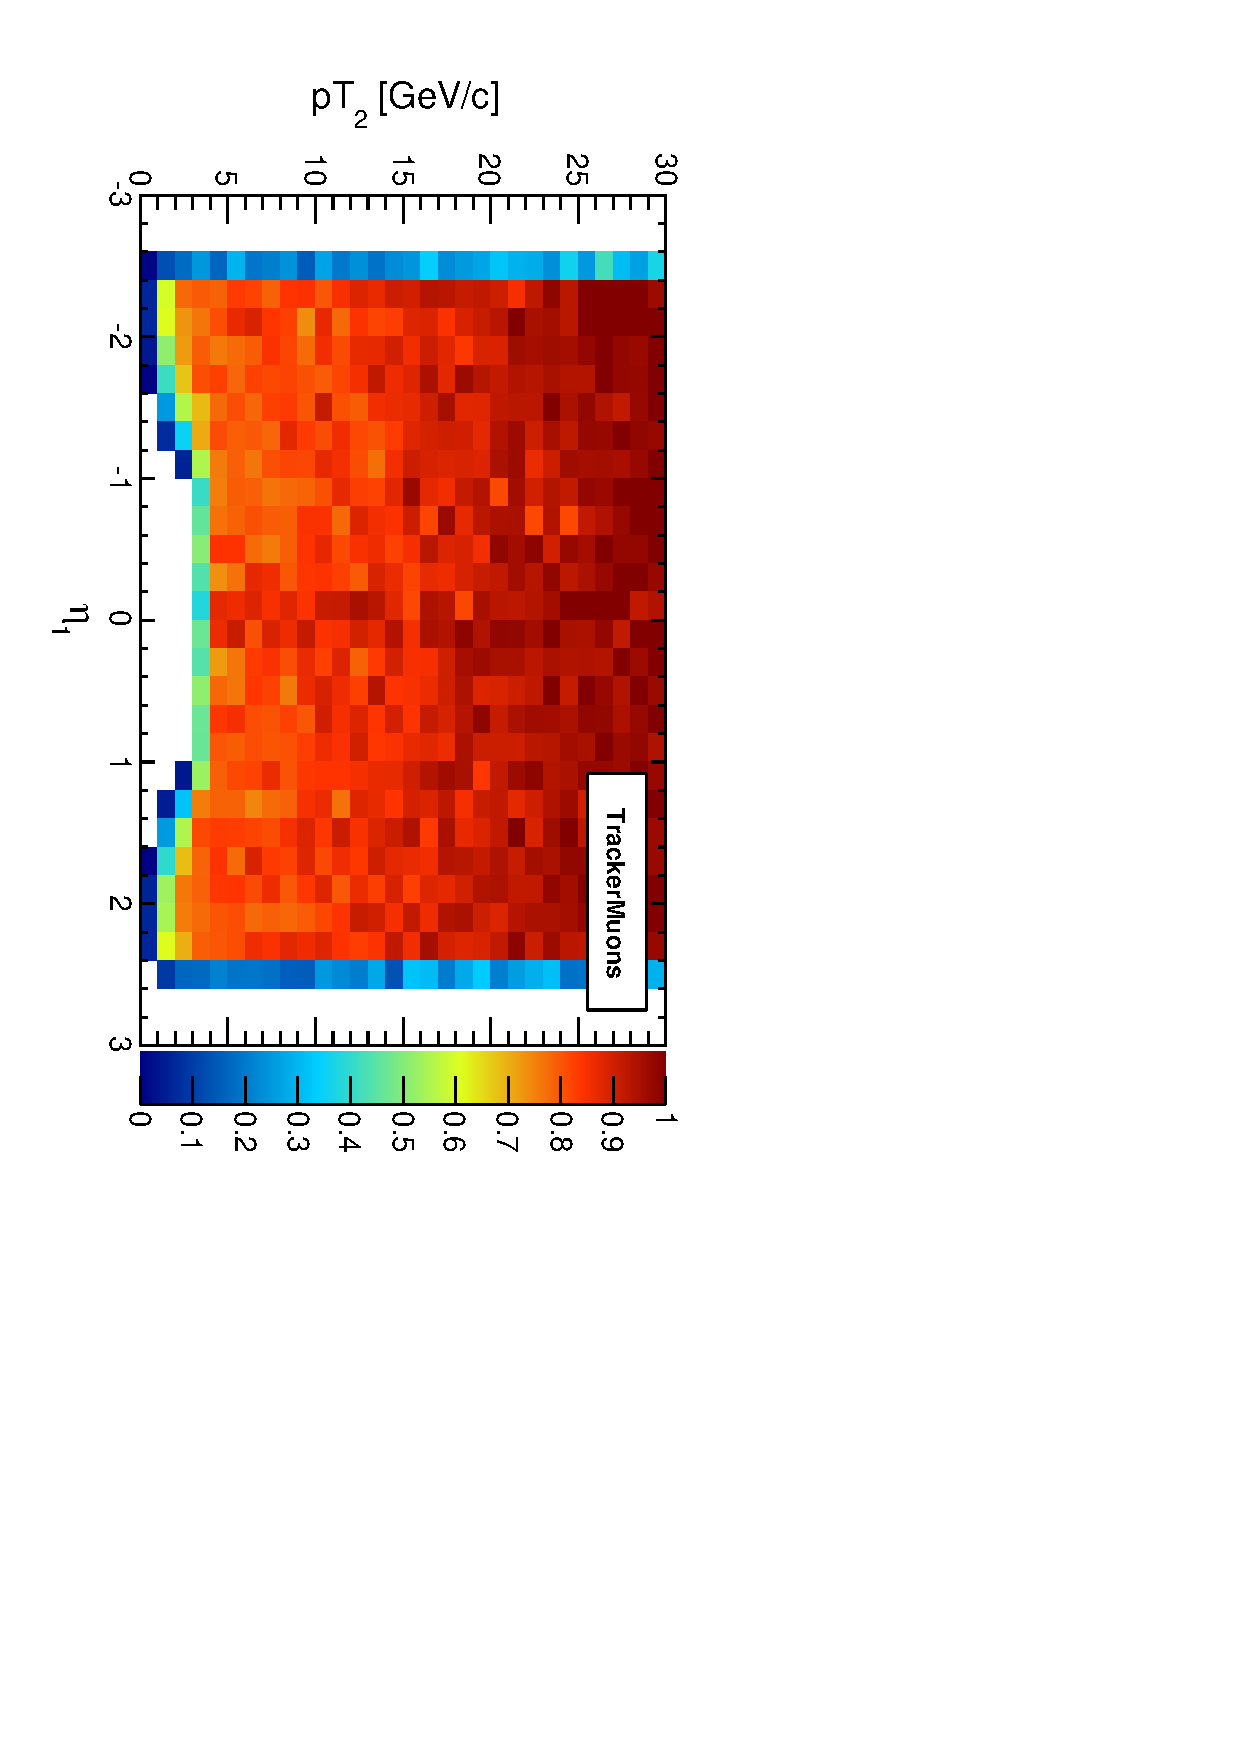
\includegraphics[height=\linewidth, angle=90]{pt2vseta1_TrackerMuons.pdf}}
\only<2>{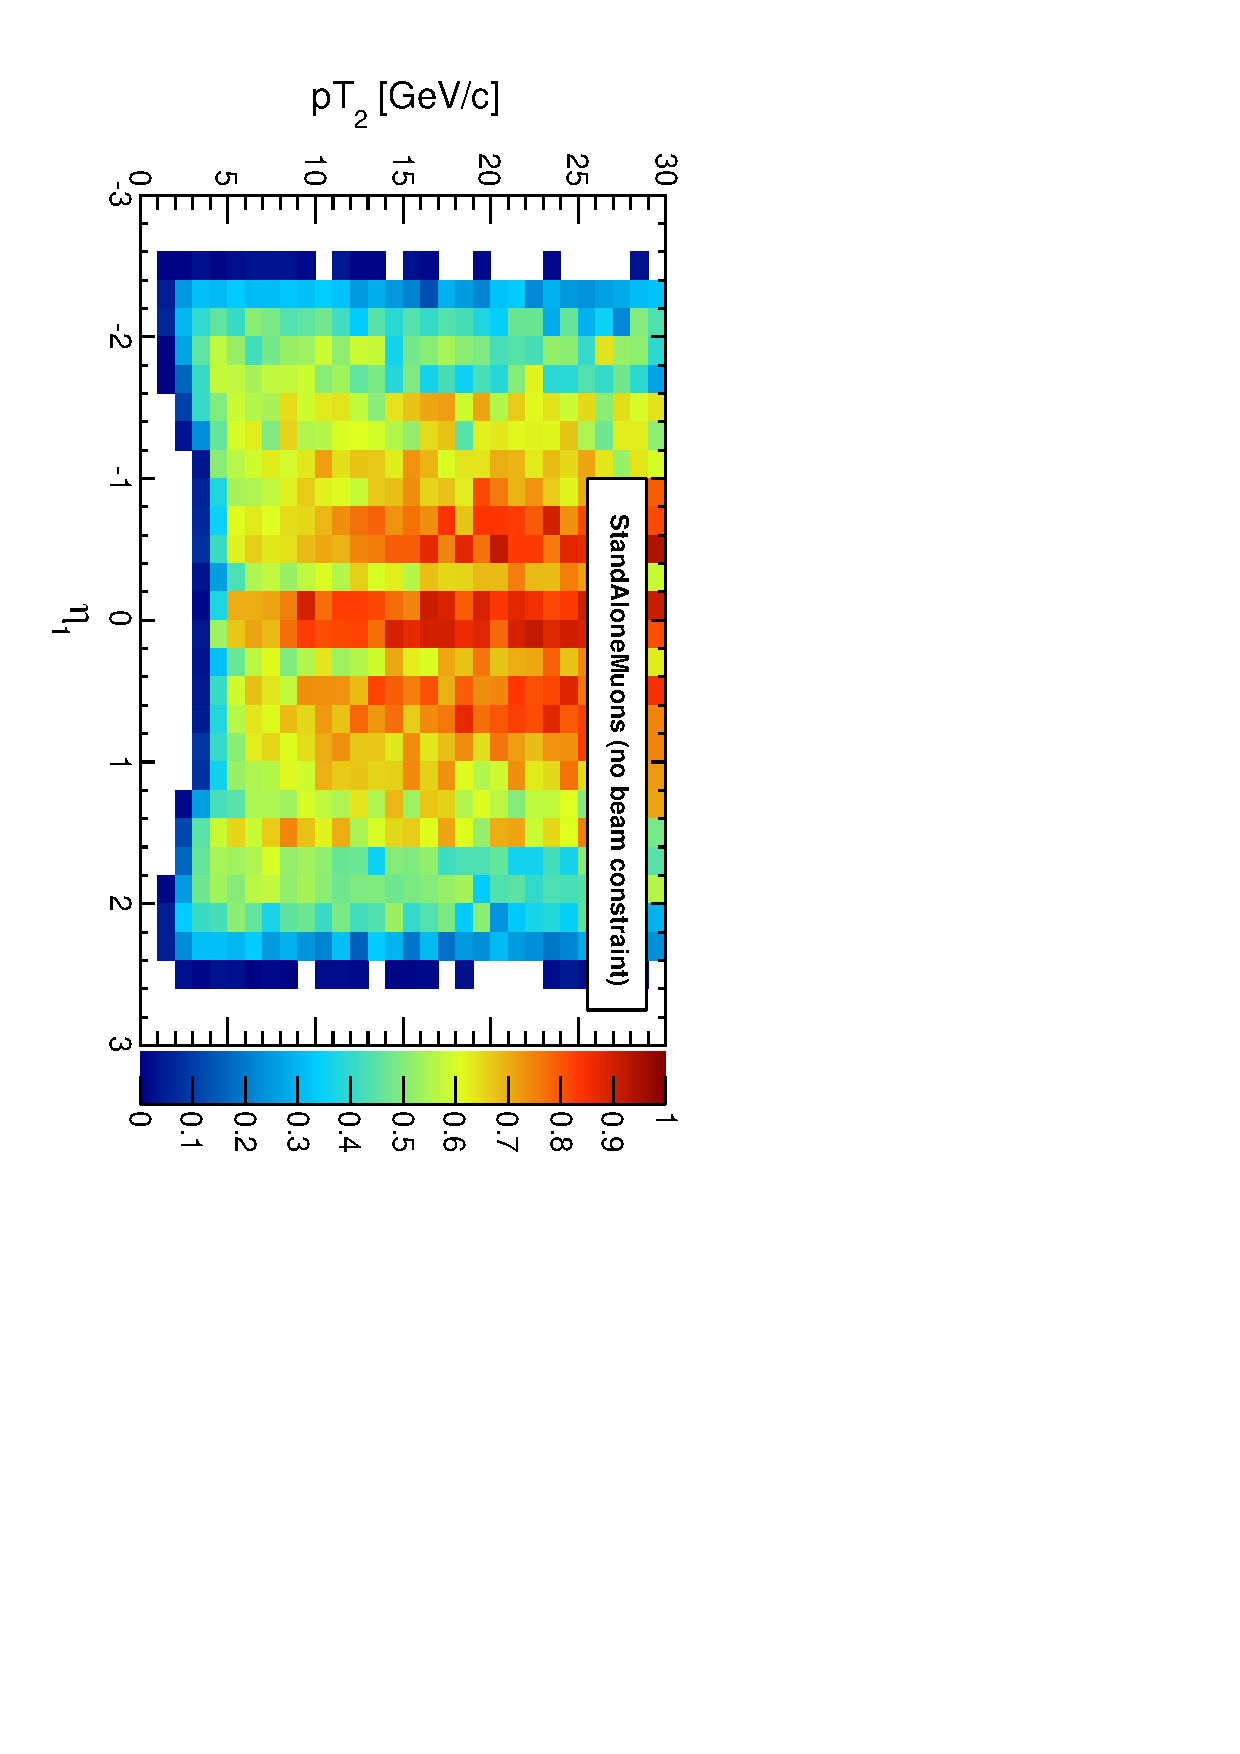
\includegraphics[height=\linewidth, angle=90]{pt2vseta1_StandAloneDefault.pdf}}
\only<3>{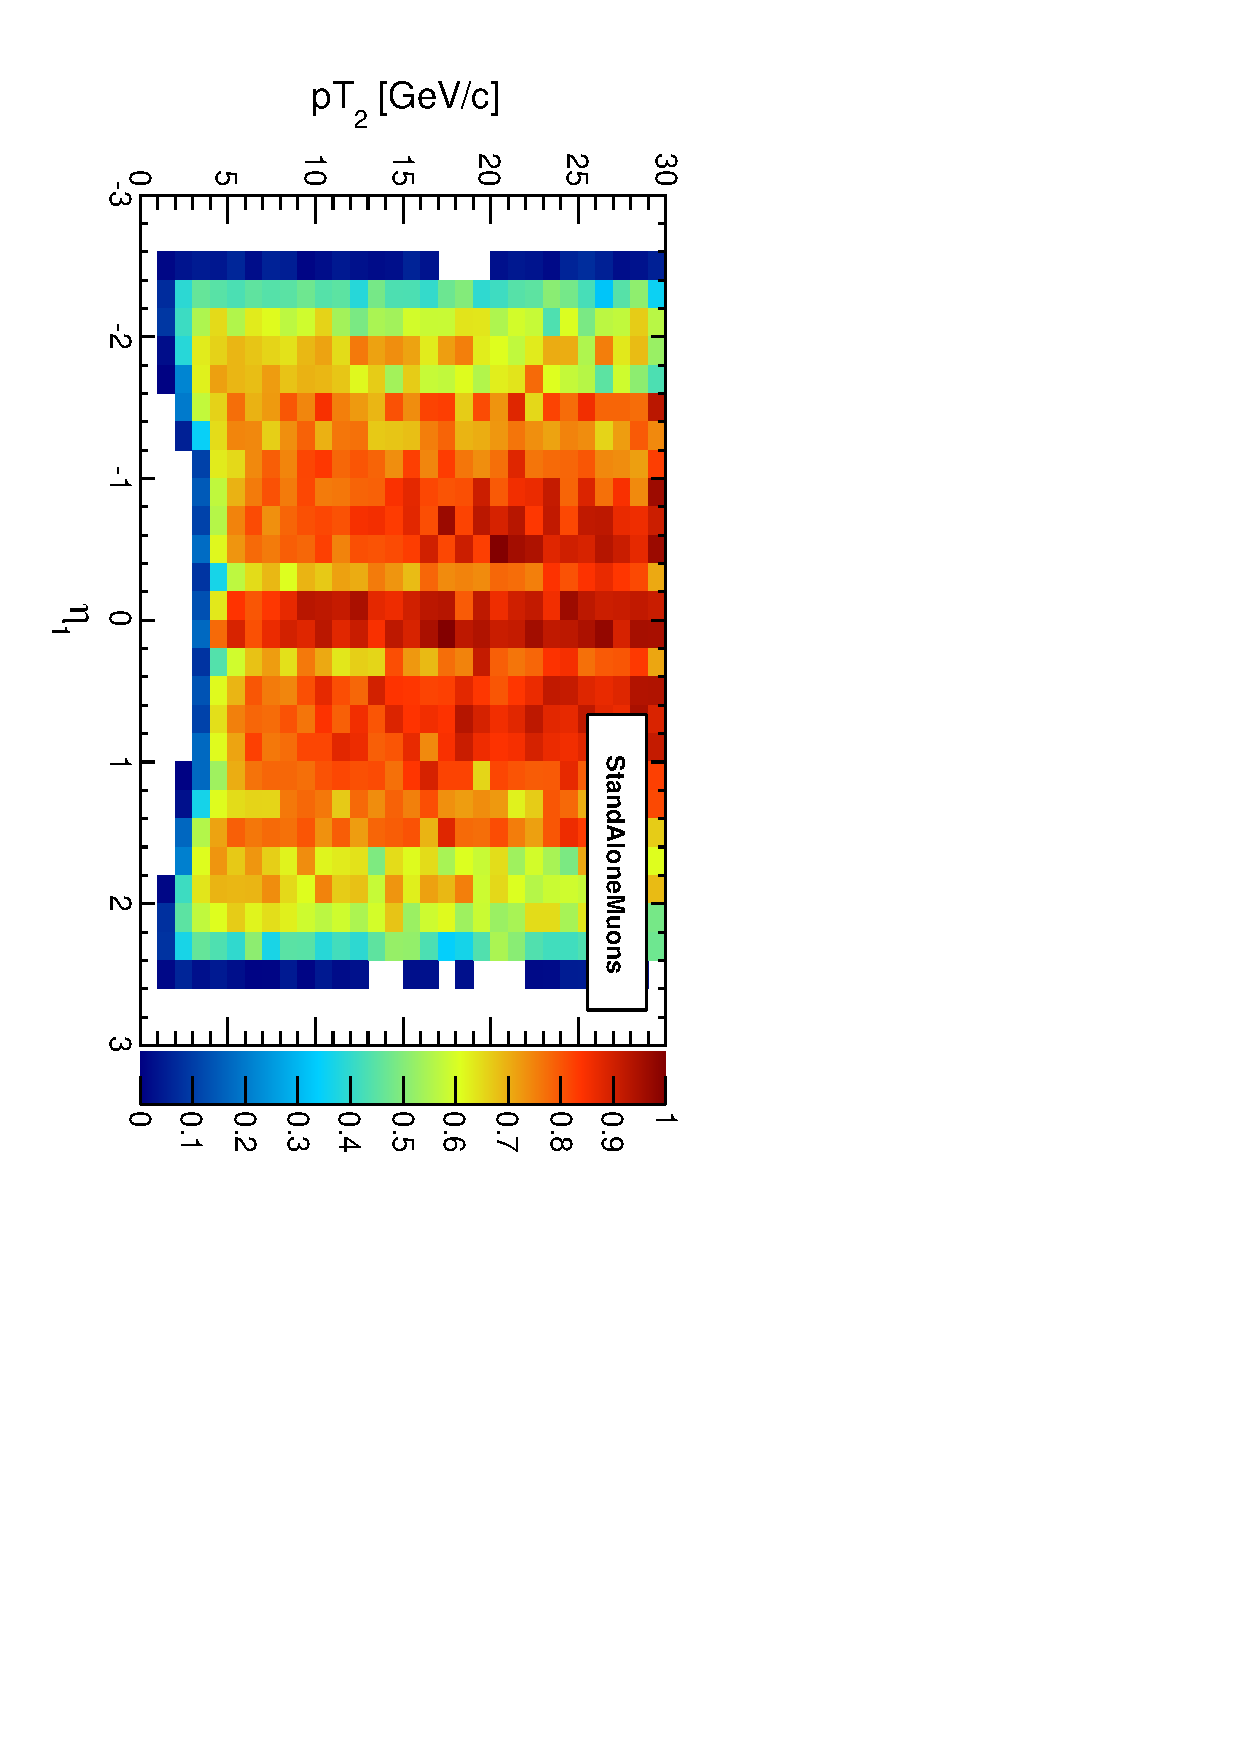
\includegraphics[height=\linewidth, angle=90]{pt2vseta1_StandAloneUpdatedDefault.pdf}}
\only<4>{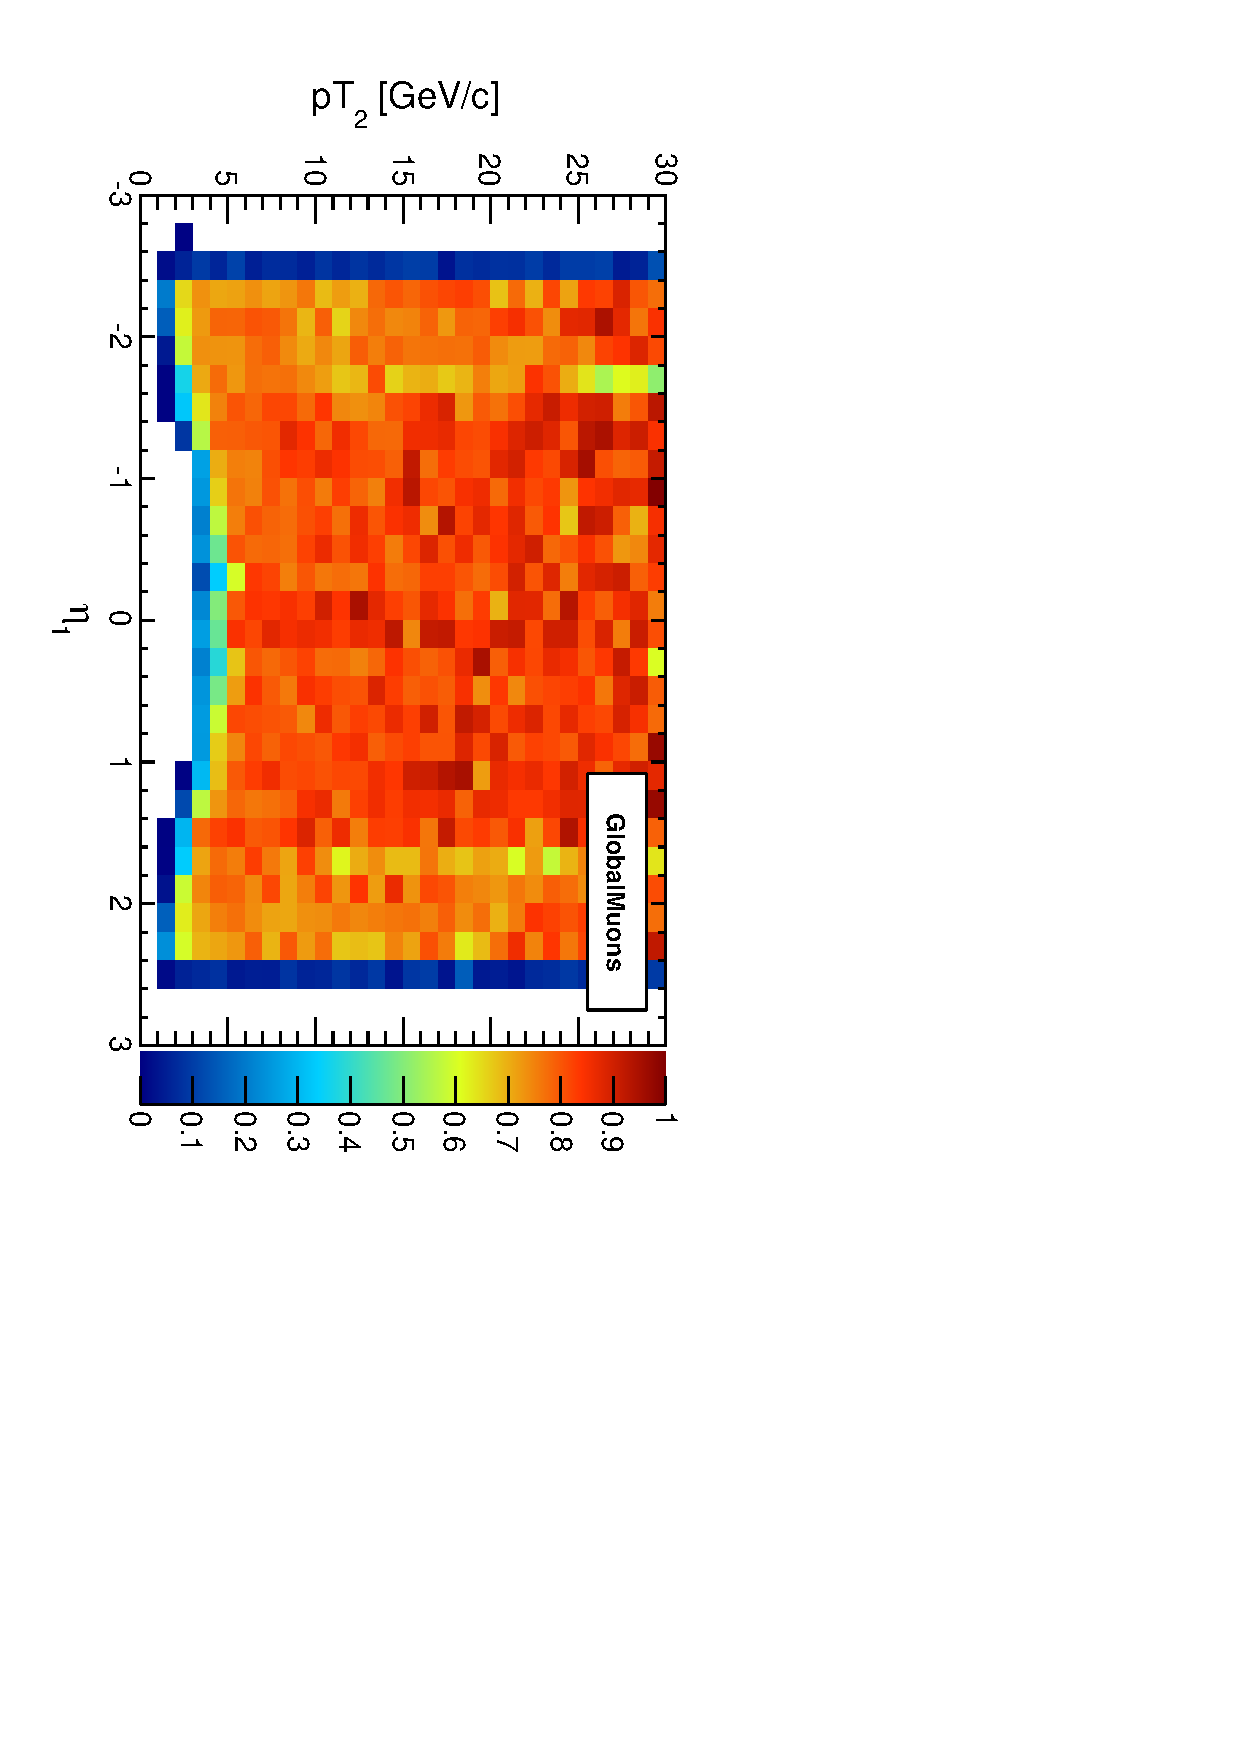
\includegraphics[height=\linewidth, angle=90]{pt2vseta1_GlobalMuons.pdf}}

\only<1>{\vspace{-0.5 cm} From a dimuon gun uniform in dimuon mass, $p_T$ (up to 100~GeV/$c$), and $\eta$, decaying spherically (used for all efficiency studies)}
\only<2>{\vspace{-0.5 cm} Also tested the StandAlone-SET algorithm, but that has a very low efficiency for nearby pairs (apparently has a cut against muons being within 10~cm in $z$ in muon chambers)}
\only<3>{StandAloneMuons with a beamline constraint has somewhat higher efficiency}
\only<4>{But not enough to explain the GlobalMuon efficiency: how can GlobalMuon efficiency be higher than StandAlone???}
\end{frame}

\begin{frame}
\frametitle{Efficiency for physics}

Assuming $pT_2 > 5$~GeV/$c$ and $|\eta_1| < 2.4$ are satisfied (that's the denominator), how sensitive are we to muon jets across the mass/momentum range?

\vfill
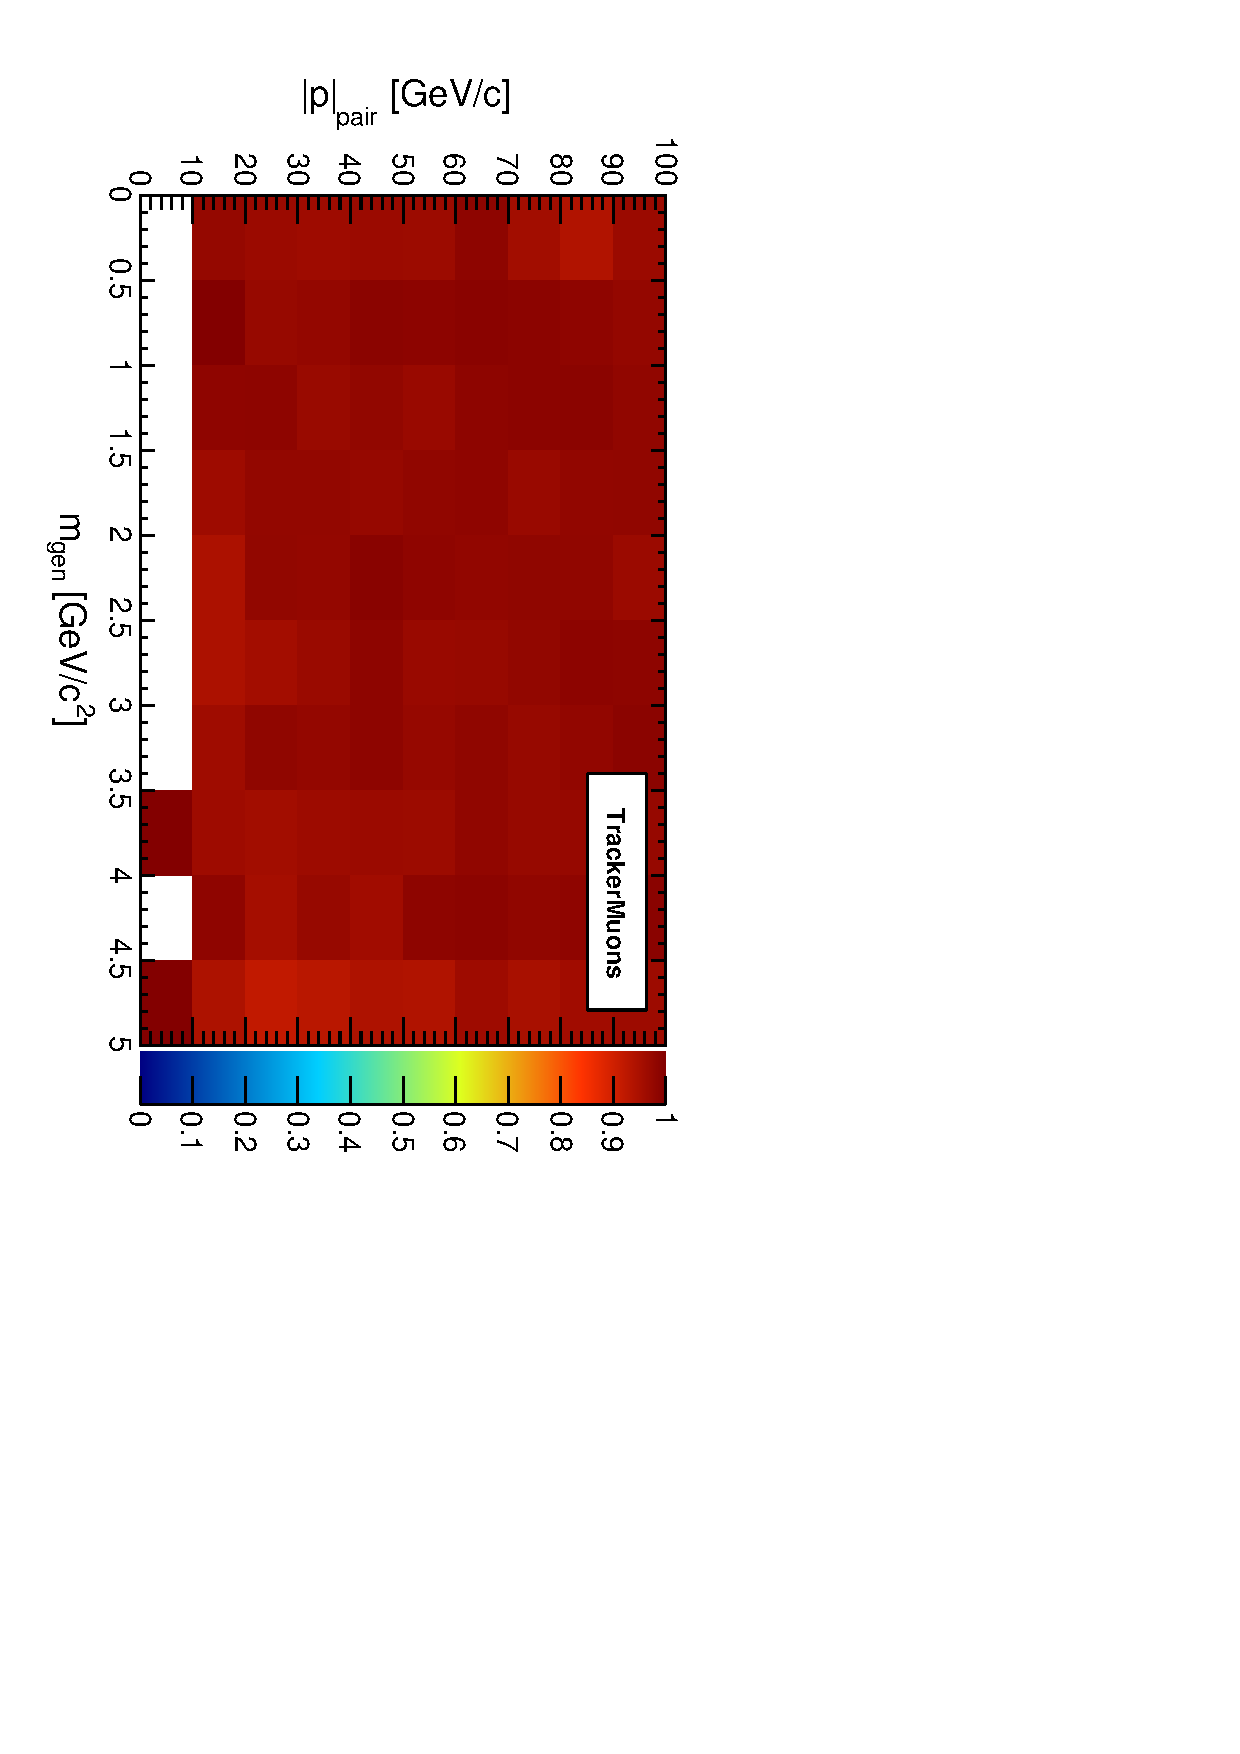
\includegraphics[height=0.5\linewidth, angle=90]{pairpmagvsmass_TrackerMuons.pdf}
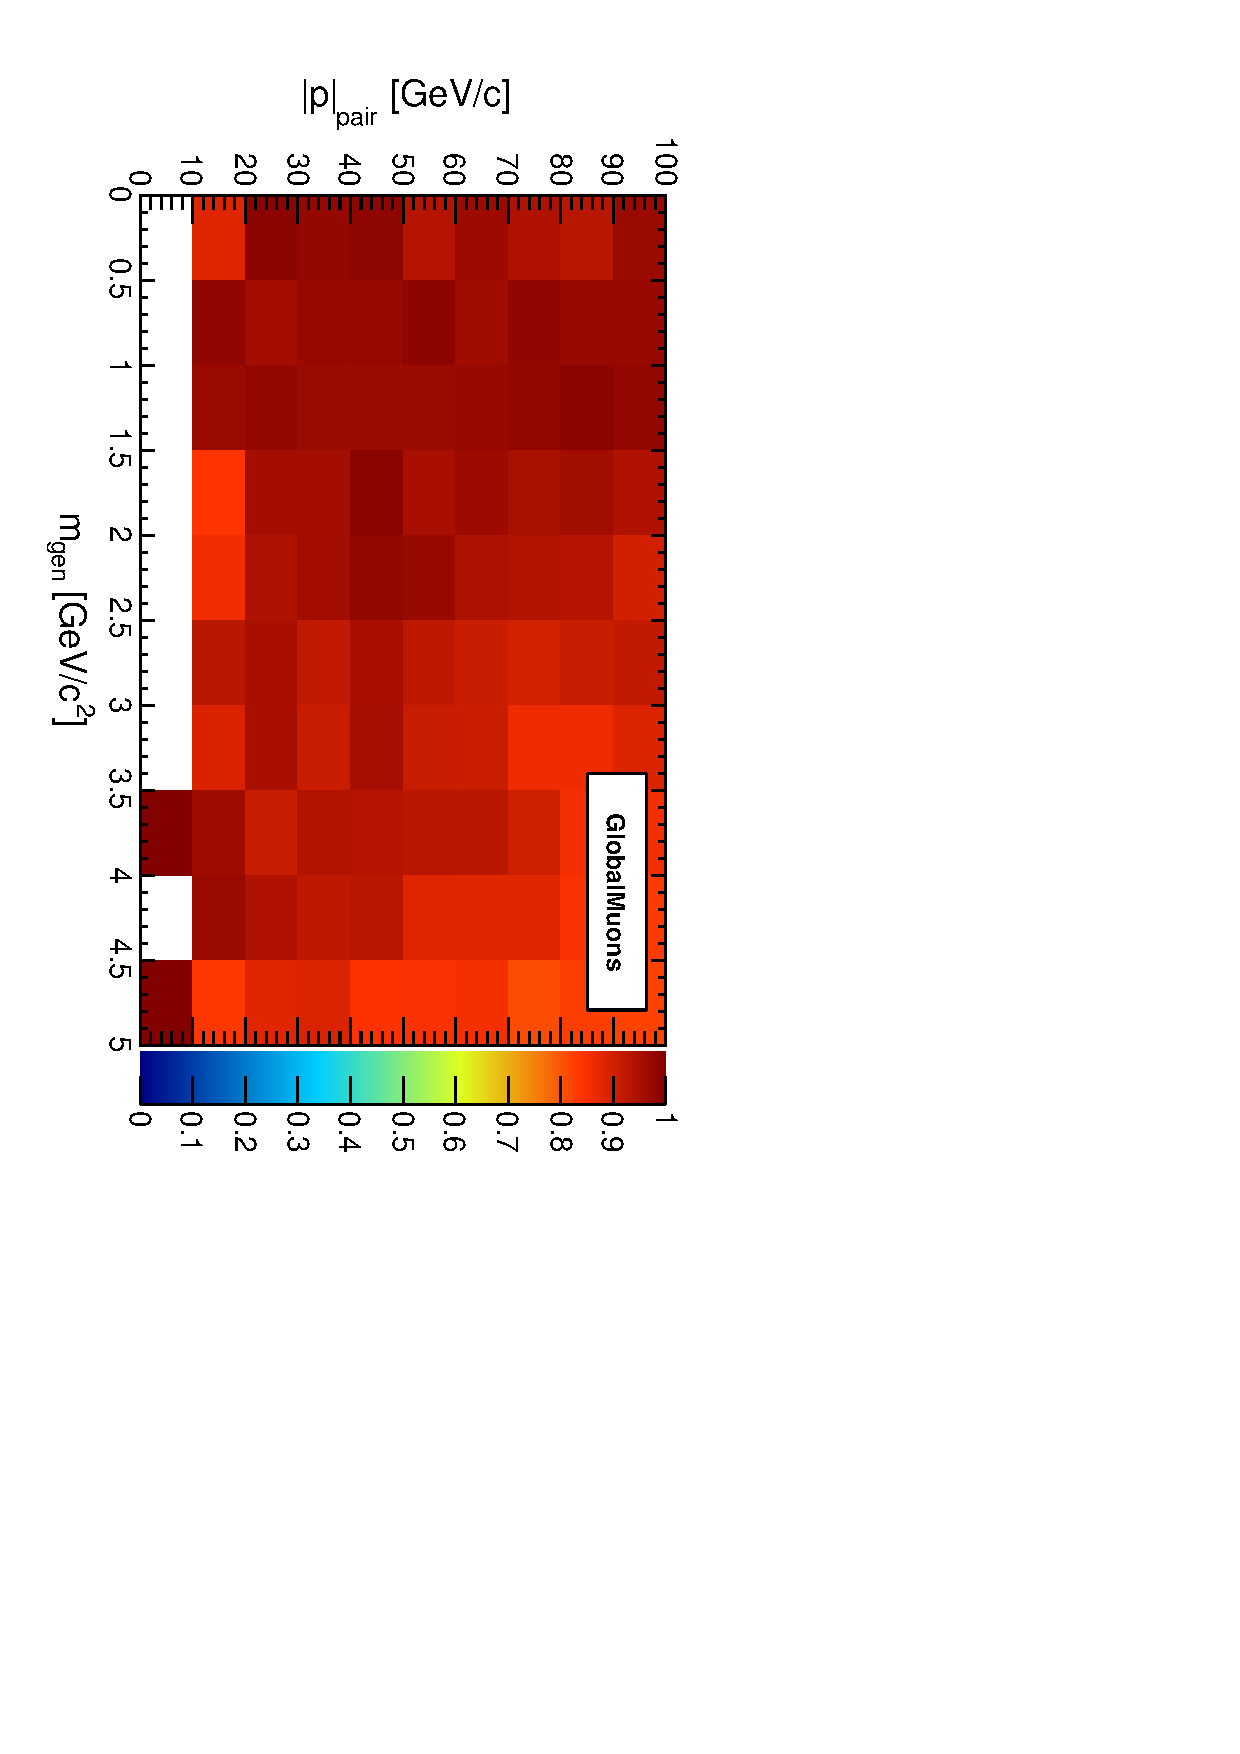
\includegraphics[height=0.5\linewidth, angle=90]{pairpmagvsmass_GlobalMuons.pdf}

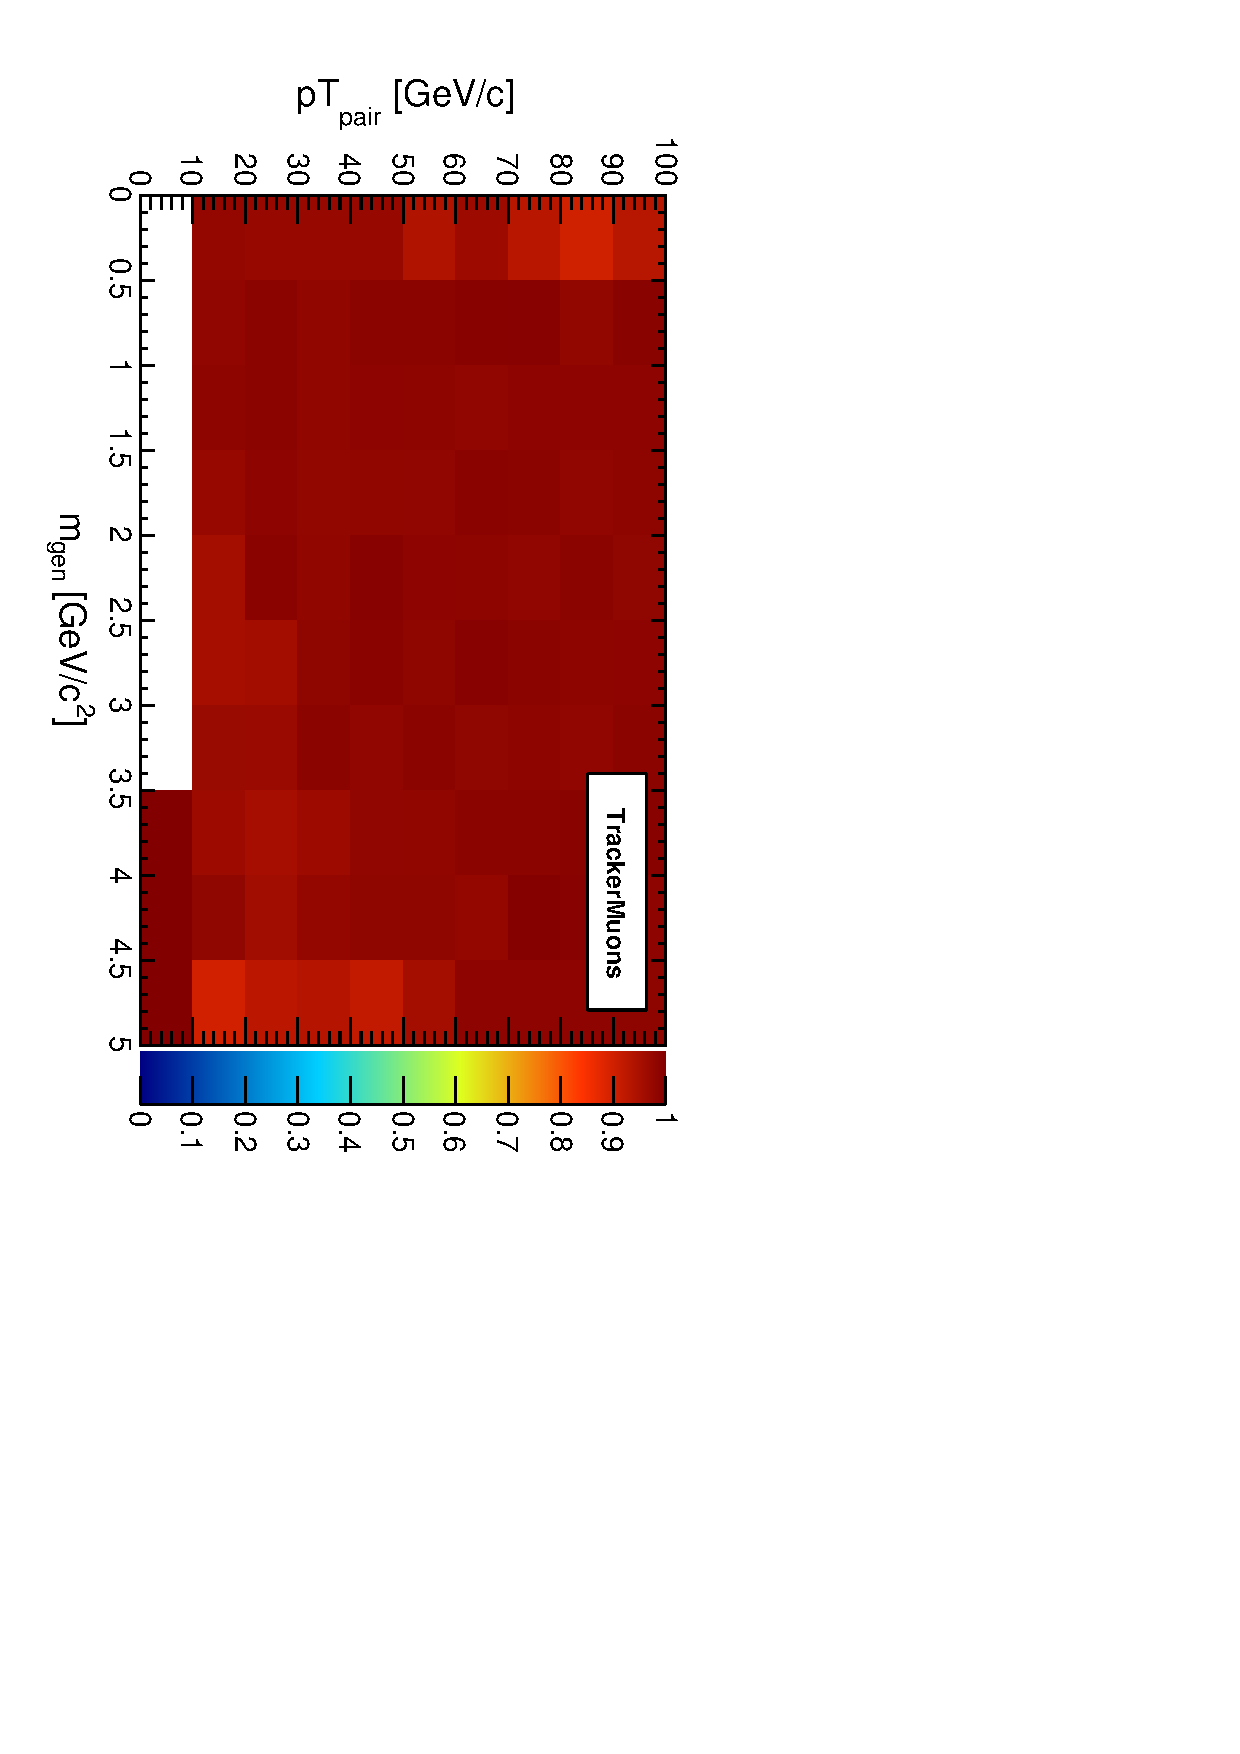
\includegraphics[height=0.5\linewidth, angle=90]{pairptvsmass_TrackerMuons.pdf}
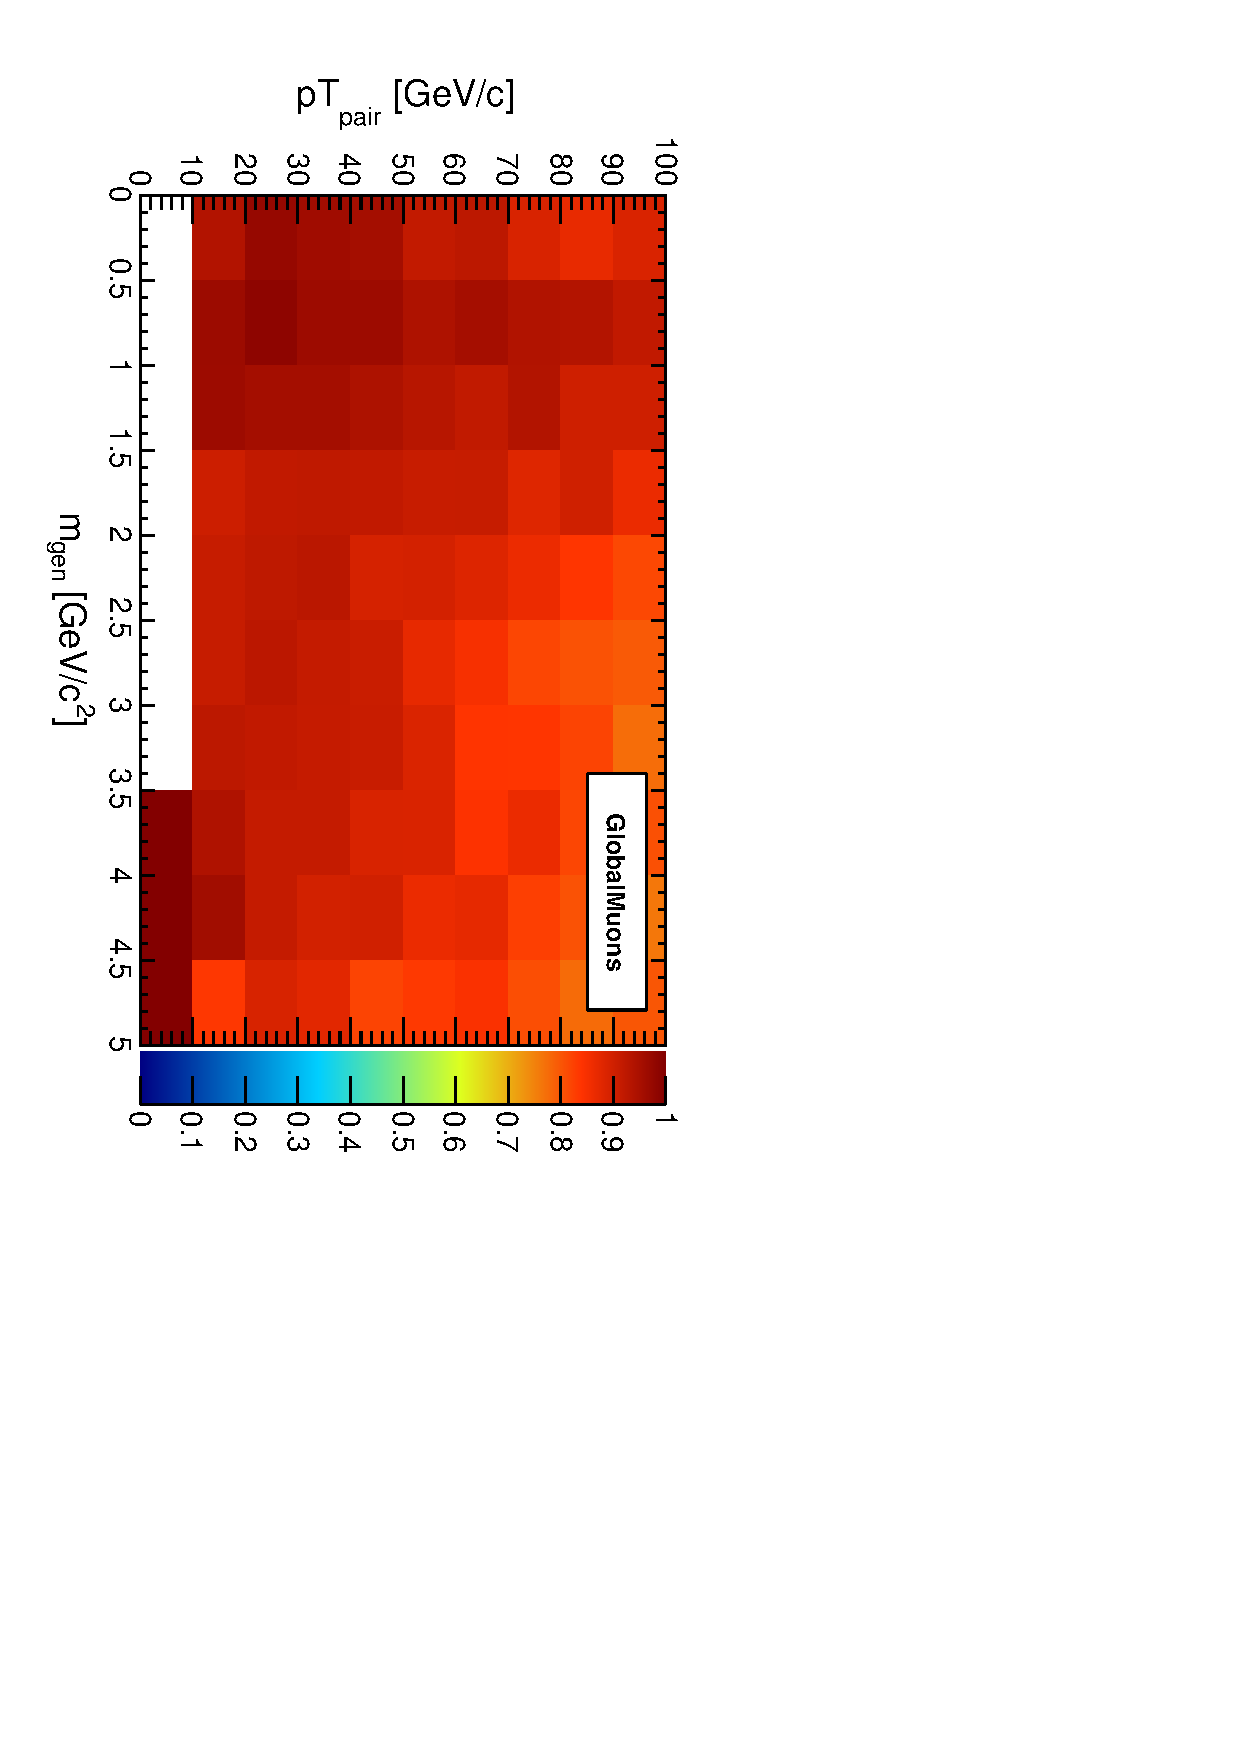
\includegraphics[height=0.5\linewidth, angle=90]{pairptvsmass_GlobalMuons.pdf}
\end{frame}

\begin{frame}
\frametitle{Separation in muon barrel}
These plots also assume $pT_2 > 5$~GeV/$c$ and $|\eta_1| < 2.4$ and ask what is the probability of reconstructing both muons as a function of where they cross in the muon system ($\Delta \phi = \phi_{\mu^+} - \phi_{\mu^-}$, $\Delta z = z_{\mu^+} - z_{\mu^-}$).

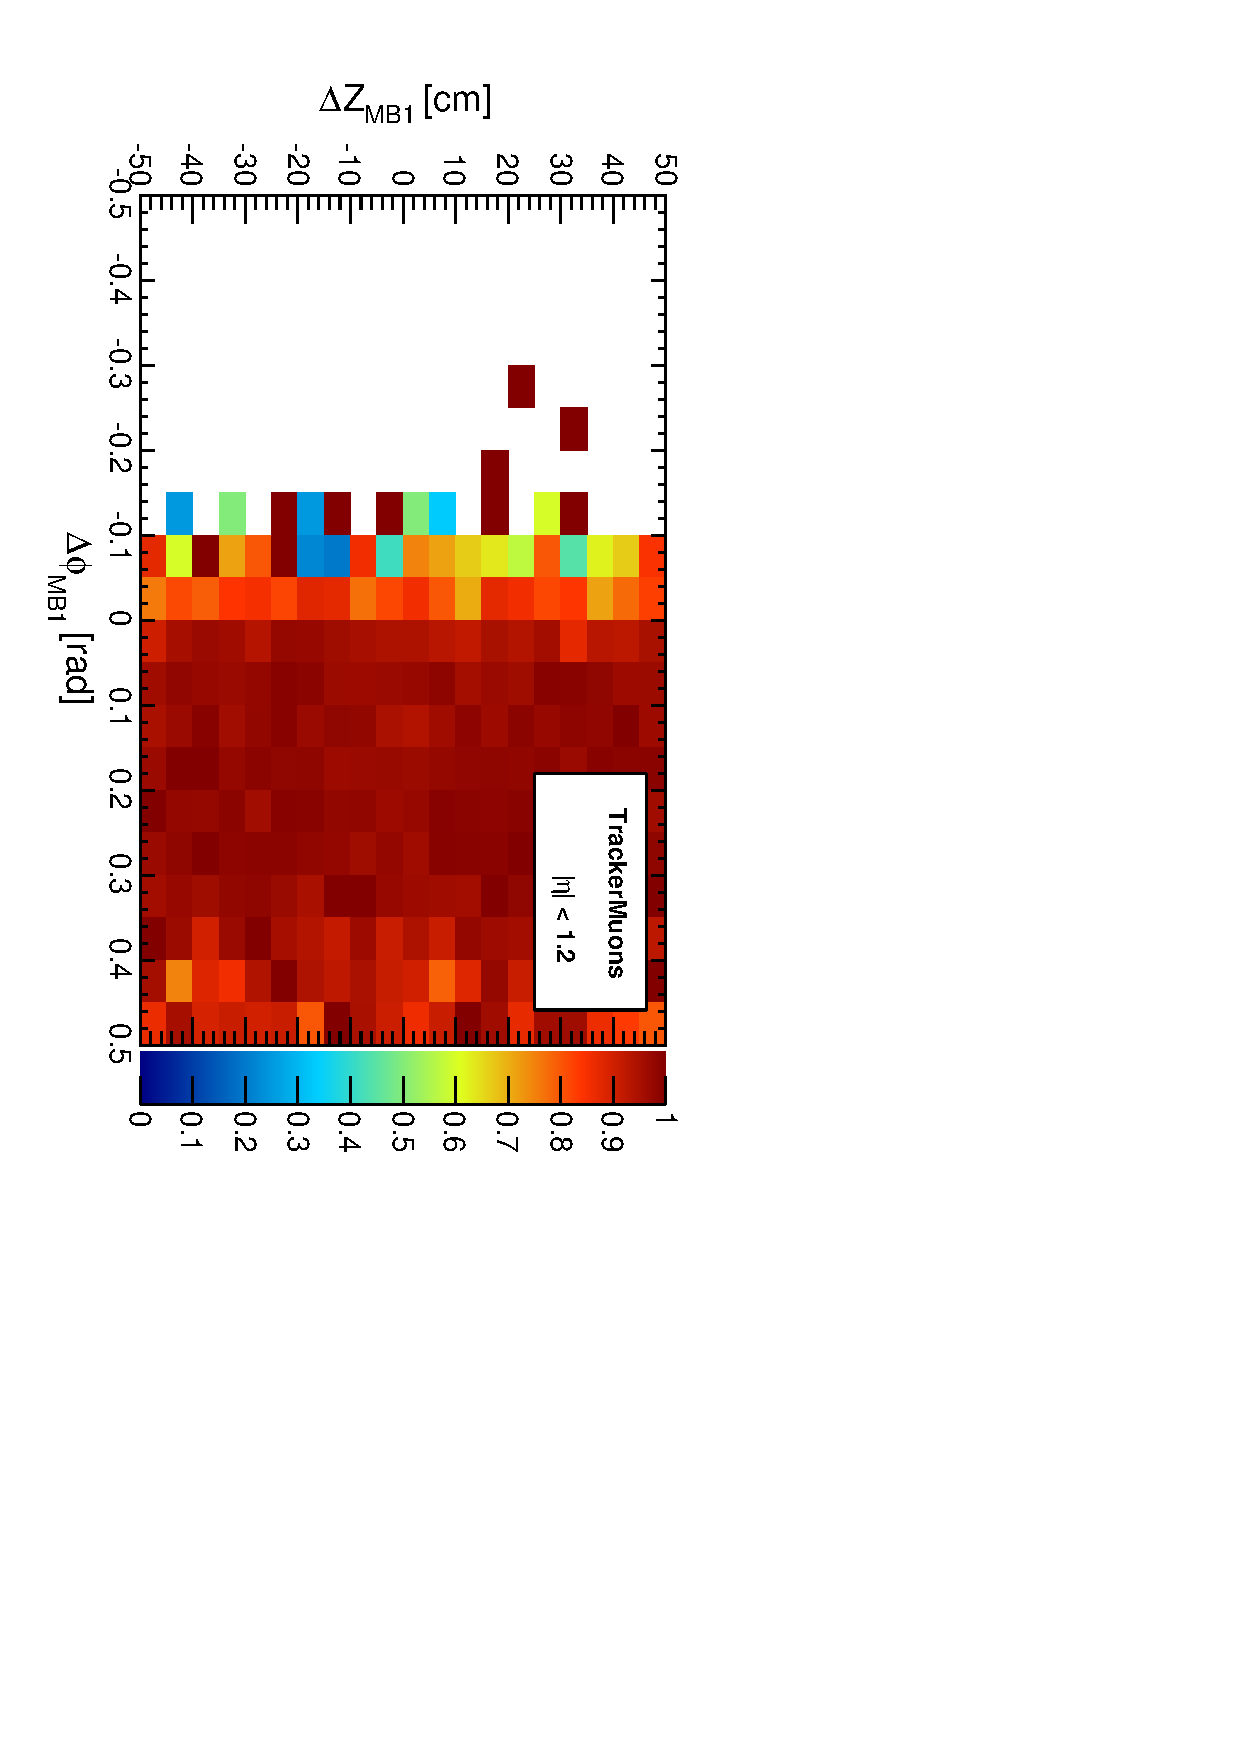
\includegraphics[height=0.5\linewidth, angle=90]{mb1_TrackerMuons.pdf}
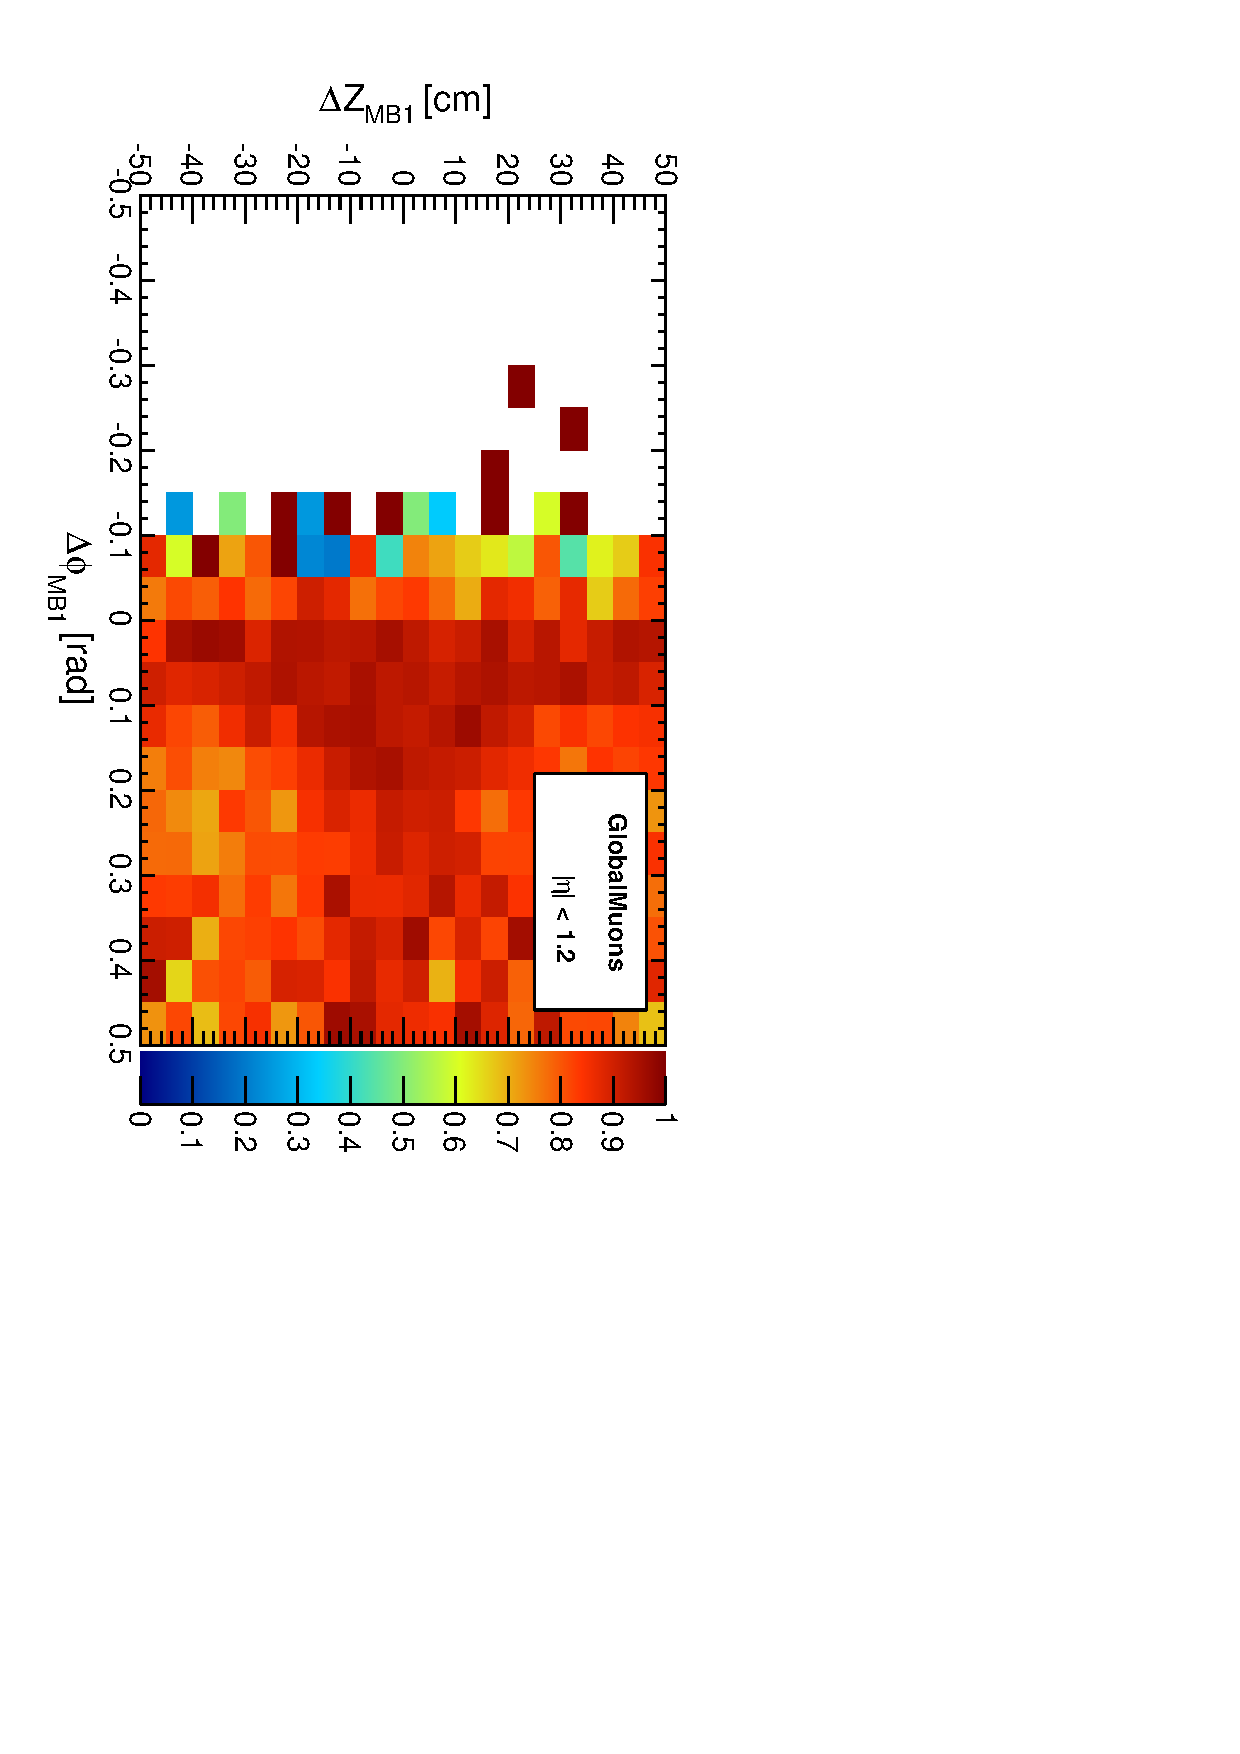
\includegraphics[height=0.5\linewidth, angle=90]{mb1_GlobalMuons.pdf}

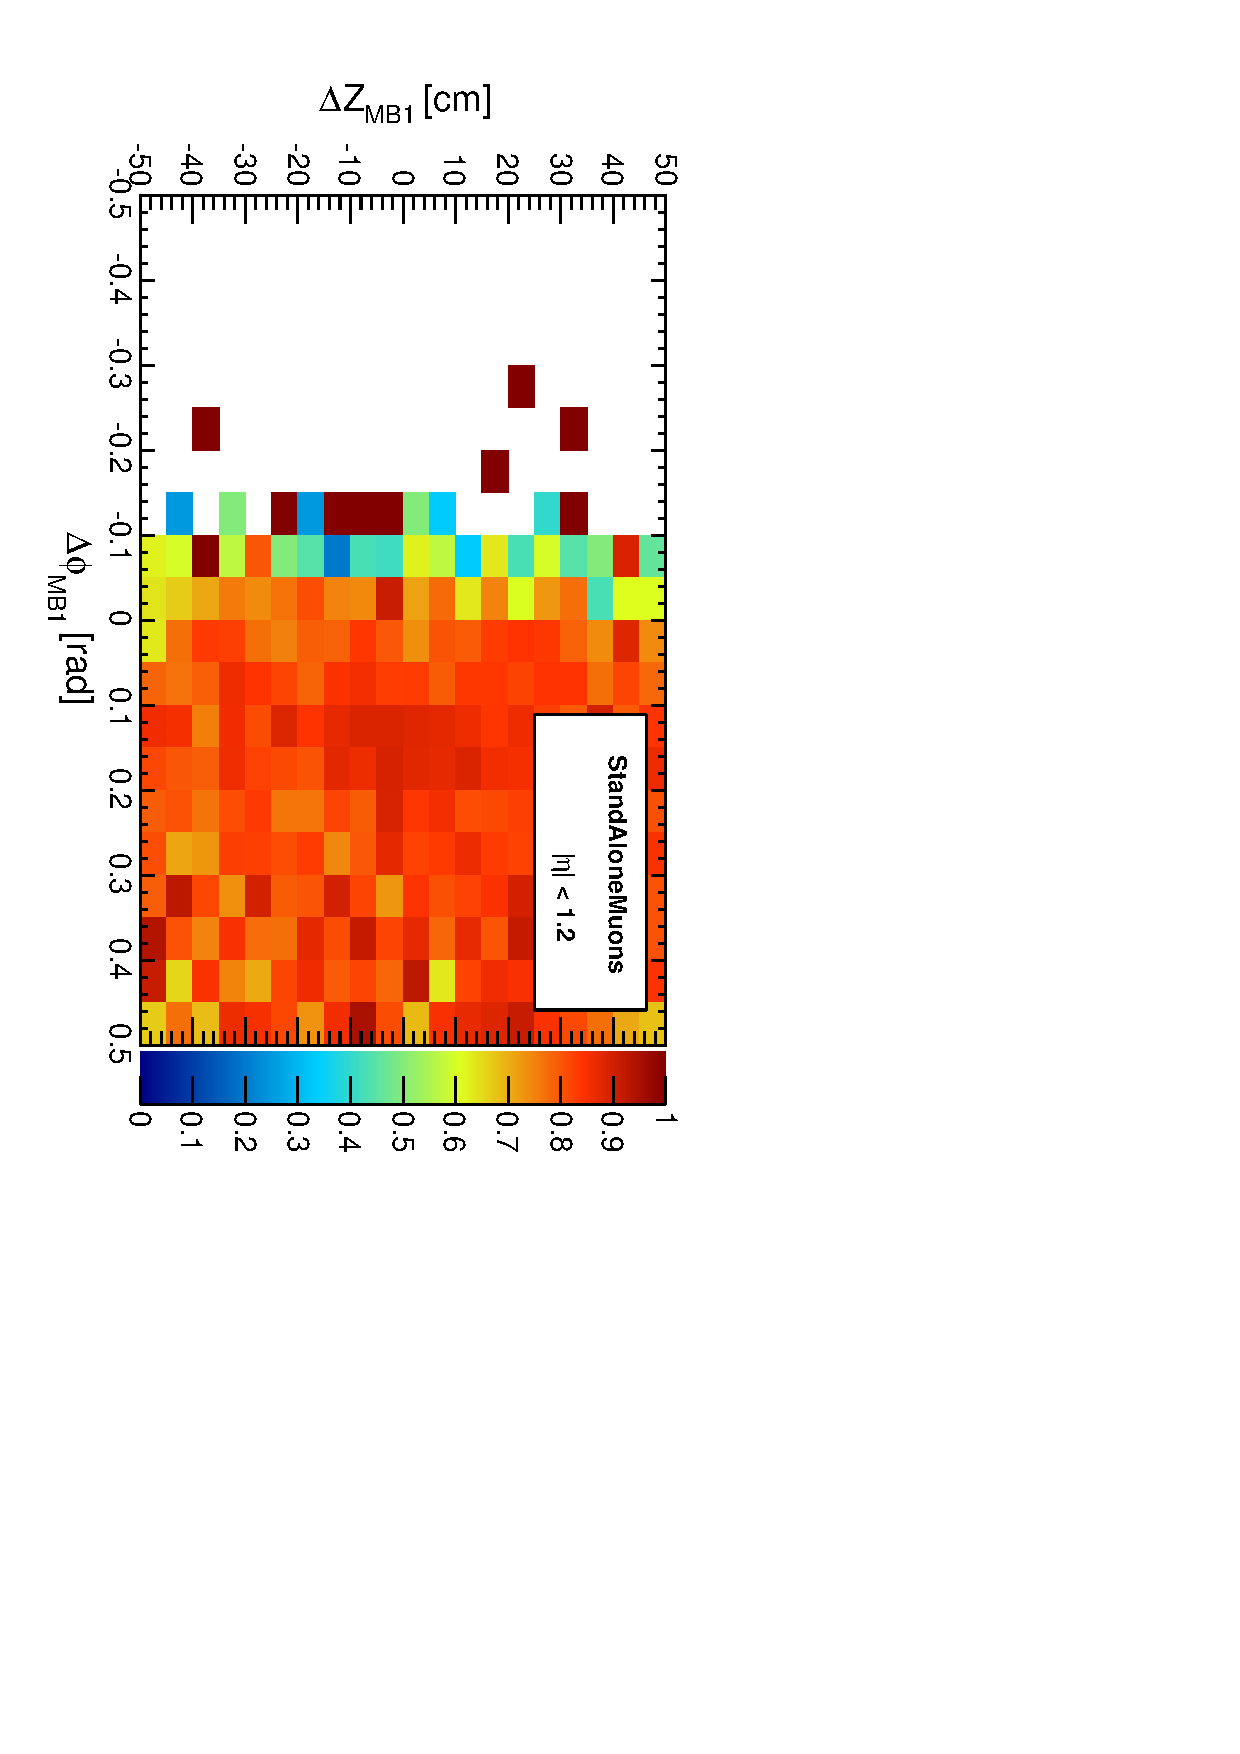
\includegraphics[height=0.5\linewidth, angle=90]{mb1_StandAloneUpdatedDefault.pdf}
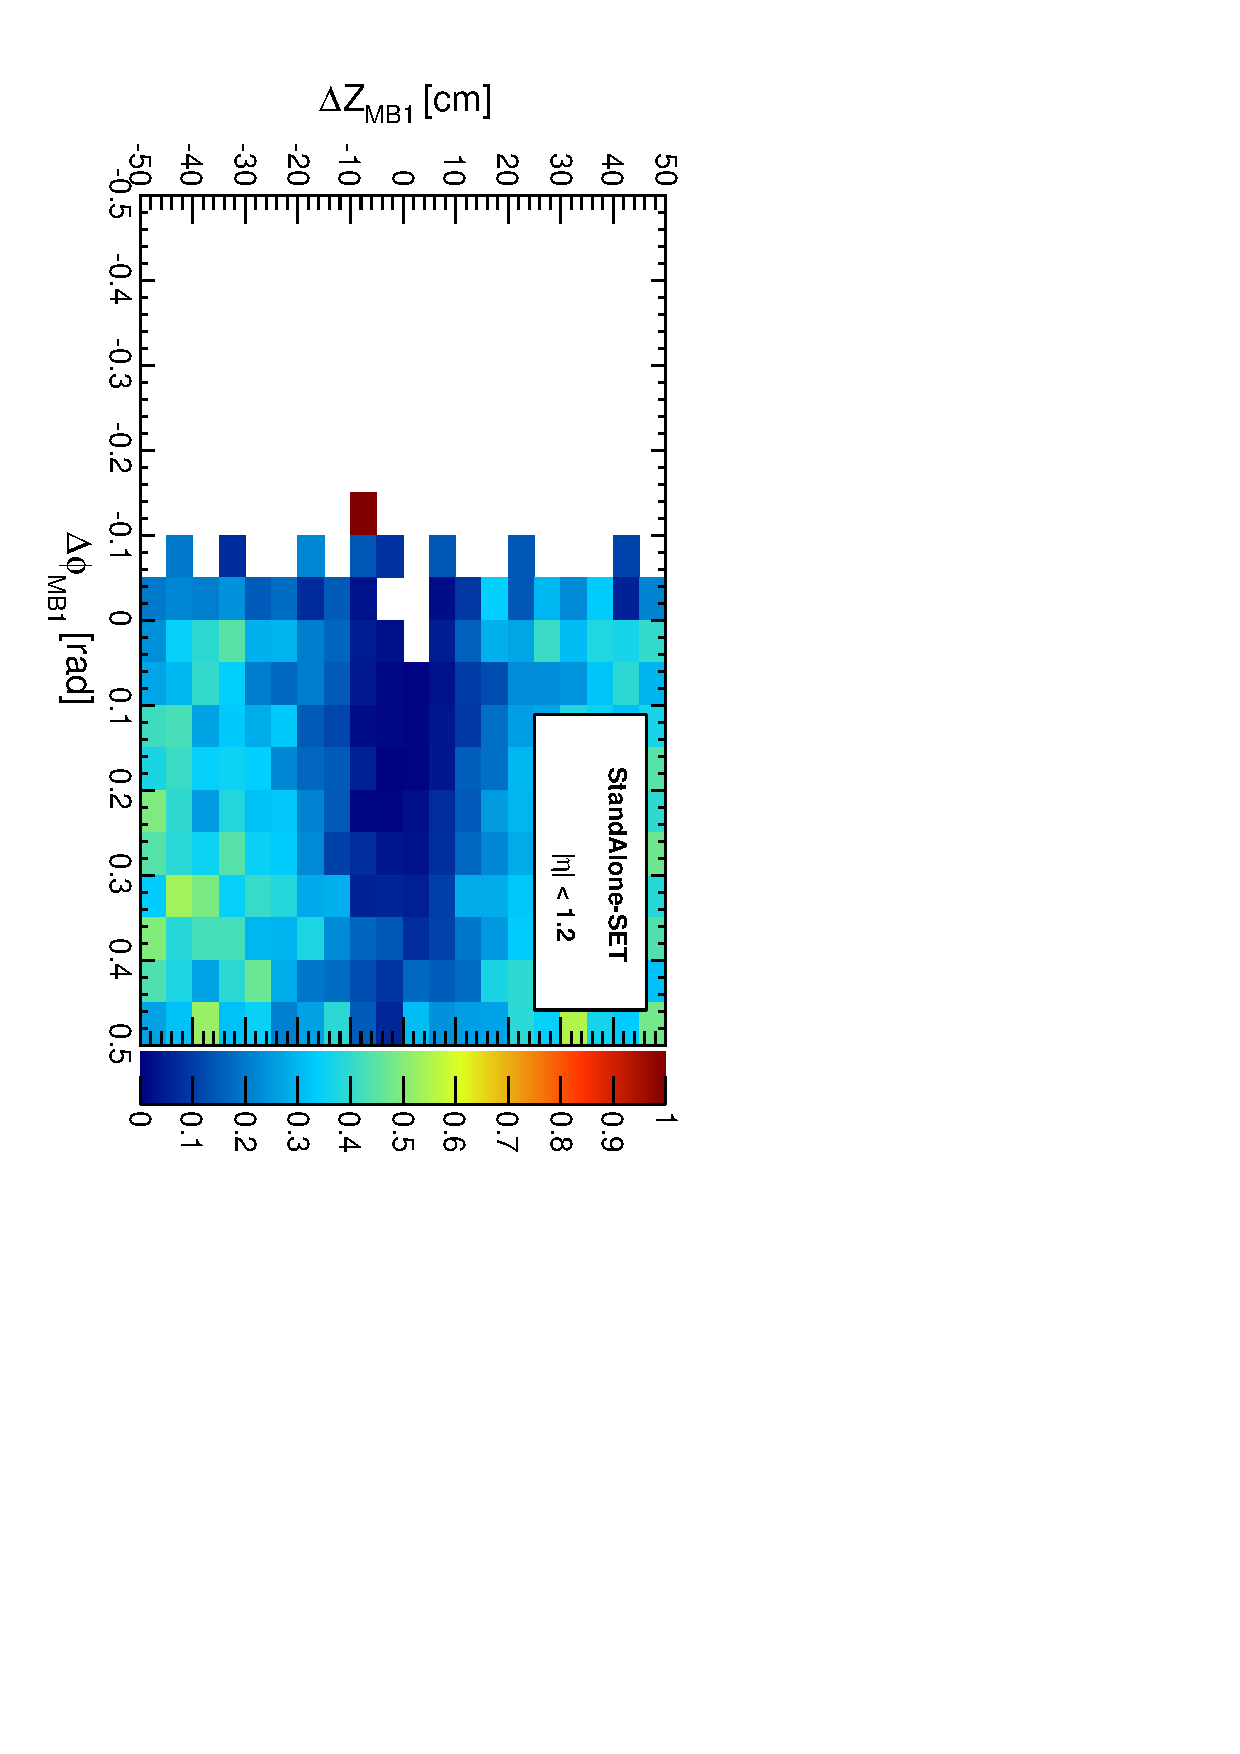
\includegraphics[height=0.5\linewidth, angle=90]{mb1_StandAloneUpdatedSET.pdf}

Stations 2, 3, and 4 are pretty similar.  I'm not sure why the negative sides of these plots are not
illuminated\ldots
\end{frame}

\begin{frame}
\frametitle{Separation in muon endcap}
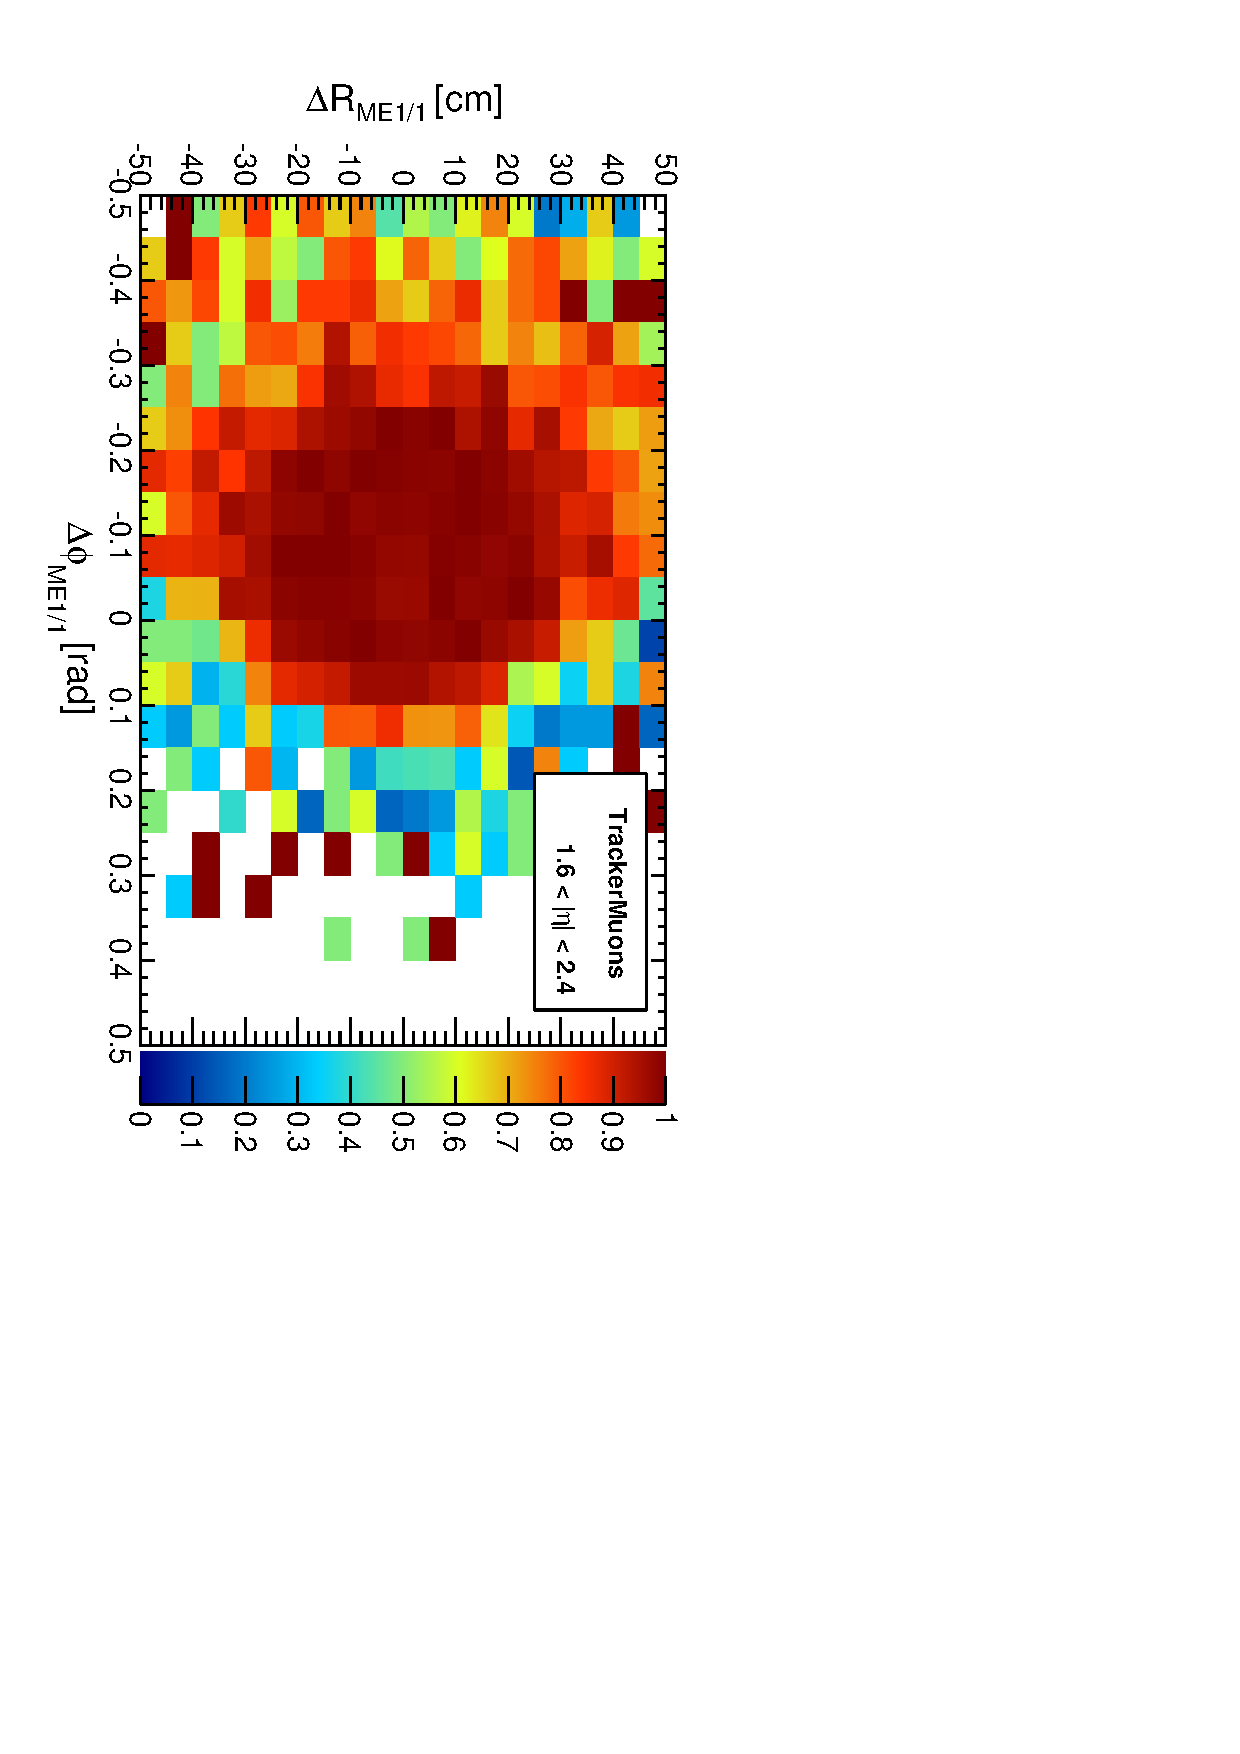
\includegraphics[height=0.5\linewidth, angle=90]{me11_TrackerMuons.pdf}
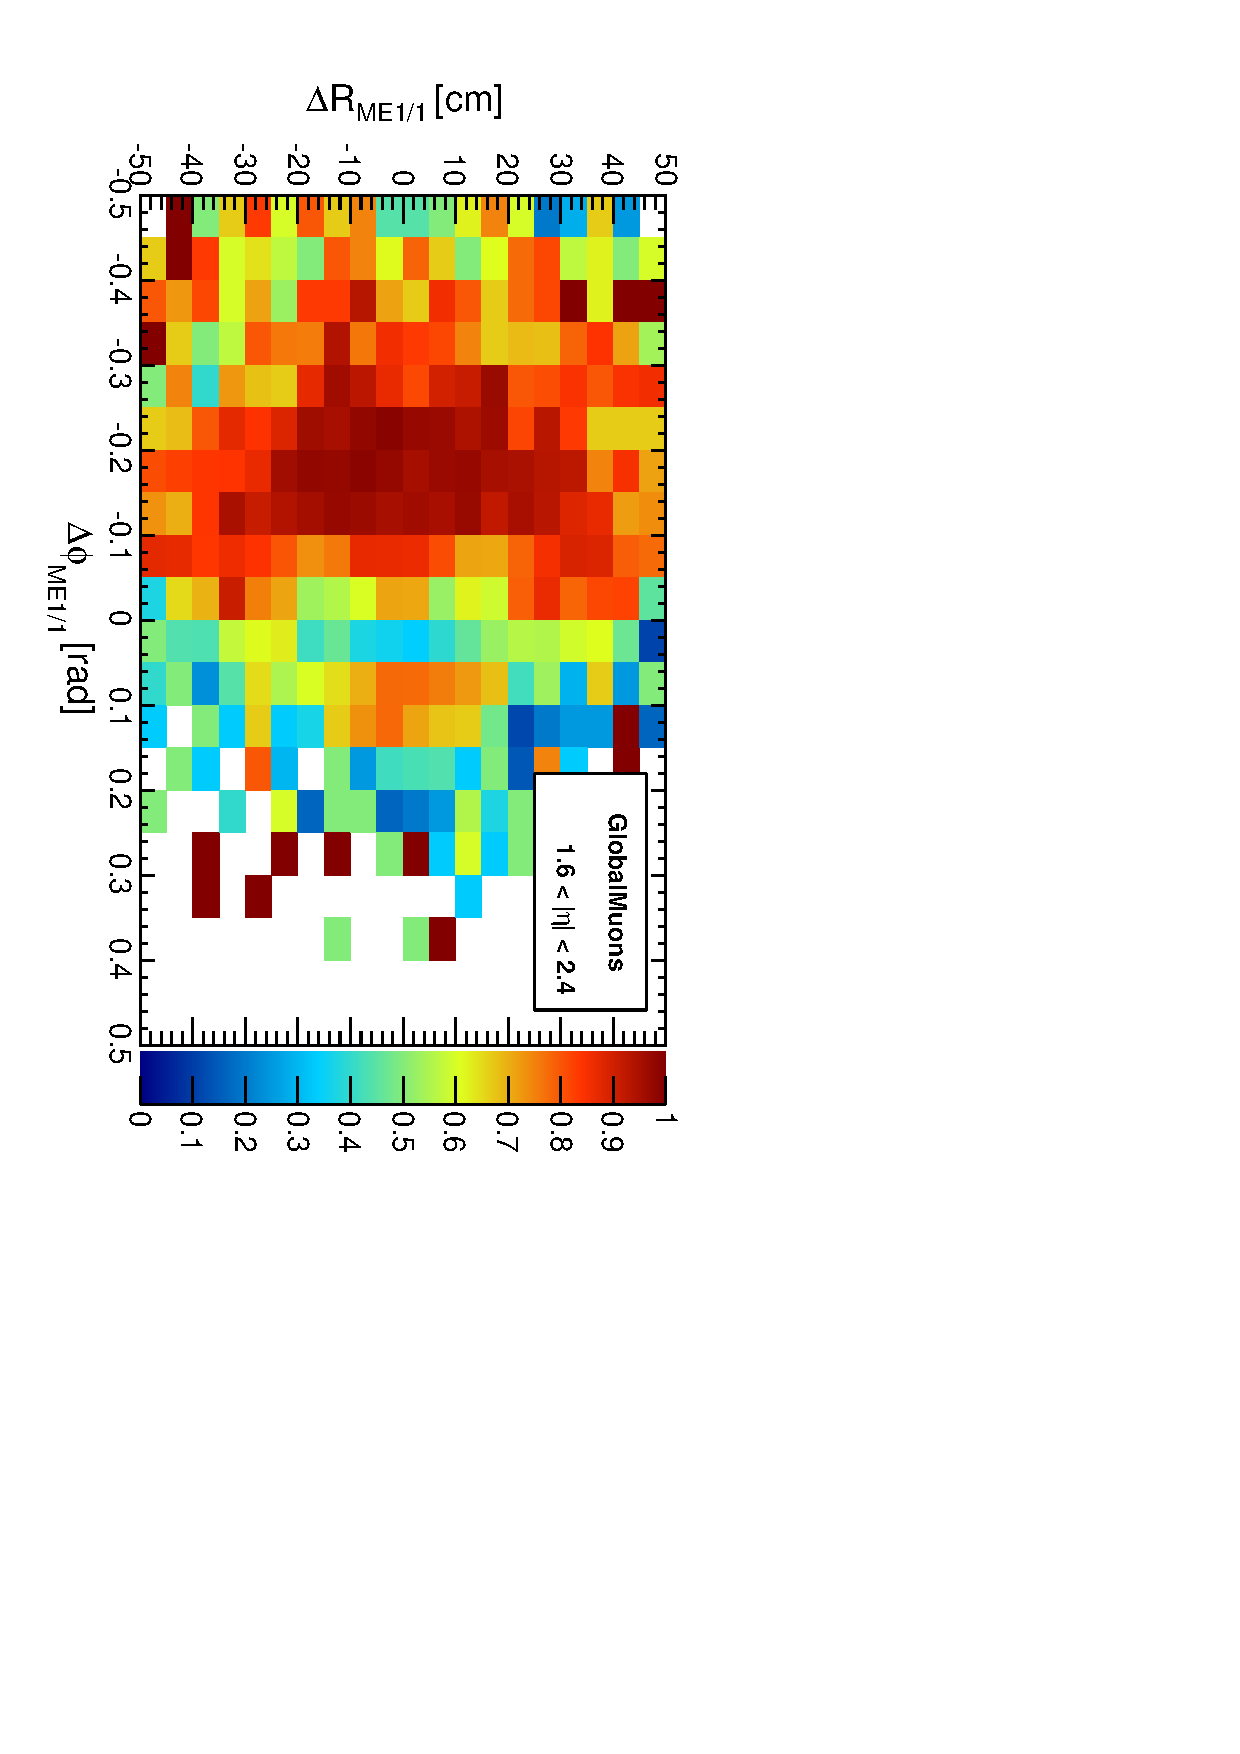
\includegraphics[height=0.5\linewidth, angle=90]{me11_GlobalMuons.pdf}

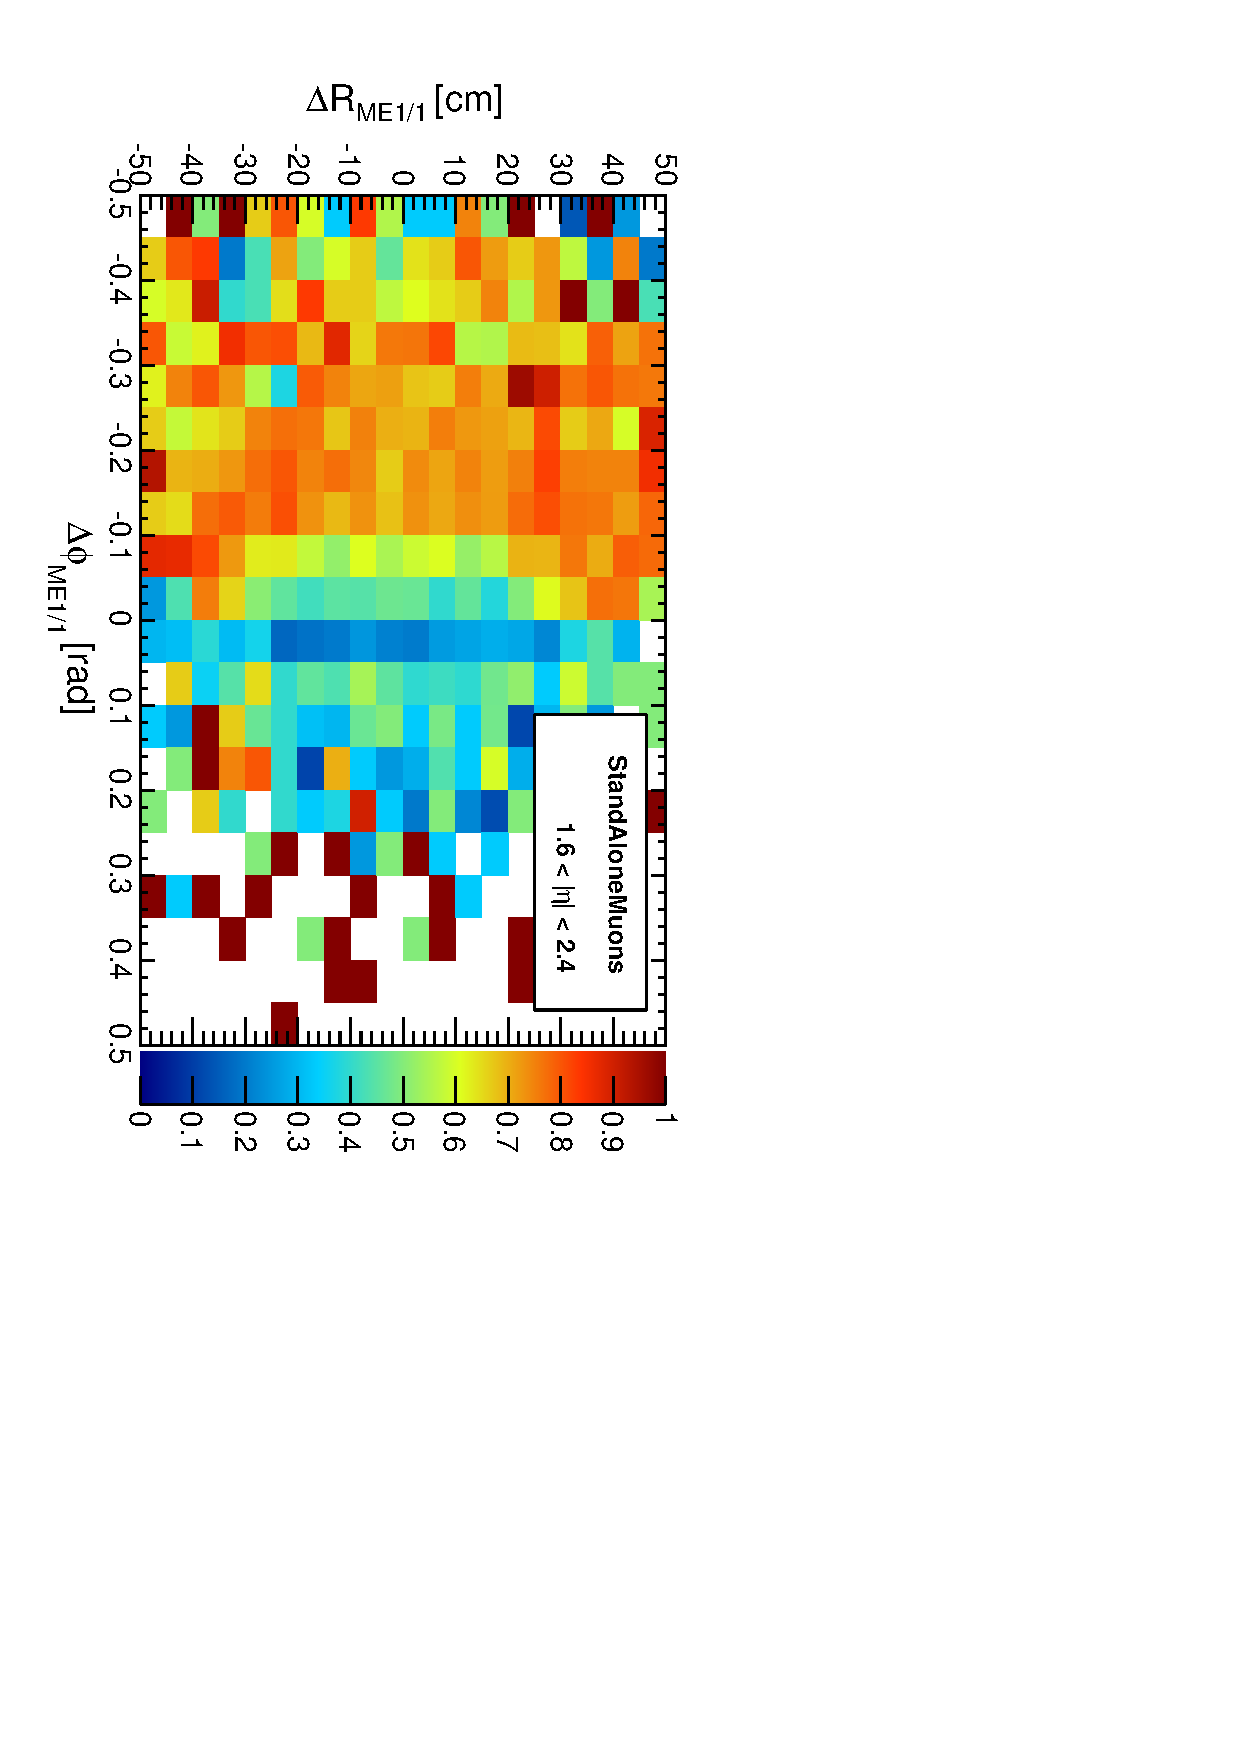
\includegraphics[height=0.5\linewidth, angle=90]{me11_StandAloneUpdatedDefault.pdf}
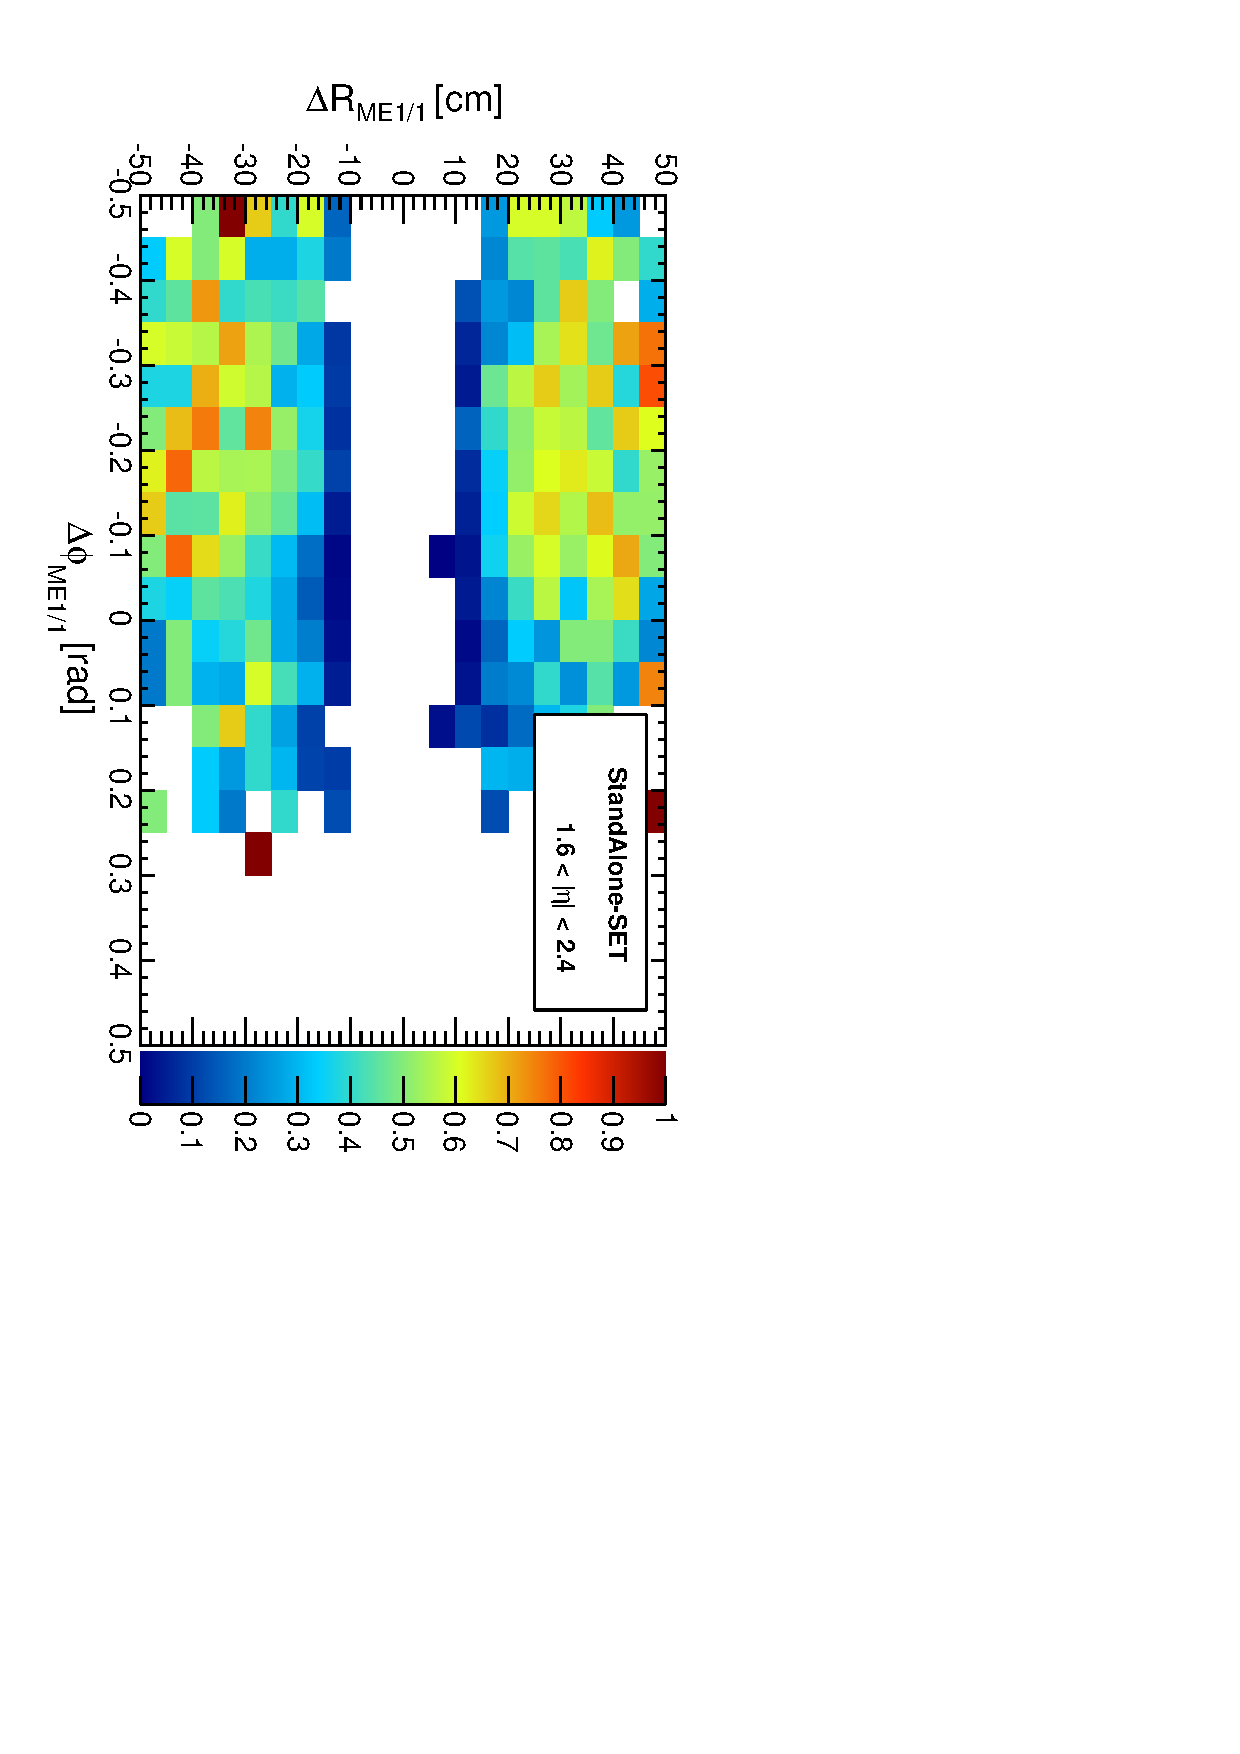
\includegraphics[height=0.5\linewidth, angle=90]{me11_StandAloneUpdatedSET.pdf}
\end{frame}

\begin{frame}
\frametitle{Separation in muon endcap}
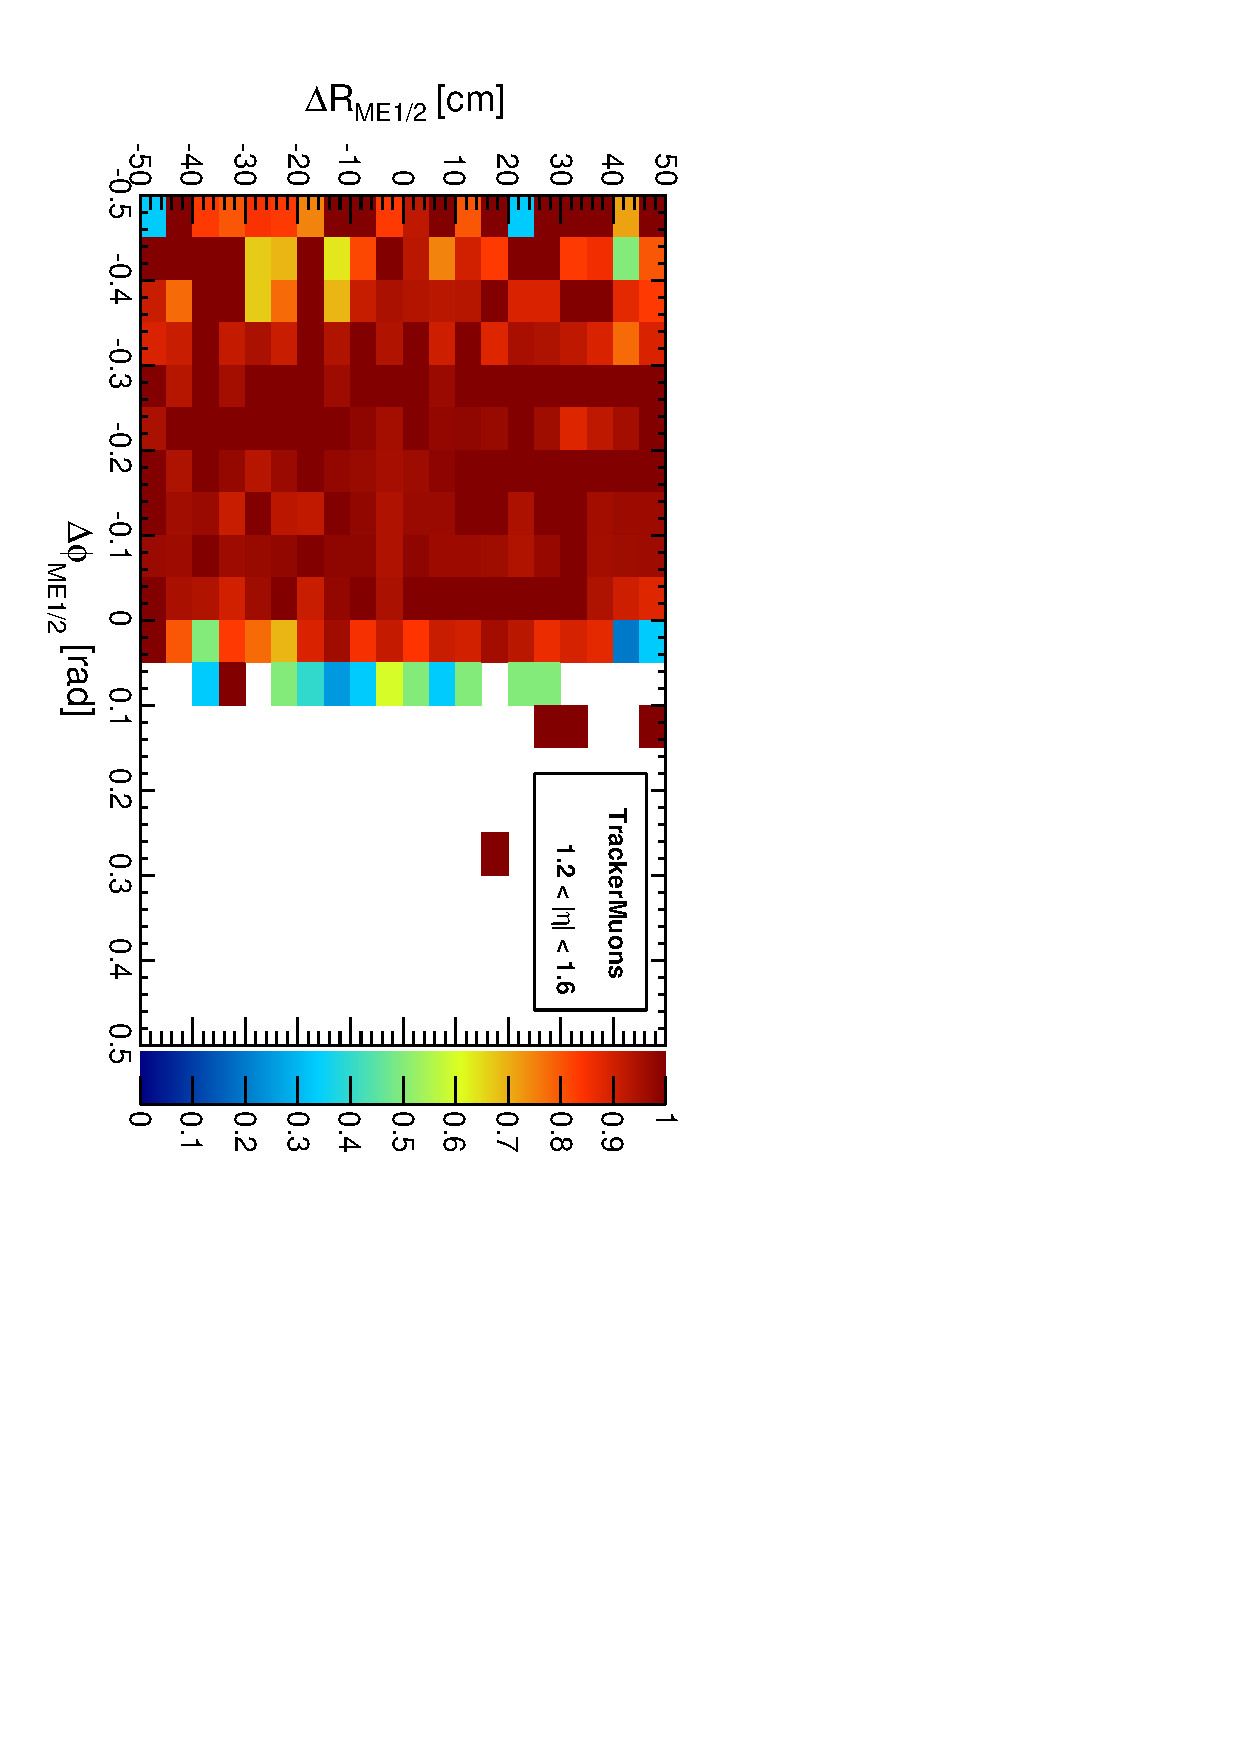
\includegraphics[height=0.5\linewidth, angle=90]{me12_TrackerMuons.pdf}
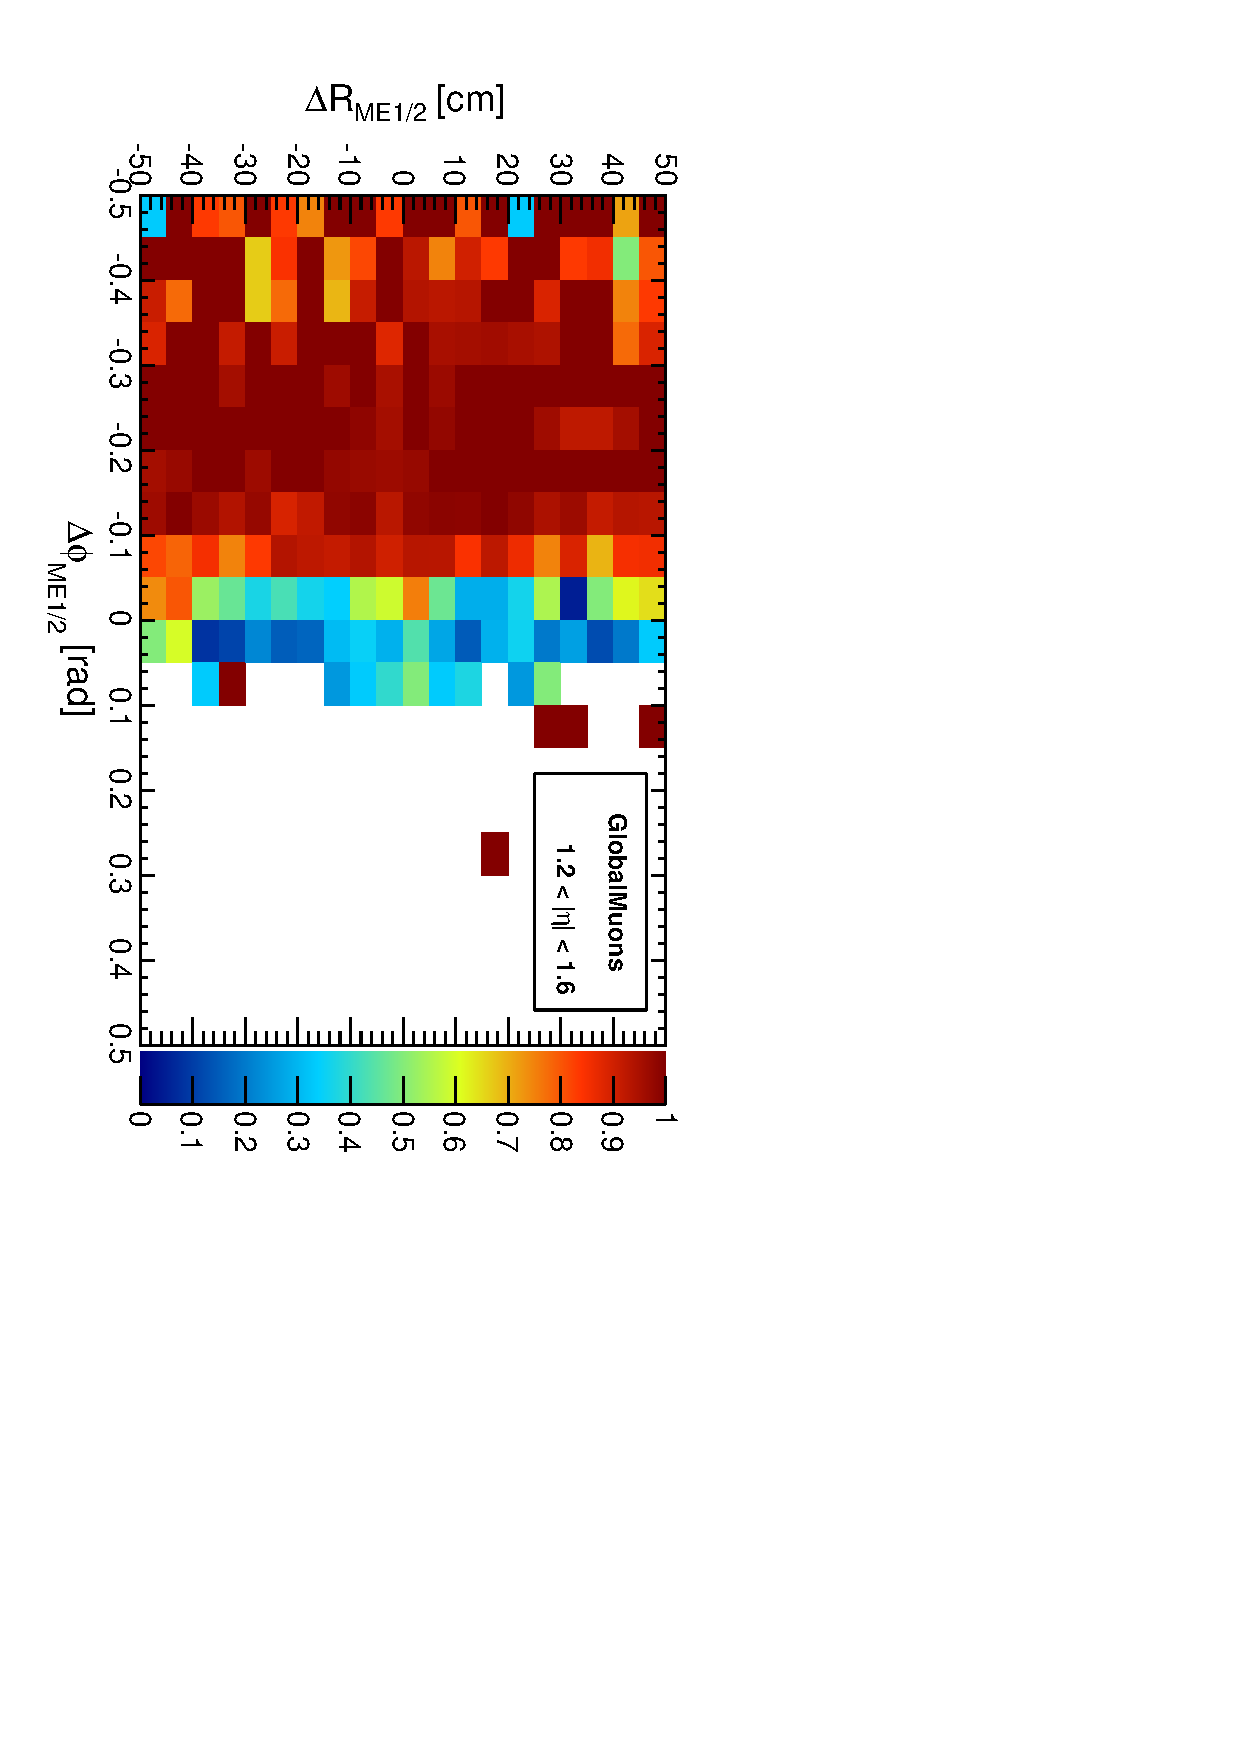
\includegraphics[height=0.5\linewidth, angle=90]{me12_GlobalMuons.pdf}

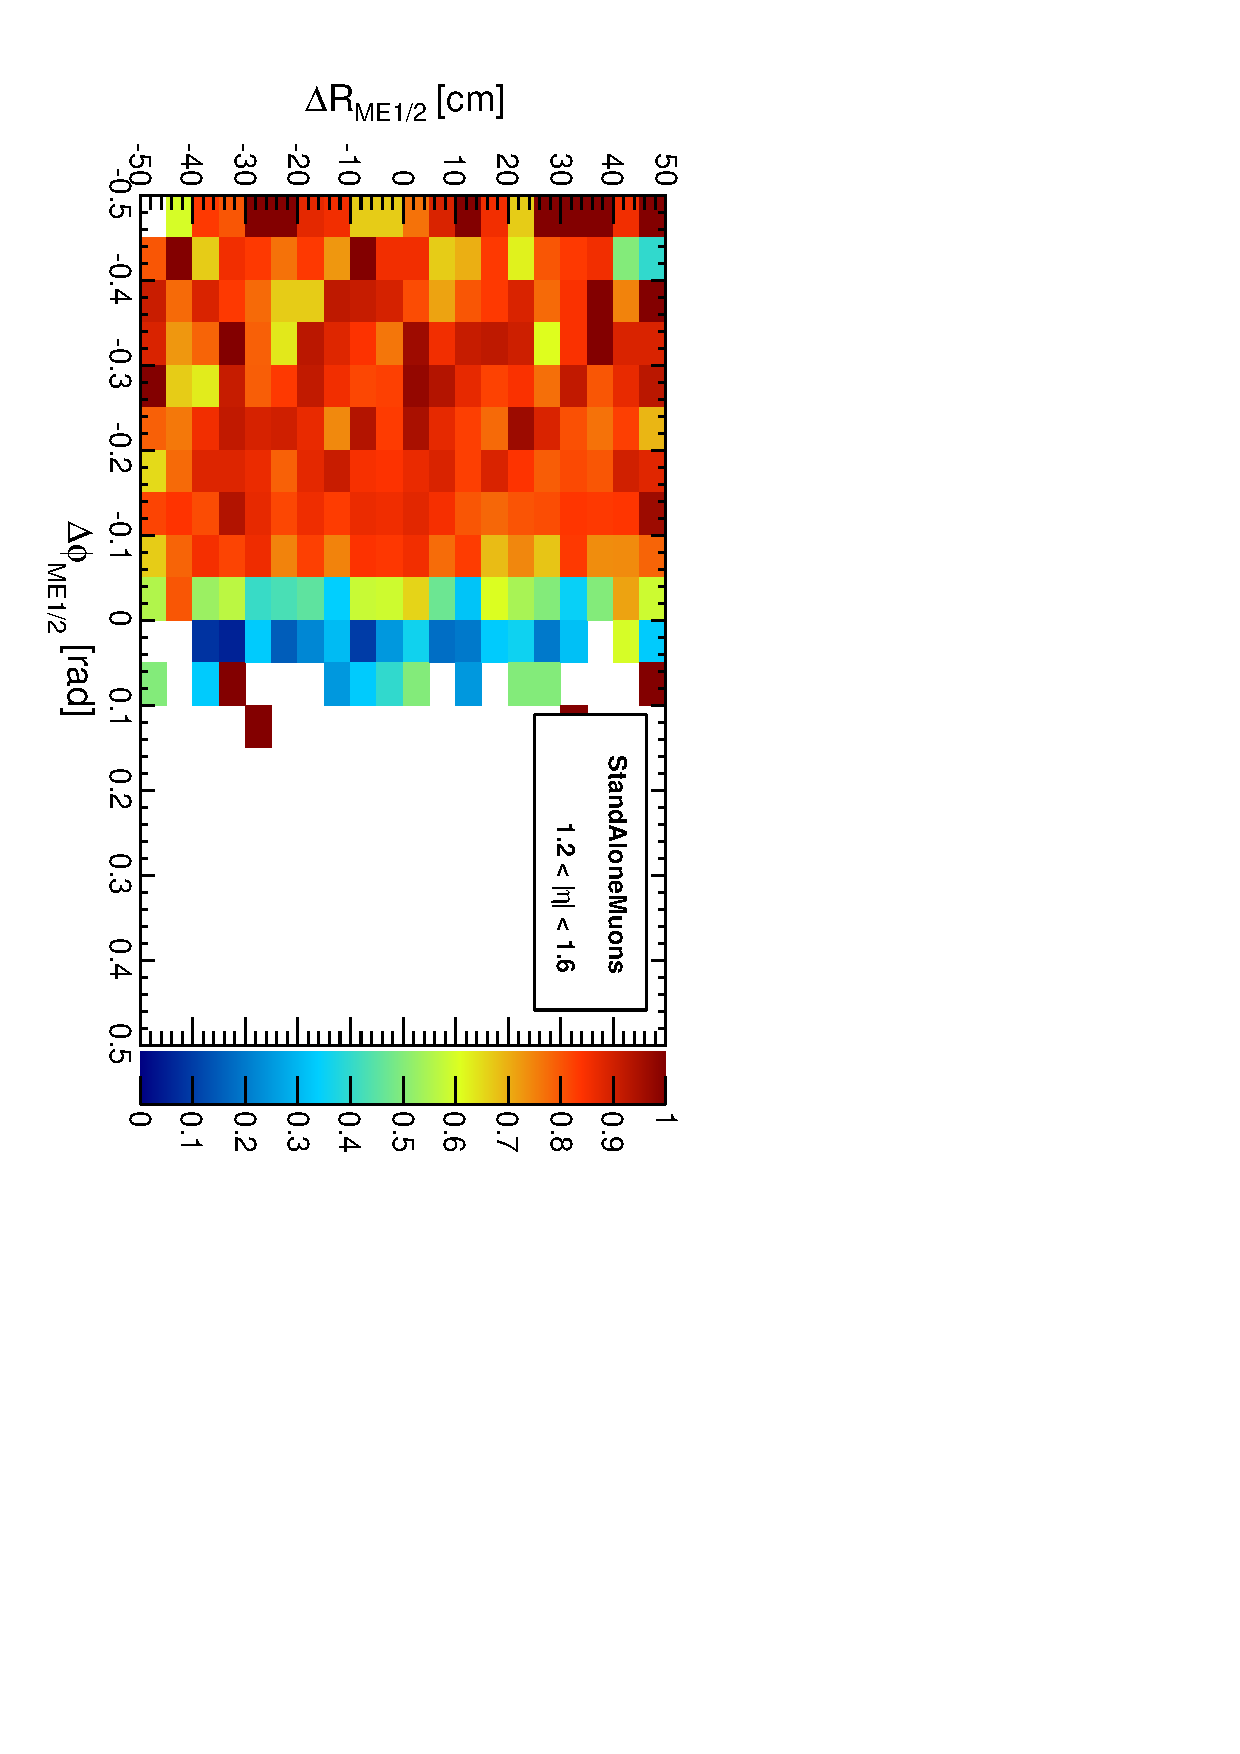
\includegraphics[height=0.5\linewidth, angle=90]{me12_StandAloneUpdatedDefault.pdf}
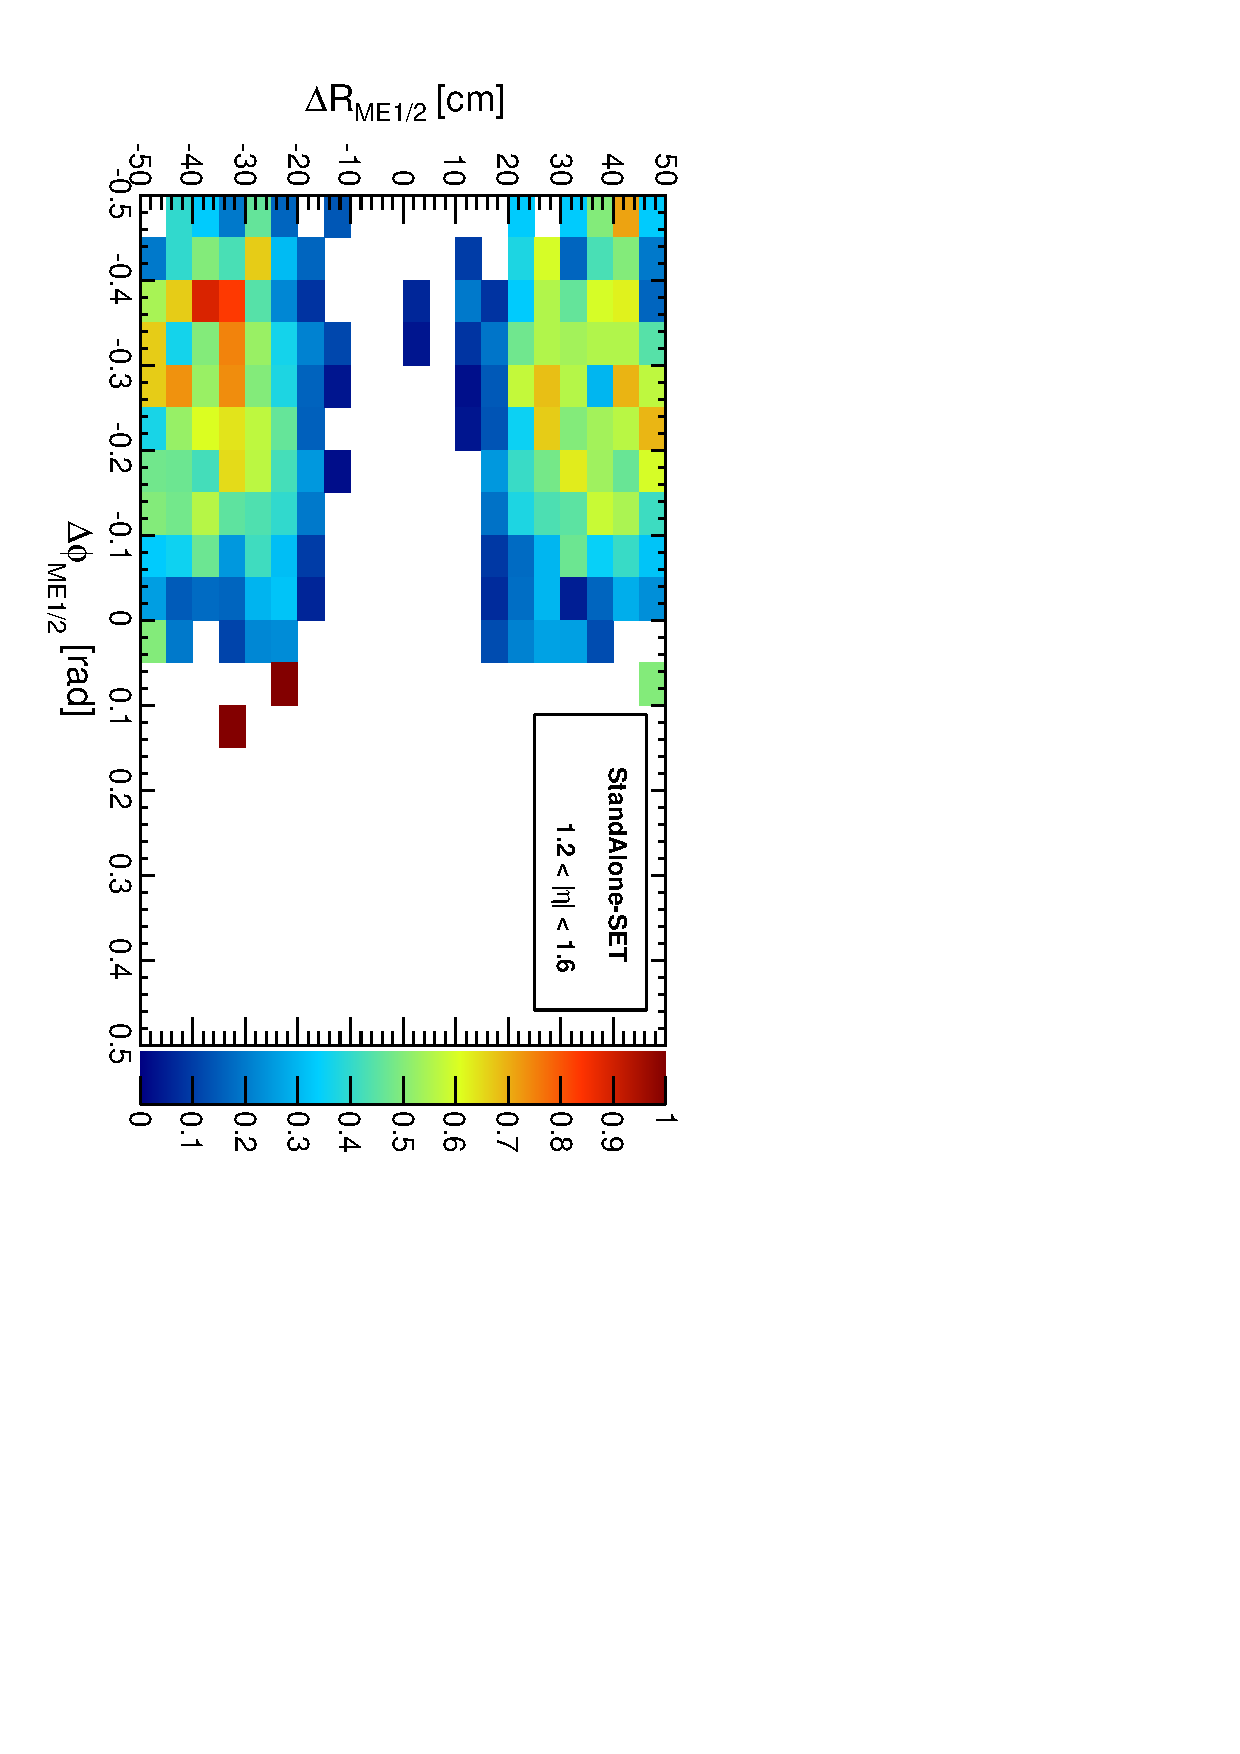
\includegraphics[height=0.5\linewidth, angle=90]{me12_StandAloneUpdatedSET.pdf}

I'm not really satisfied with these yet--- we need to understand why
they're not more completely illuminated (and maybe generate some
dimuon guns which would cover more, to tell us the whole story)
\end{frame}

\begin{frame}
\frametitle{Trigger efficiency\only<2>{: barrel}\only<3>{: endcap}}

Denominator: \only<1>{$\eta_1 < 2.4$}\only<2>{$\eta_1 < 1.0$ (barrel)}\only<3>{$1.0 < \eta_1 < 2.4$ (endcap)}; efficiency for triggering \only<1>{as a function of $p_T$}

\vfill
$pT_1$ is highest $p_T$, driving trigger-efficiency, $pT_2$ is second-highest, driving reconstruction-efficiency (both evaluated at generator-level)

\vfill
\only<1>{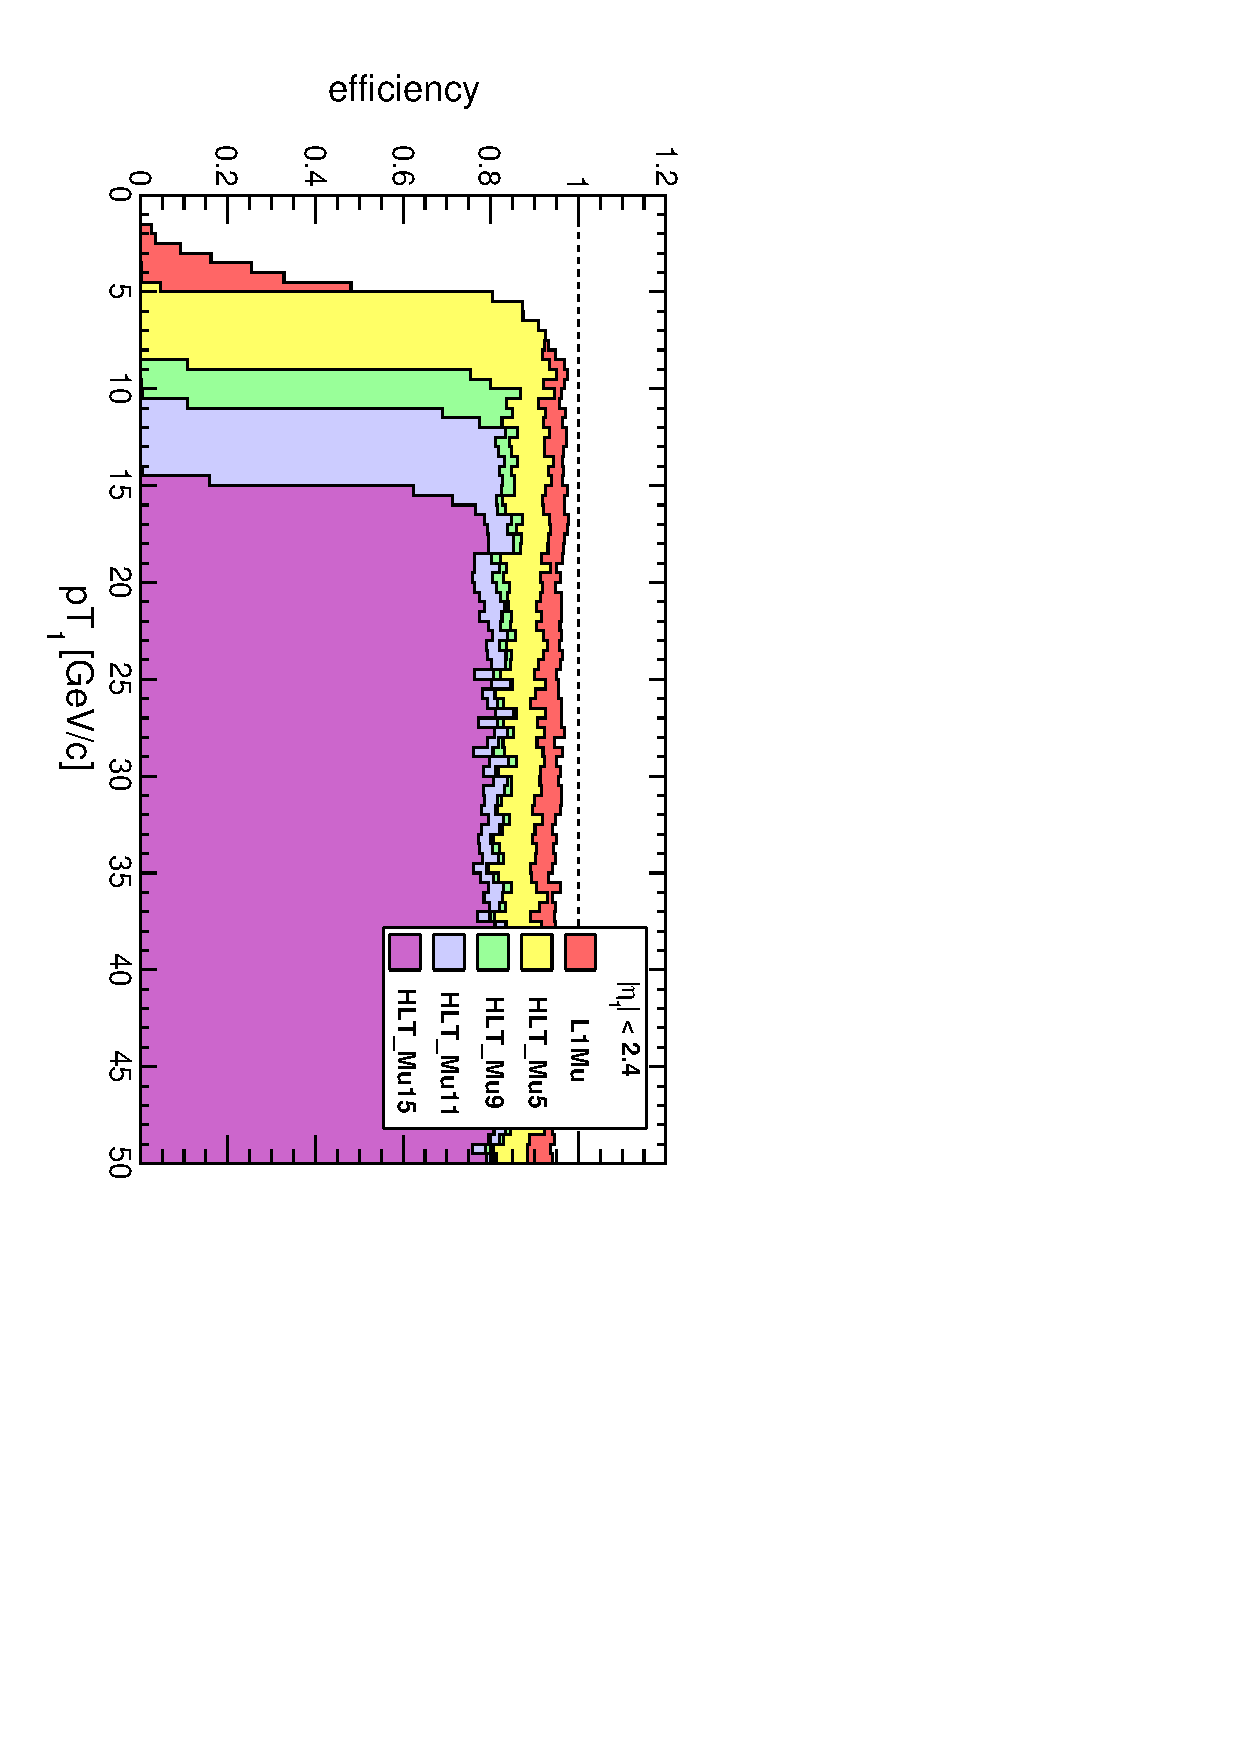
\includegraphics[height=0.5\linewidth, angle=90]{triggereta24_p1.pdf}
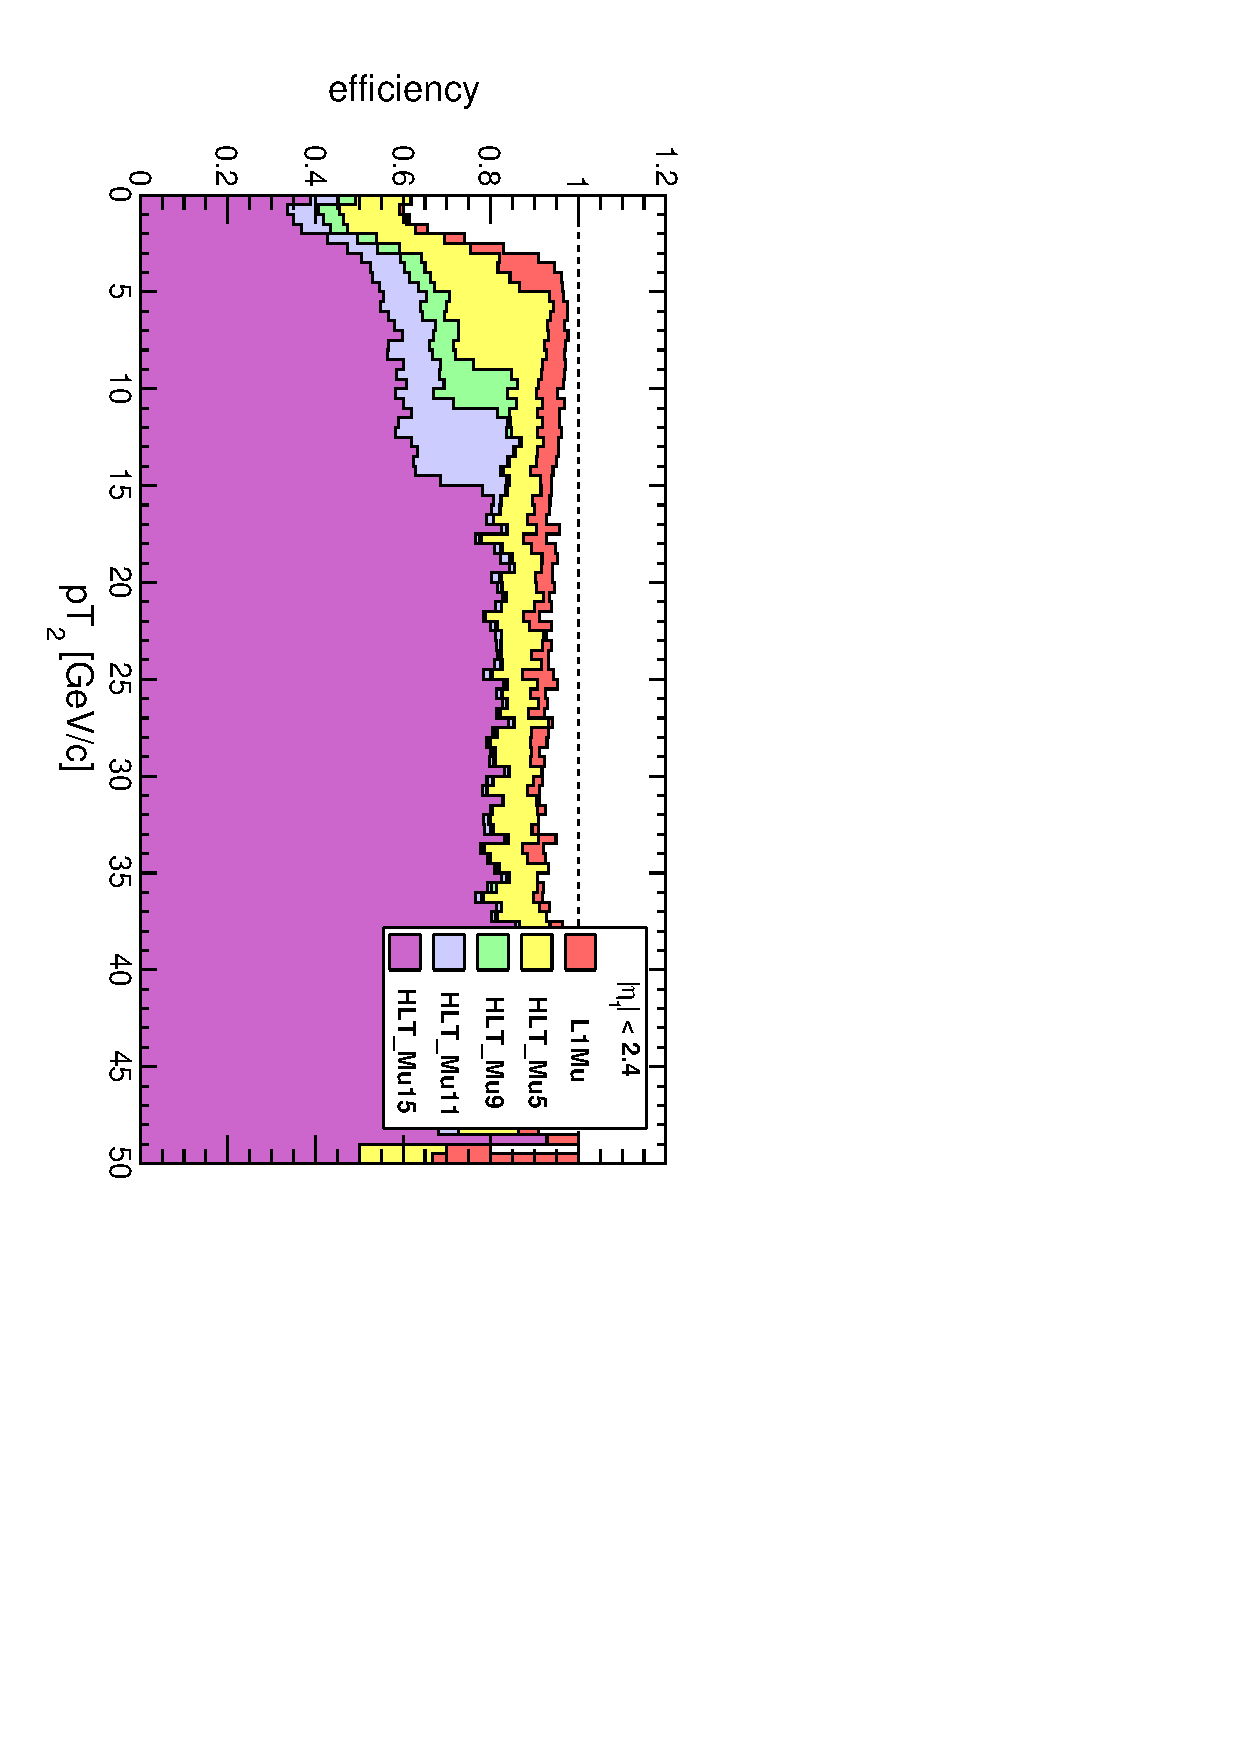
\includegraphics[height=0.5\linewidth, angle=90]{triggereta24_p2.pdf}}

\only<2>{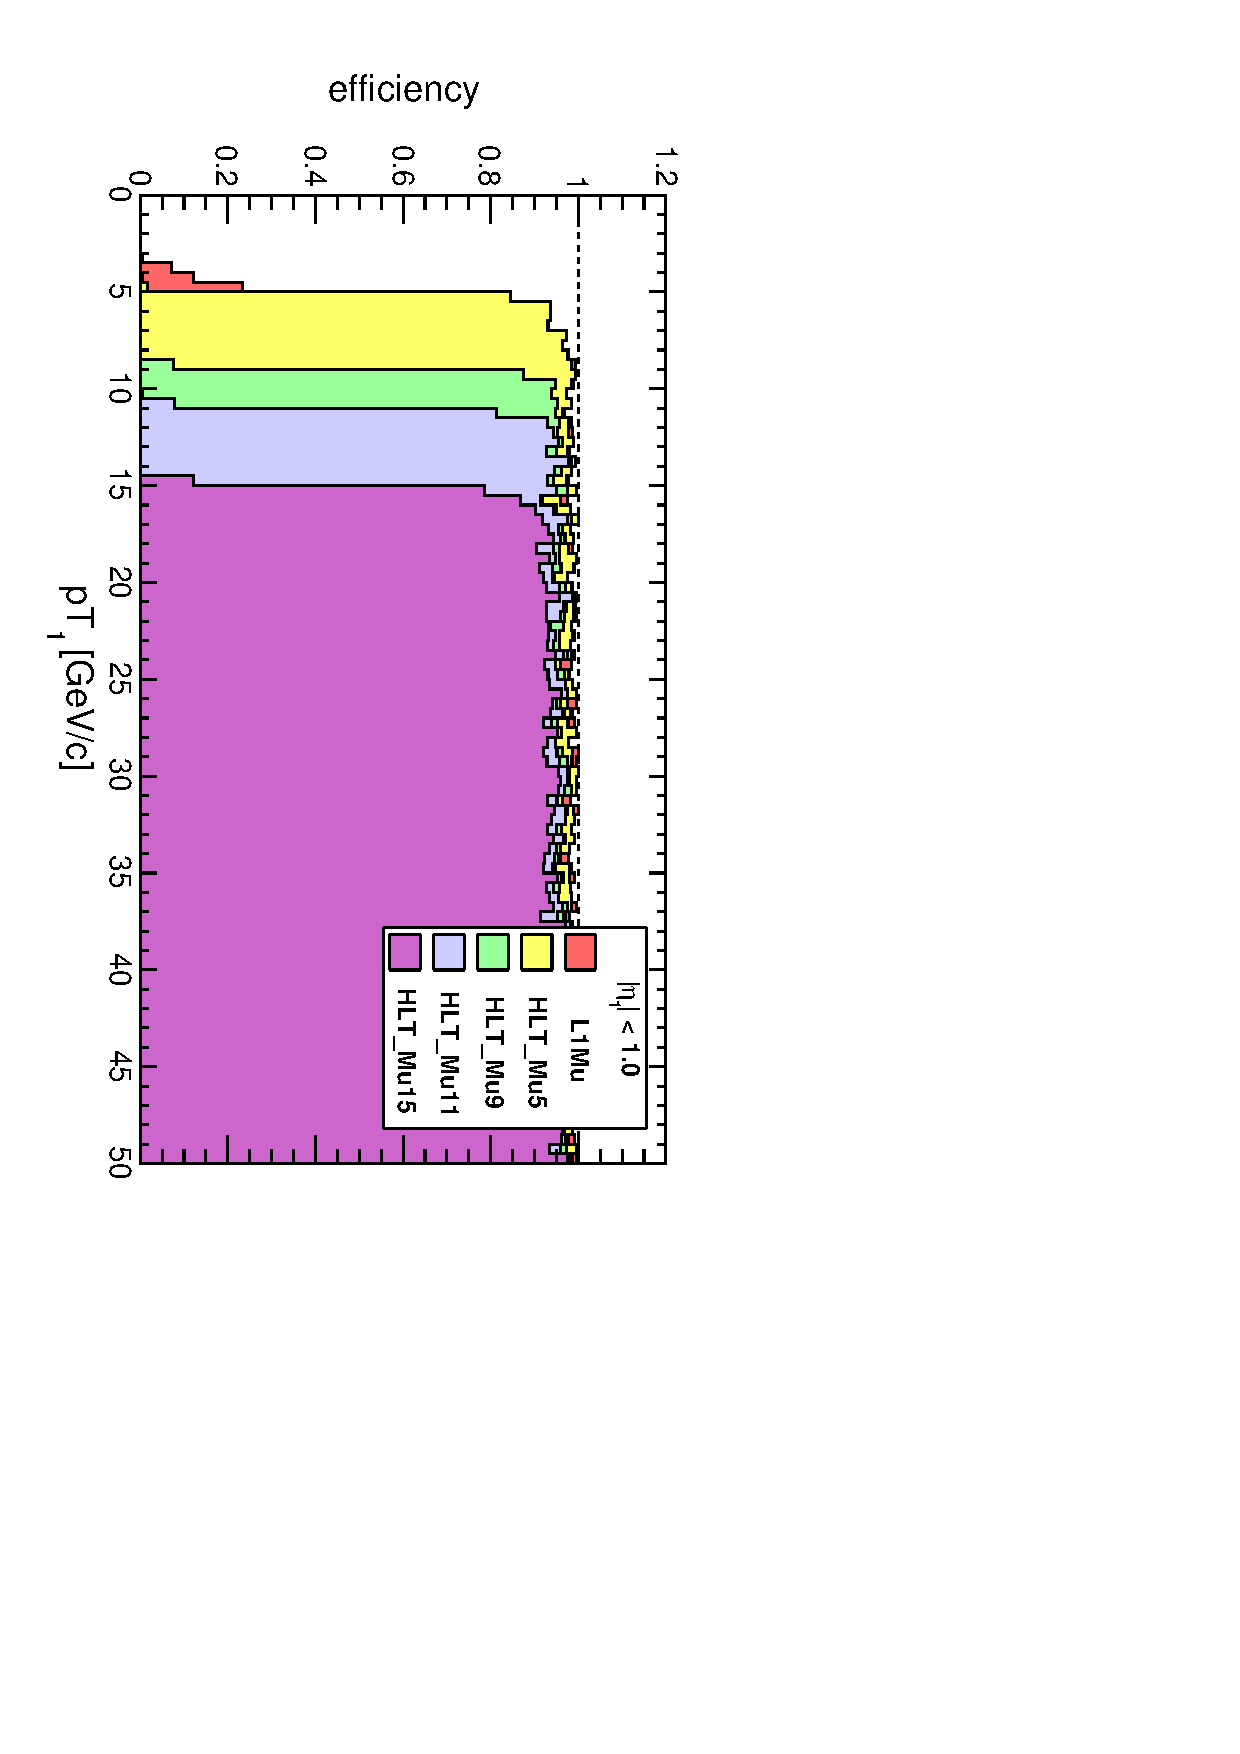
\includegraphics[height=0.5\linewidth, angle=90]{triggereta10_p1.pdf}
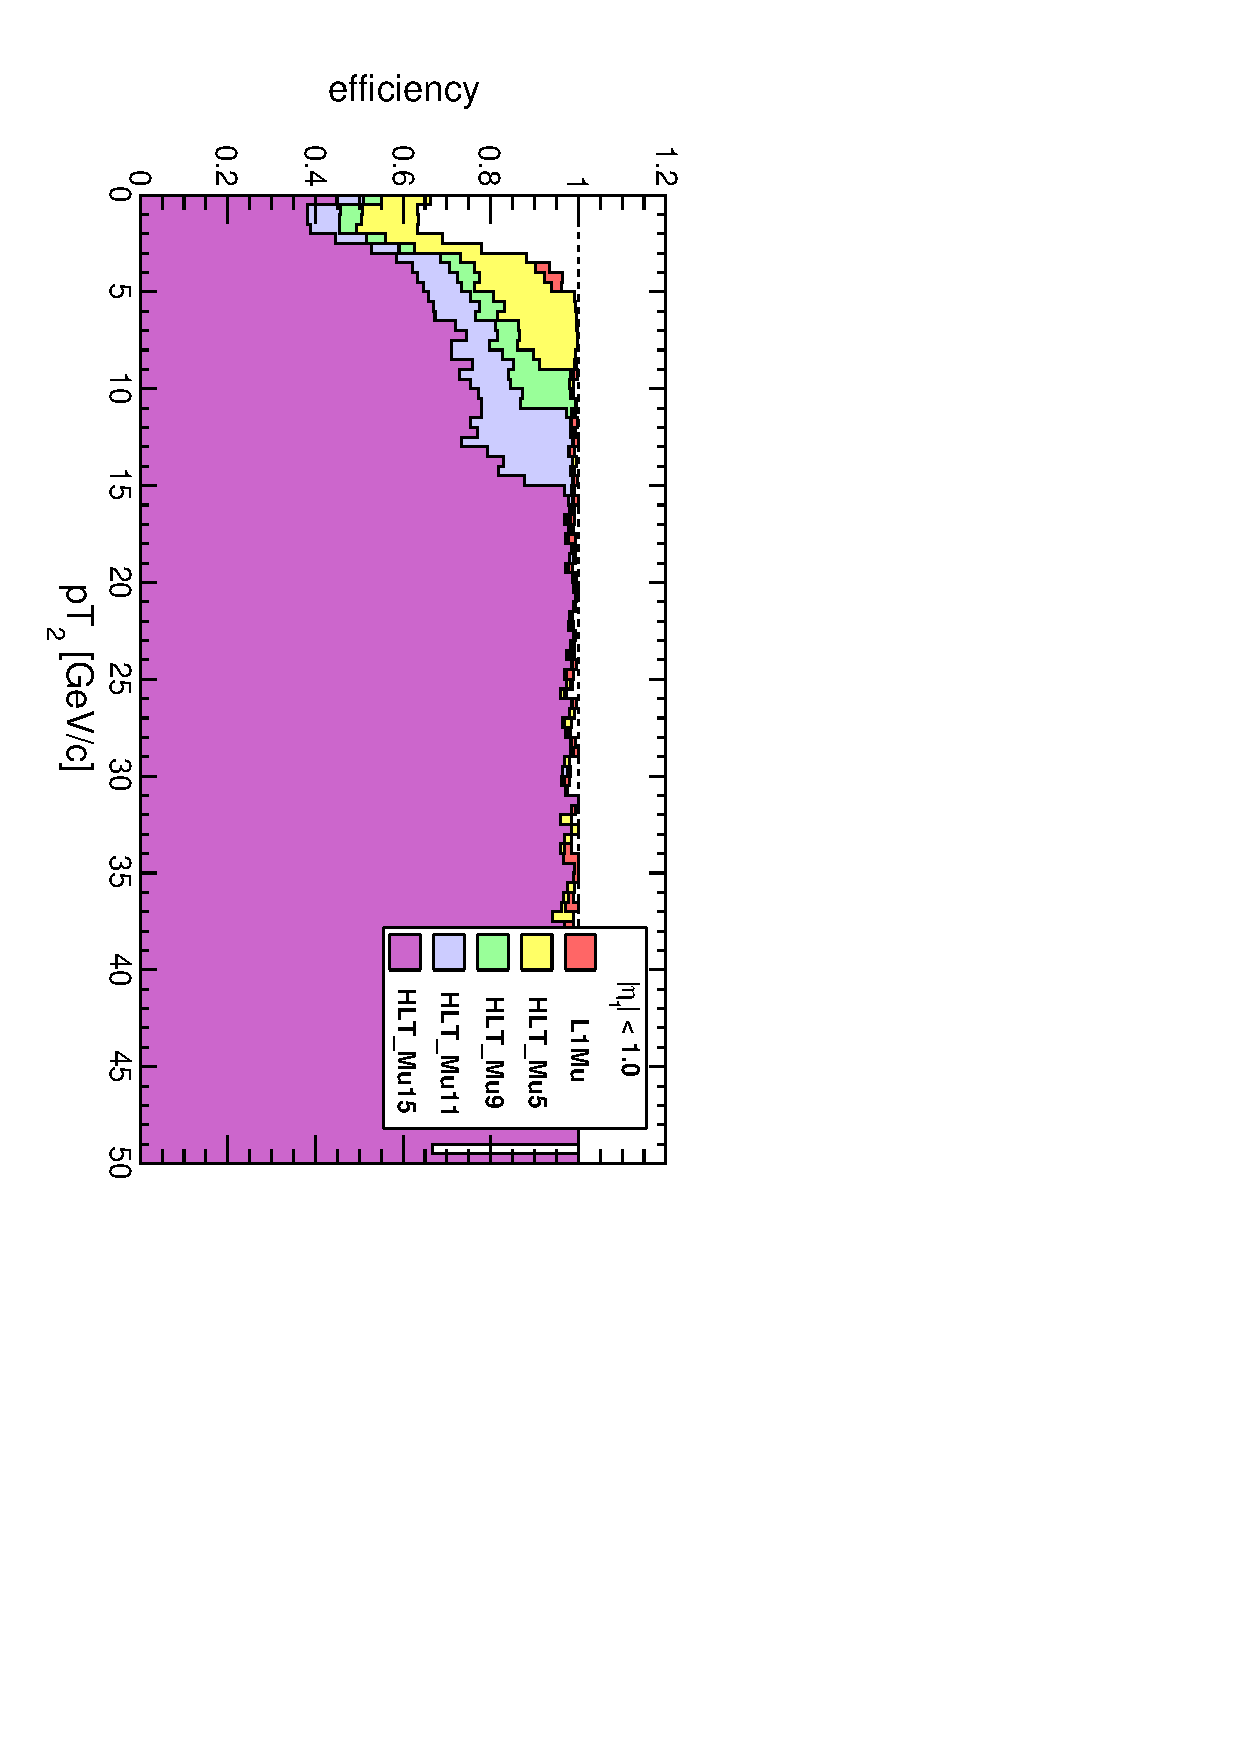
\includegraphics[height=0.5\linewidth, angle=90]{triggereta10_p2.pdf}}

\only<3>{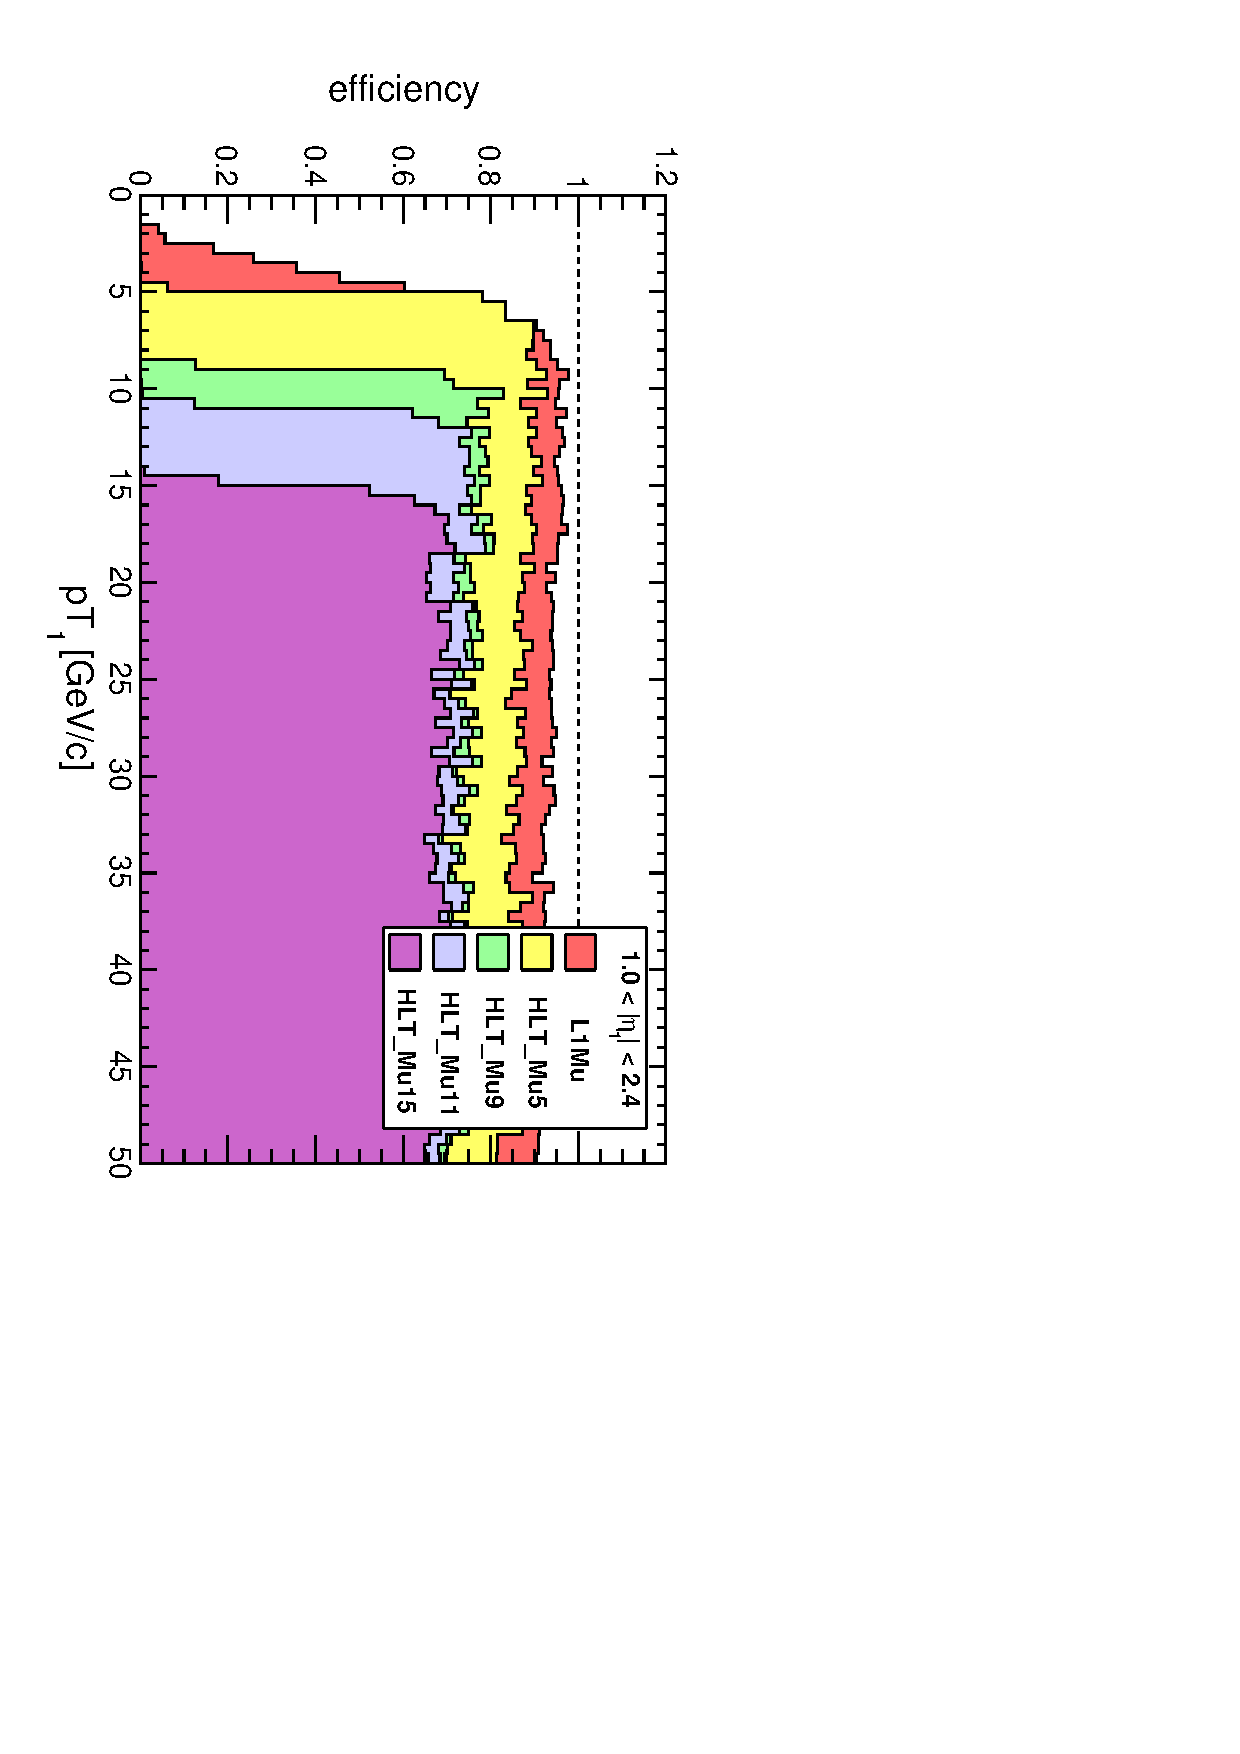
\includegraphics[height=0.5\linewidth, angle=90]{triggeretaendcap_p1.pdf}
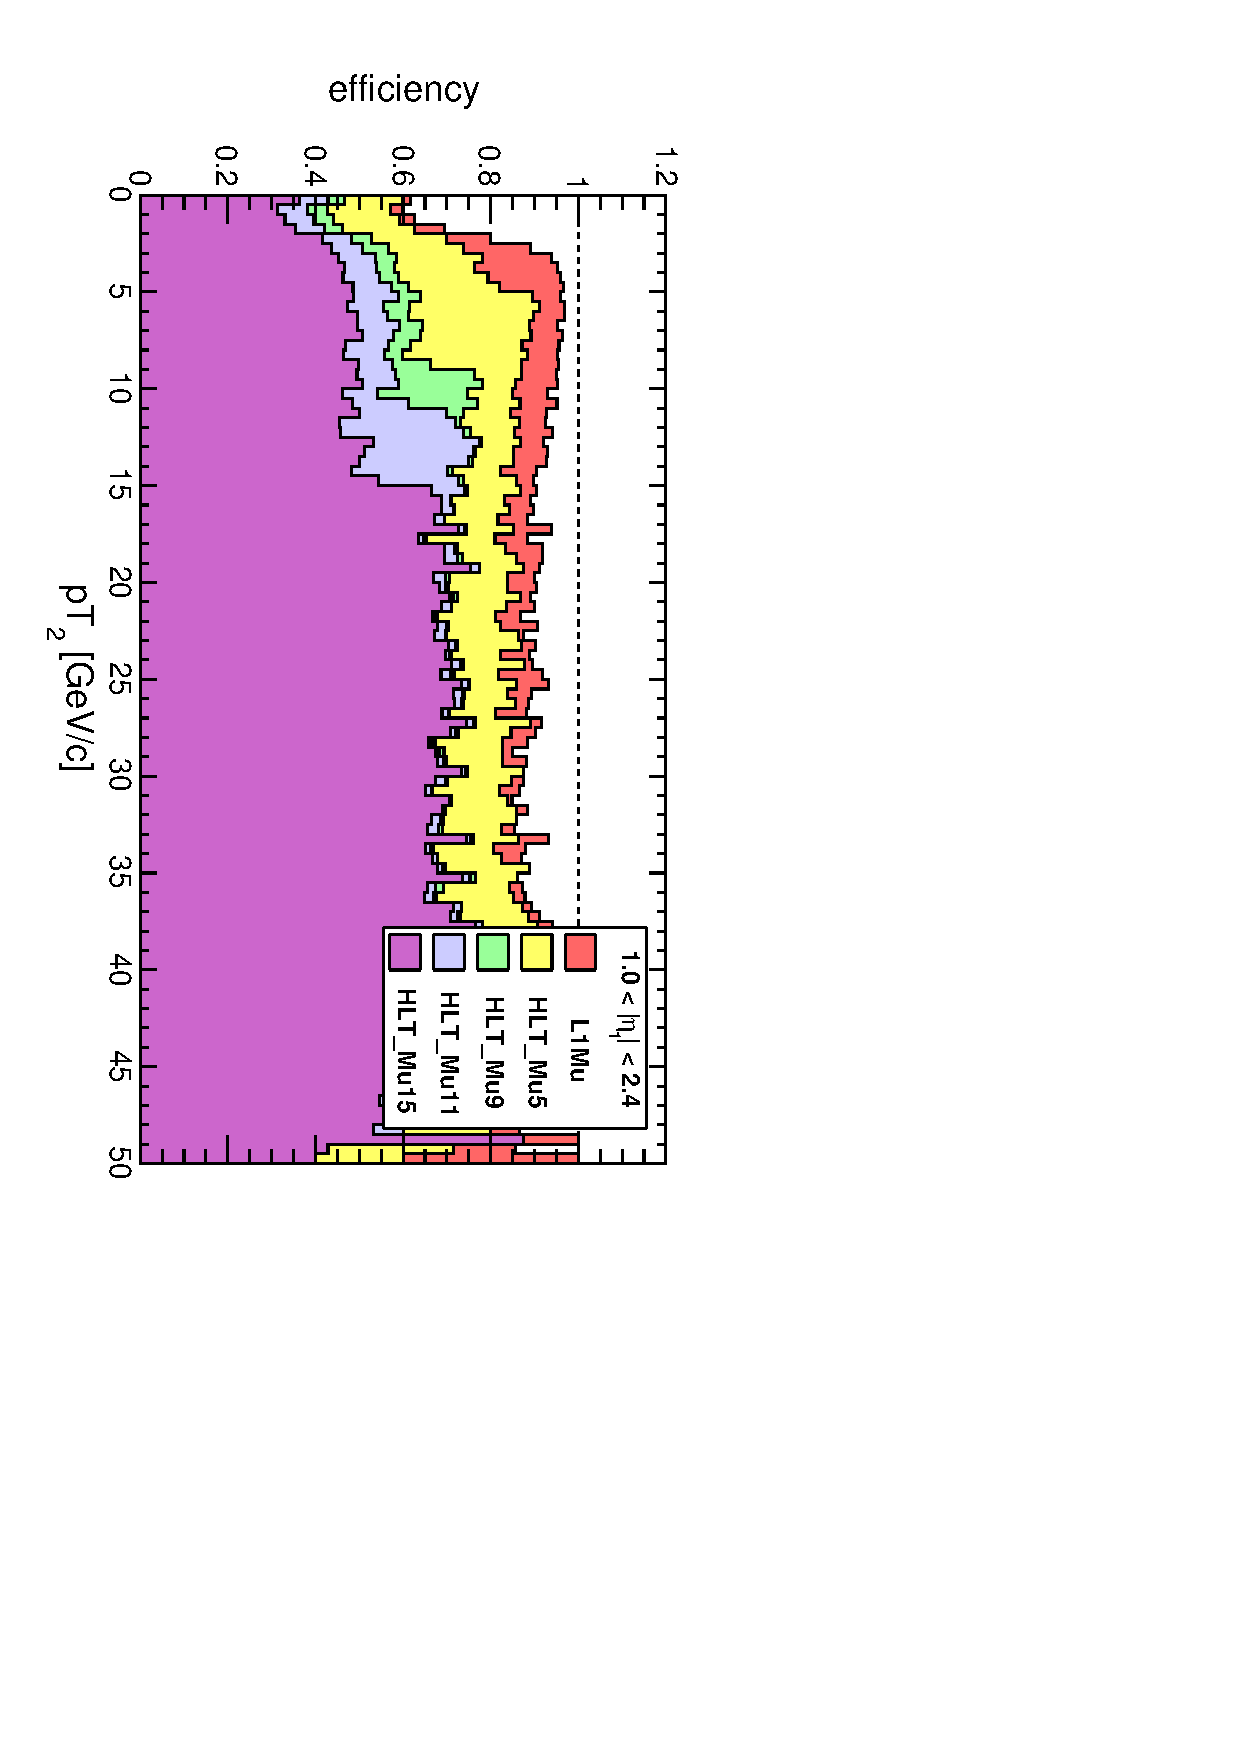
\includegraphics[height=0.5\linewidth, angle=90]{triggeretaendcap_p2.pdf}}

\vfill Is the L1Mu going below the HLT\_Mu5 curve?  It looks like it.
I had thought that L1Mu was a prerequisite for HLT\_Mu5 {\small
  (according to ConfDB, ``L1SingleMu3'' is a prerequisite for HLT\_Mu5, but L1Mu is
  ``L1SingleMu3 OR L1SingleMu7'')}
\end{frame}

\begin{frame}
\frametitle{Merging efficiency}
Assuming that we have reconstructed both TrackerMuons (denominator),
what is the efficiency of grouping them in the same $\mu$-jet?

\vfill
\begin{columns}
\column{0.7\linewidth}

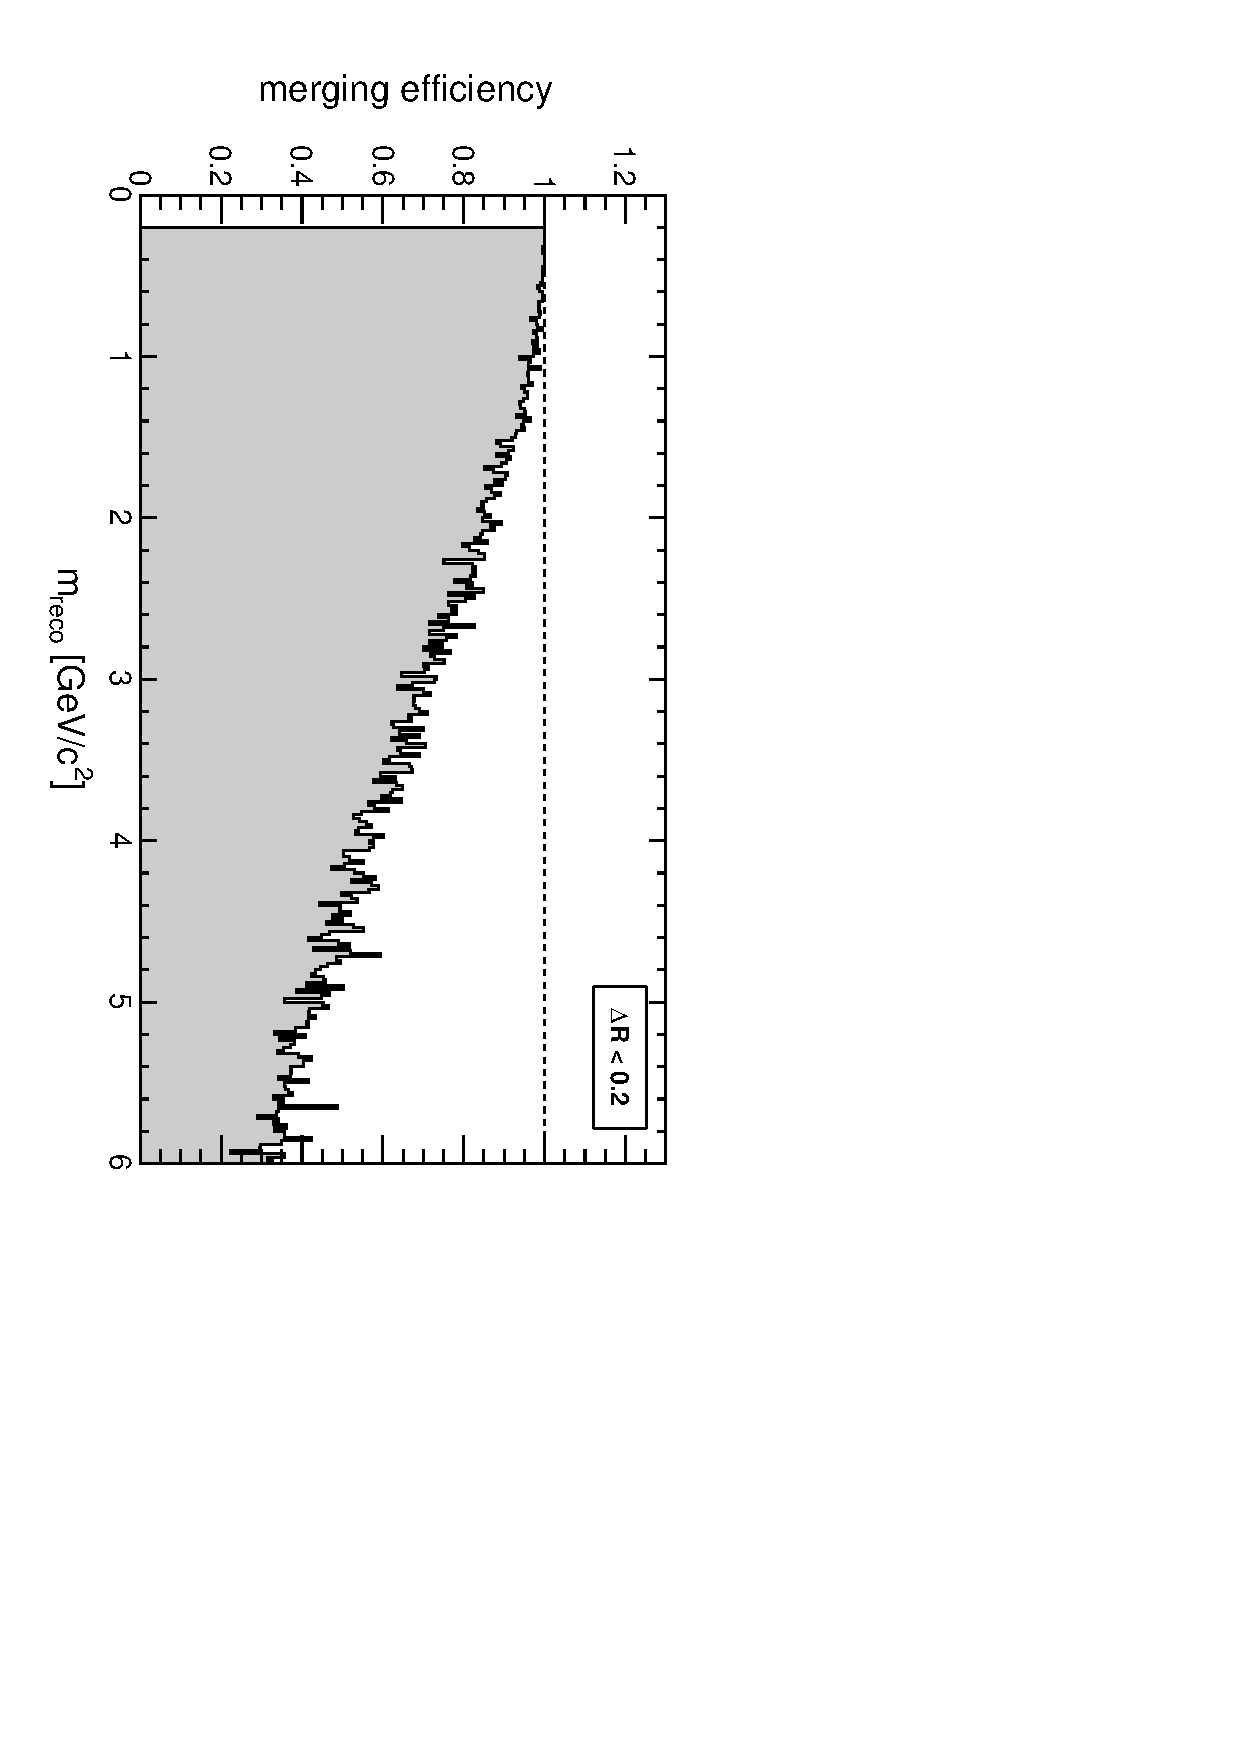
\includegraphics[height=0.5\linewidth, angle=90]{mergingeff_recomass_GroupByDeltaR.pdf}
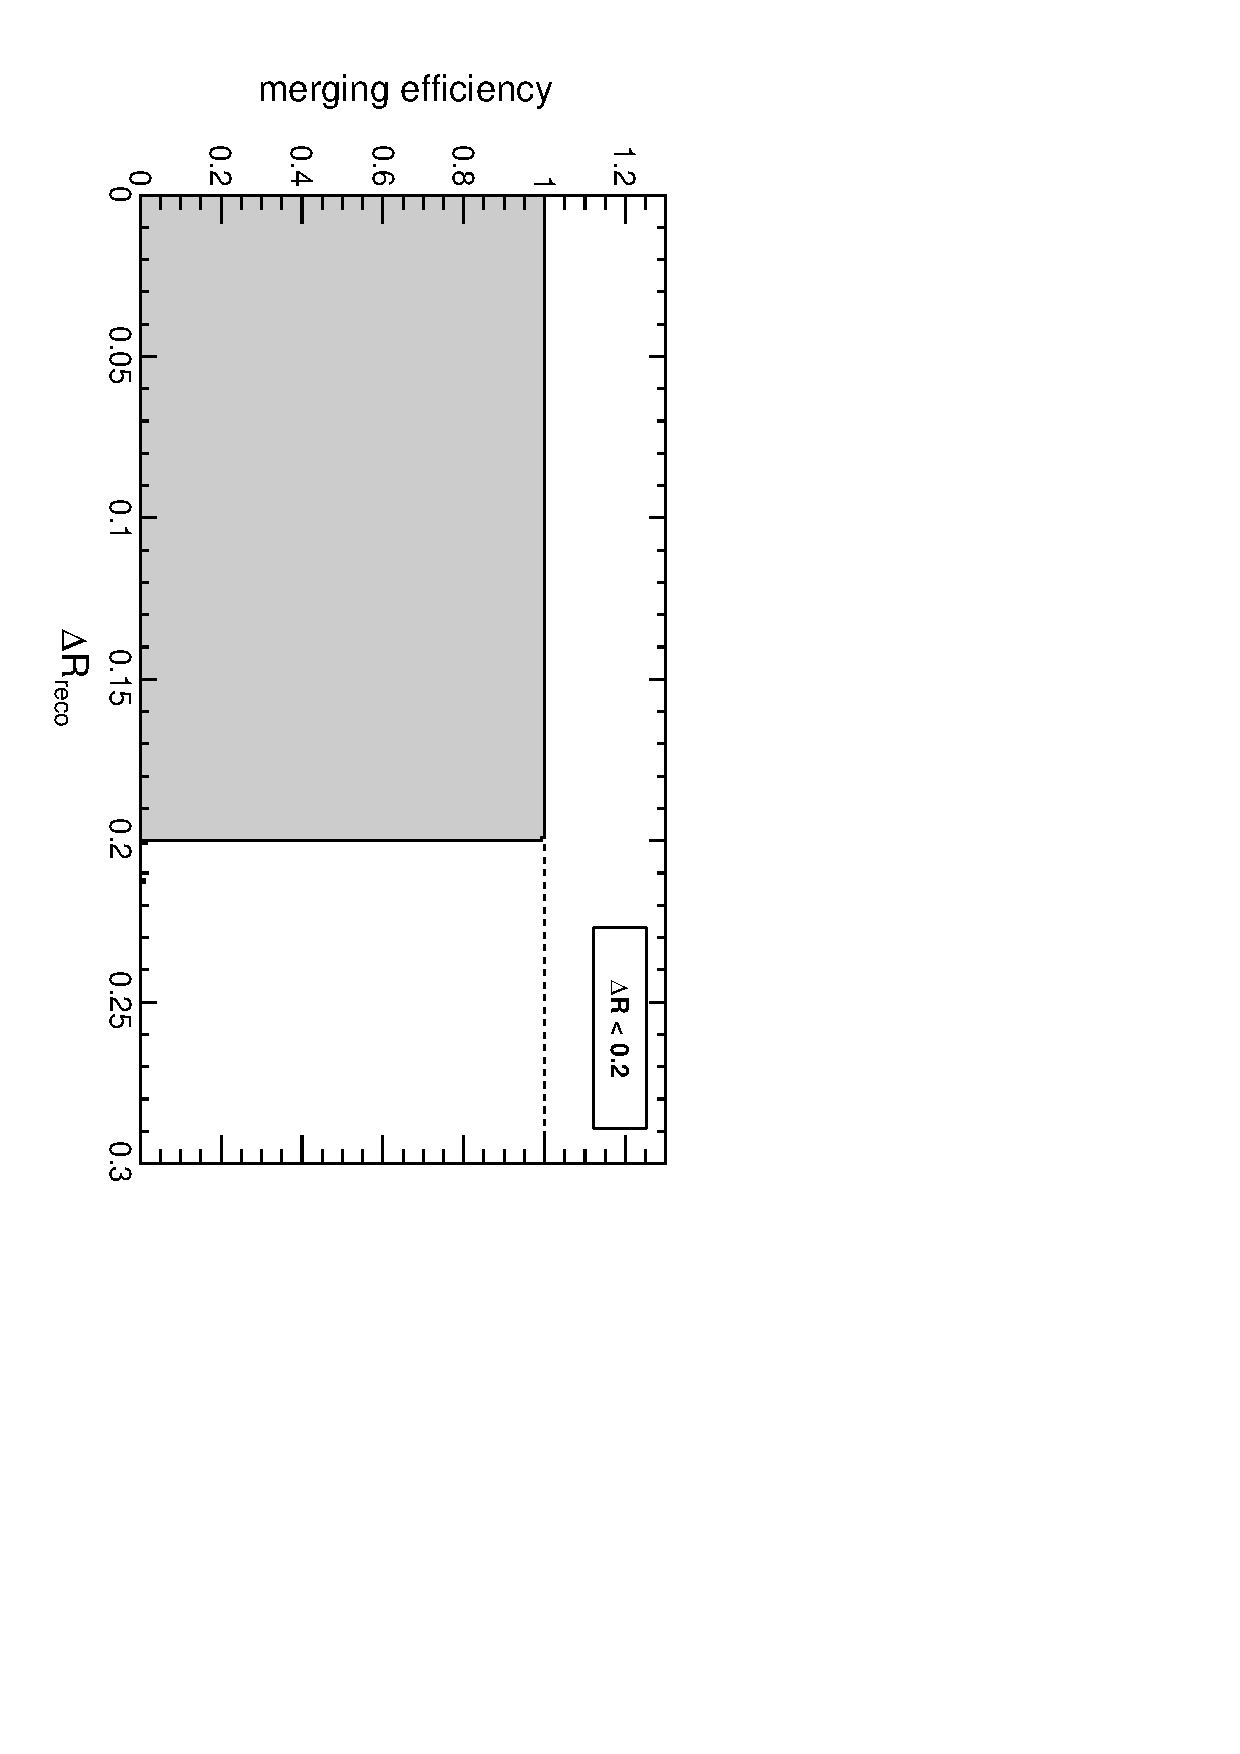
\includegraphics[height=0.5\linewidth, angle=90]{mergingeff_recodr_GroupByDeltaR.pdf}

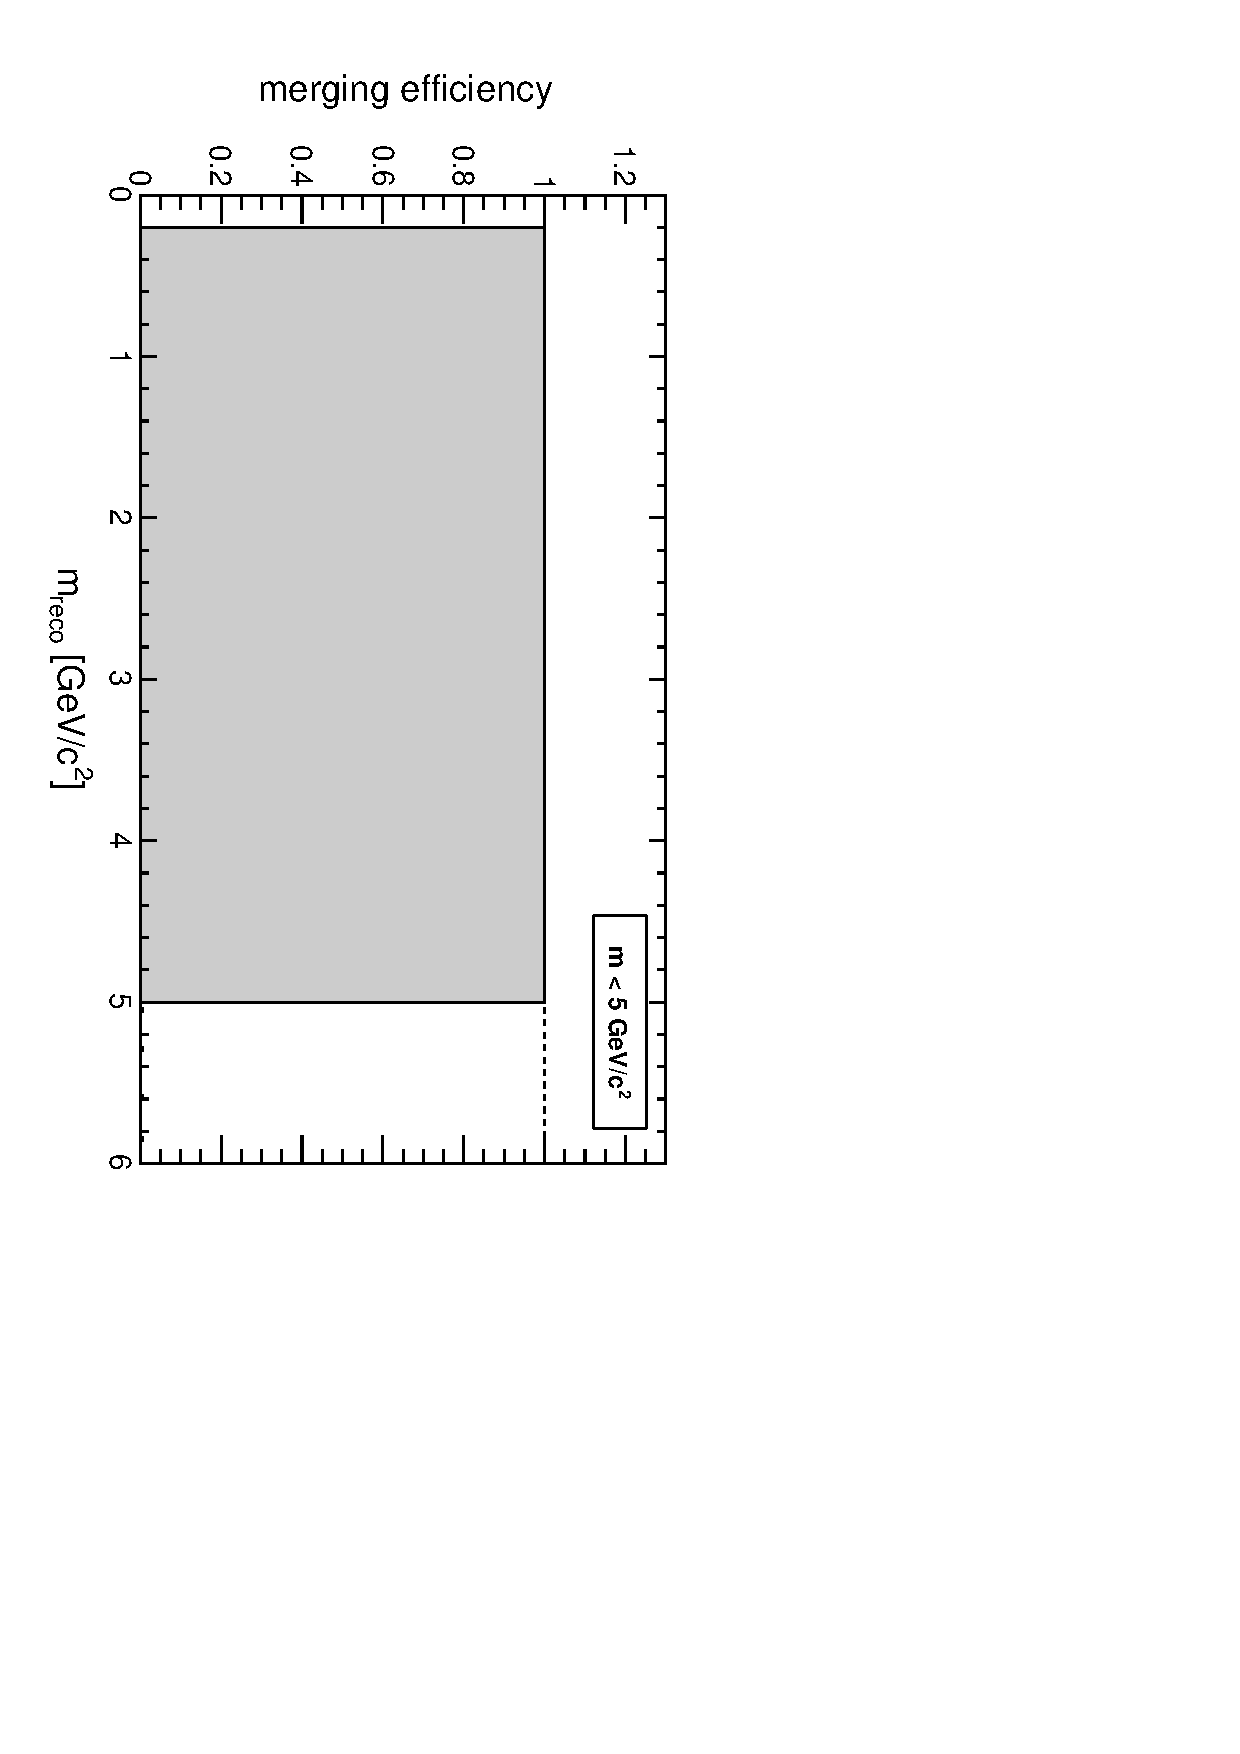
\includegraphics[height=0.5\linewidth, angle=90]{mergingeff_recomass_GroupByMass.pdf}
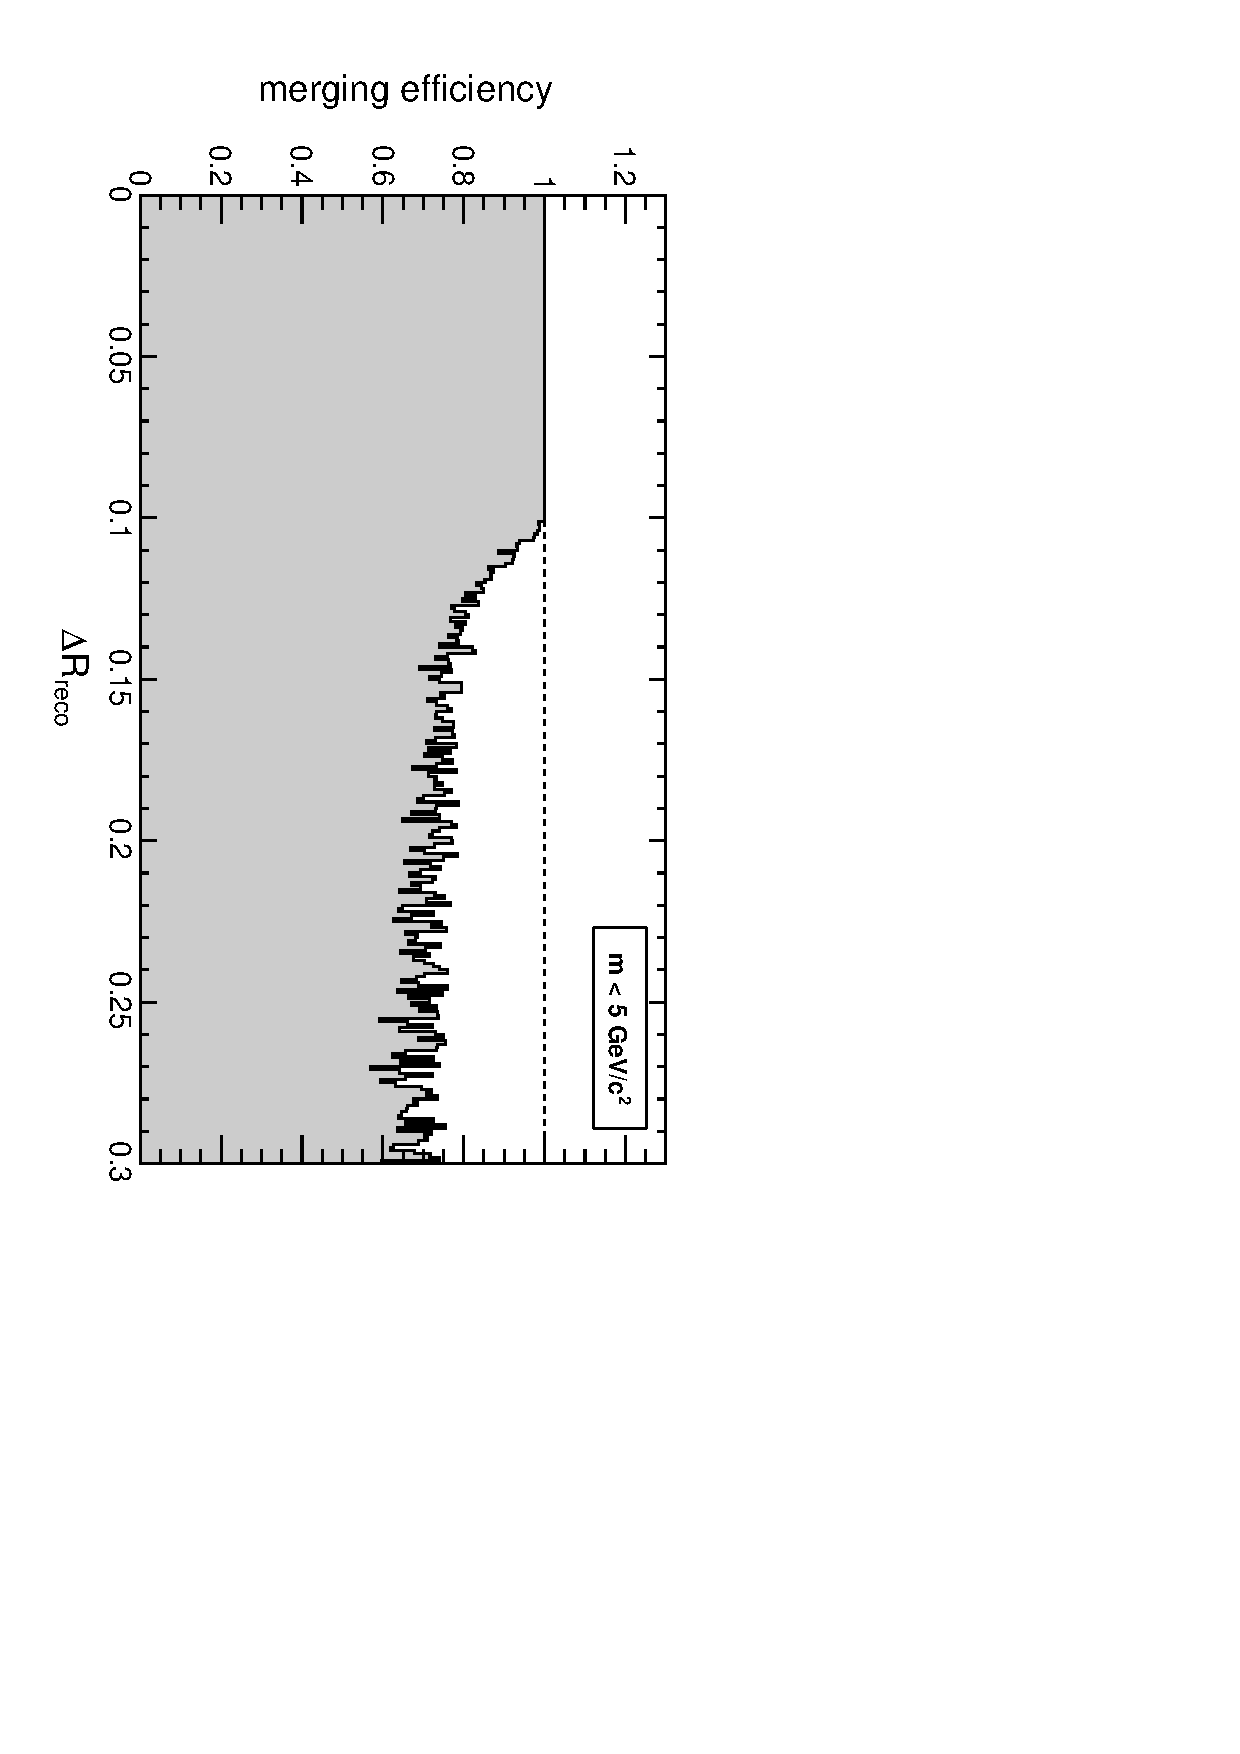
\includegraphics[height=0.5\linewidth, angle=90]{mergingeff_recodr_GroupByMass.pdf}

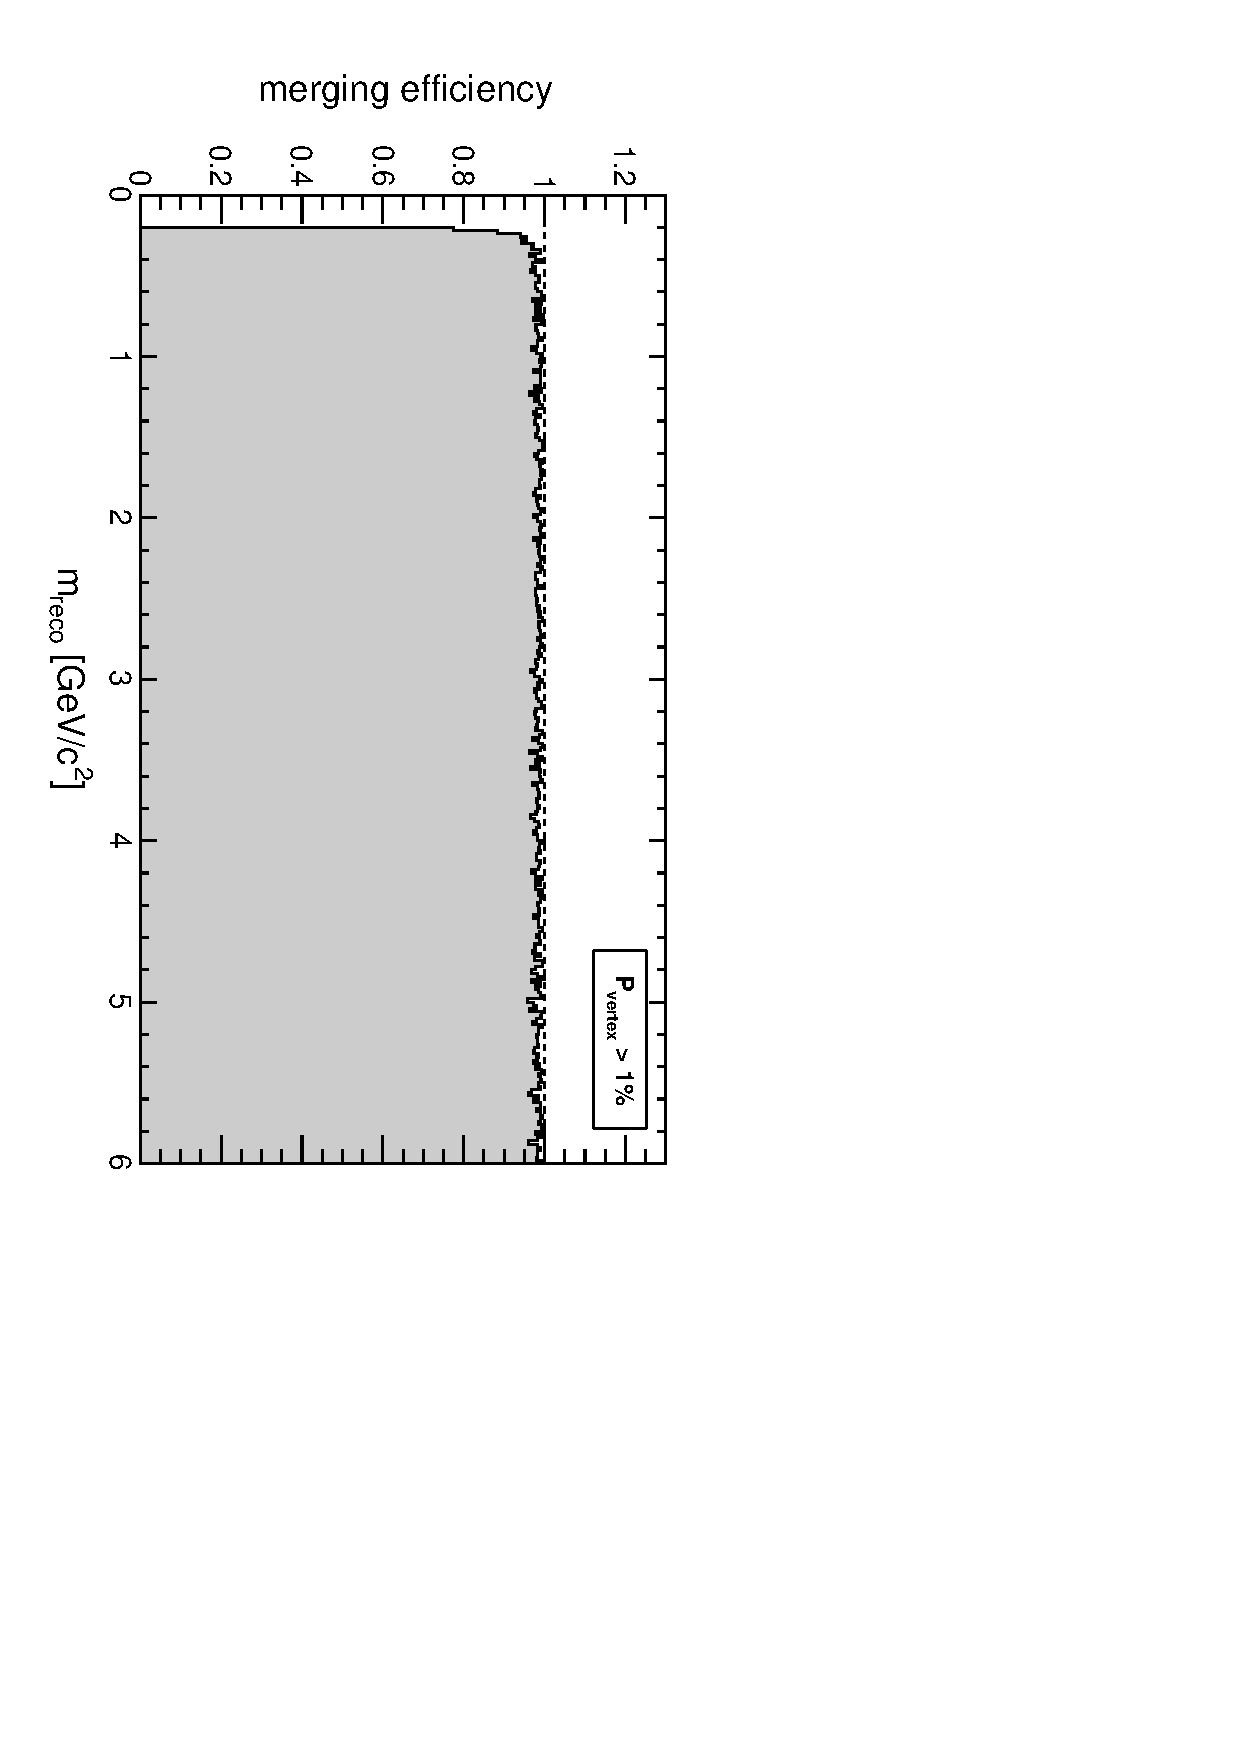
\includegraphics[height=0.5\linewidth, angle=90]{mergingeff_recomass_GroupByVertexProb.pdf}
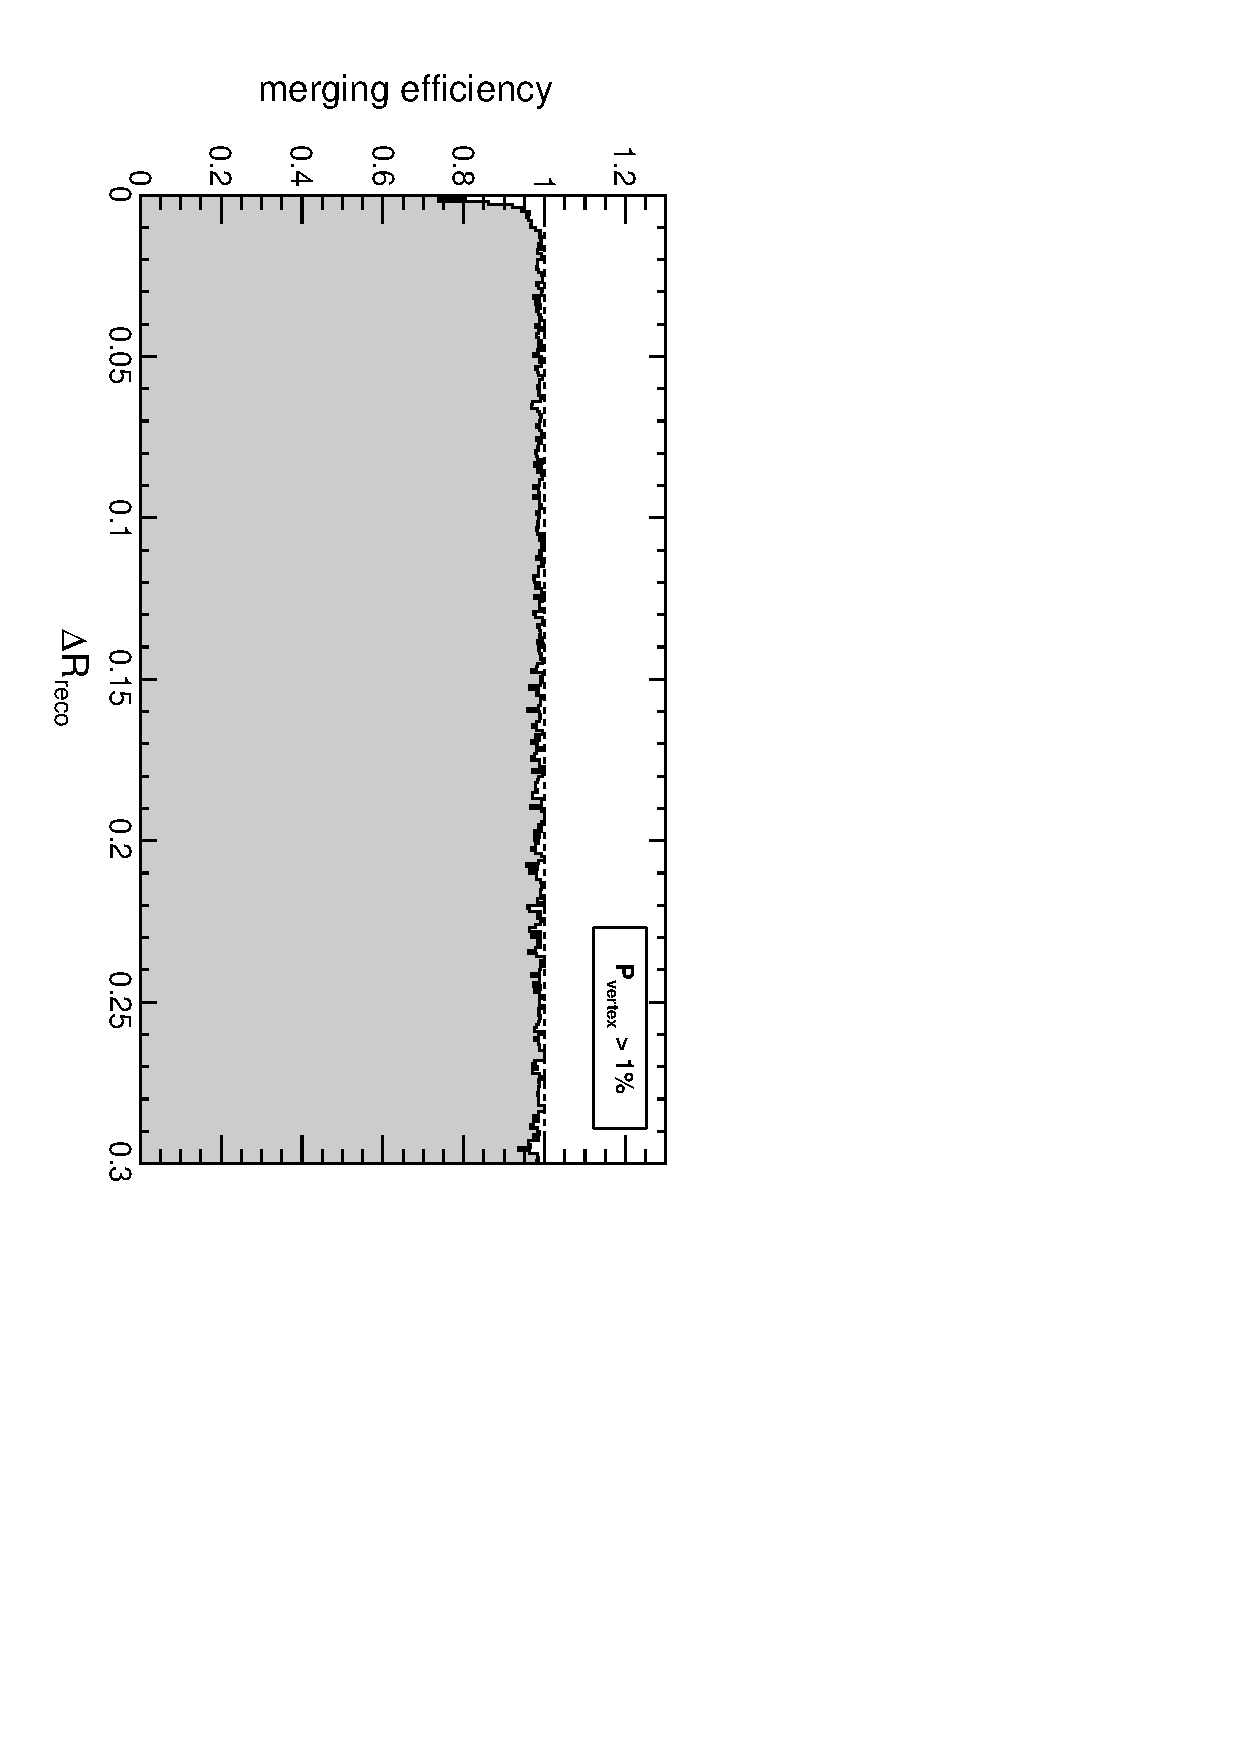
\includegraphics[height=0.5\linewidth, angle=90]{mergingeff_recodr_GroupByVertexProb.pdf}

\column{0.3\linewidth}
$\Delta R < 0.2$: finds muons that are geometrically close to each other

\vspace{0.25 cm}
$m_{\mbox{\scriptsize inv}} < 5$~GeV/$c$: finds low-mass objects, our physics goal

\vspace{0.25 cm}
$P_{\mbox{\scriptsize vertex}} > 1$\%: requires vertex compatibility (also physics goal); slightly inefficient when muons are nearly collinear

\end{columns}
\end{frame}

\begin{frame}
\frametitle{Supporting plots}

\begin{enumerate}
\item Cross-check: the vertex probability really does dip at very small masses
\item Quantitative comparison of $\Delta R$ and $m_{\mbox{\scriptsize inv}}$ (depends on sample's dimuon boost distribution, which goes up to $p_T = 100$~GeV/$c$)
\end{enumerate}

\vfill
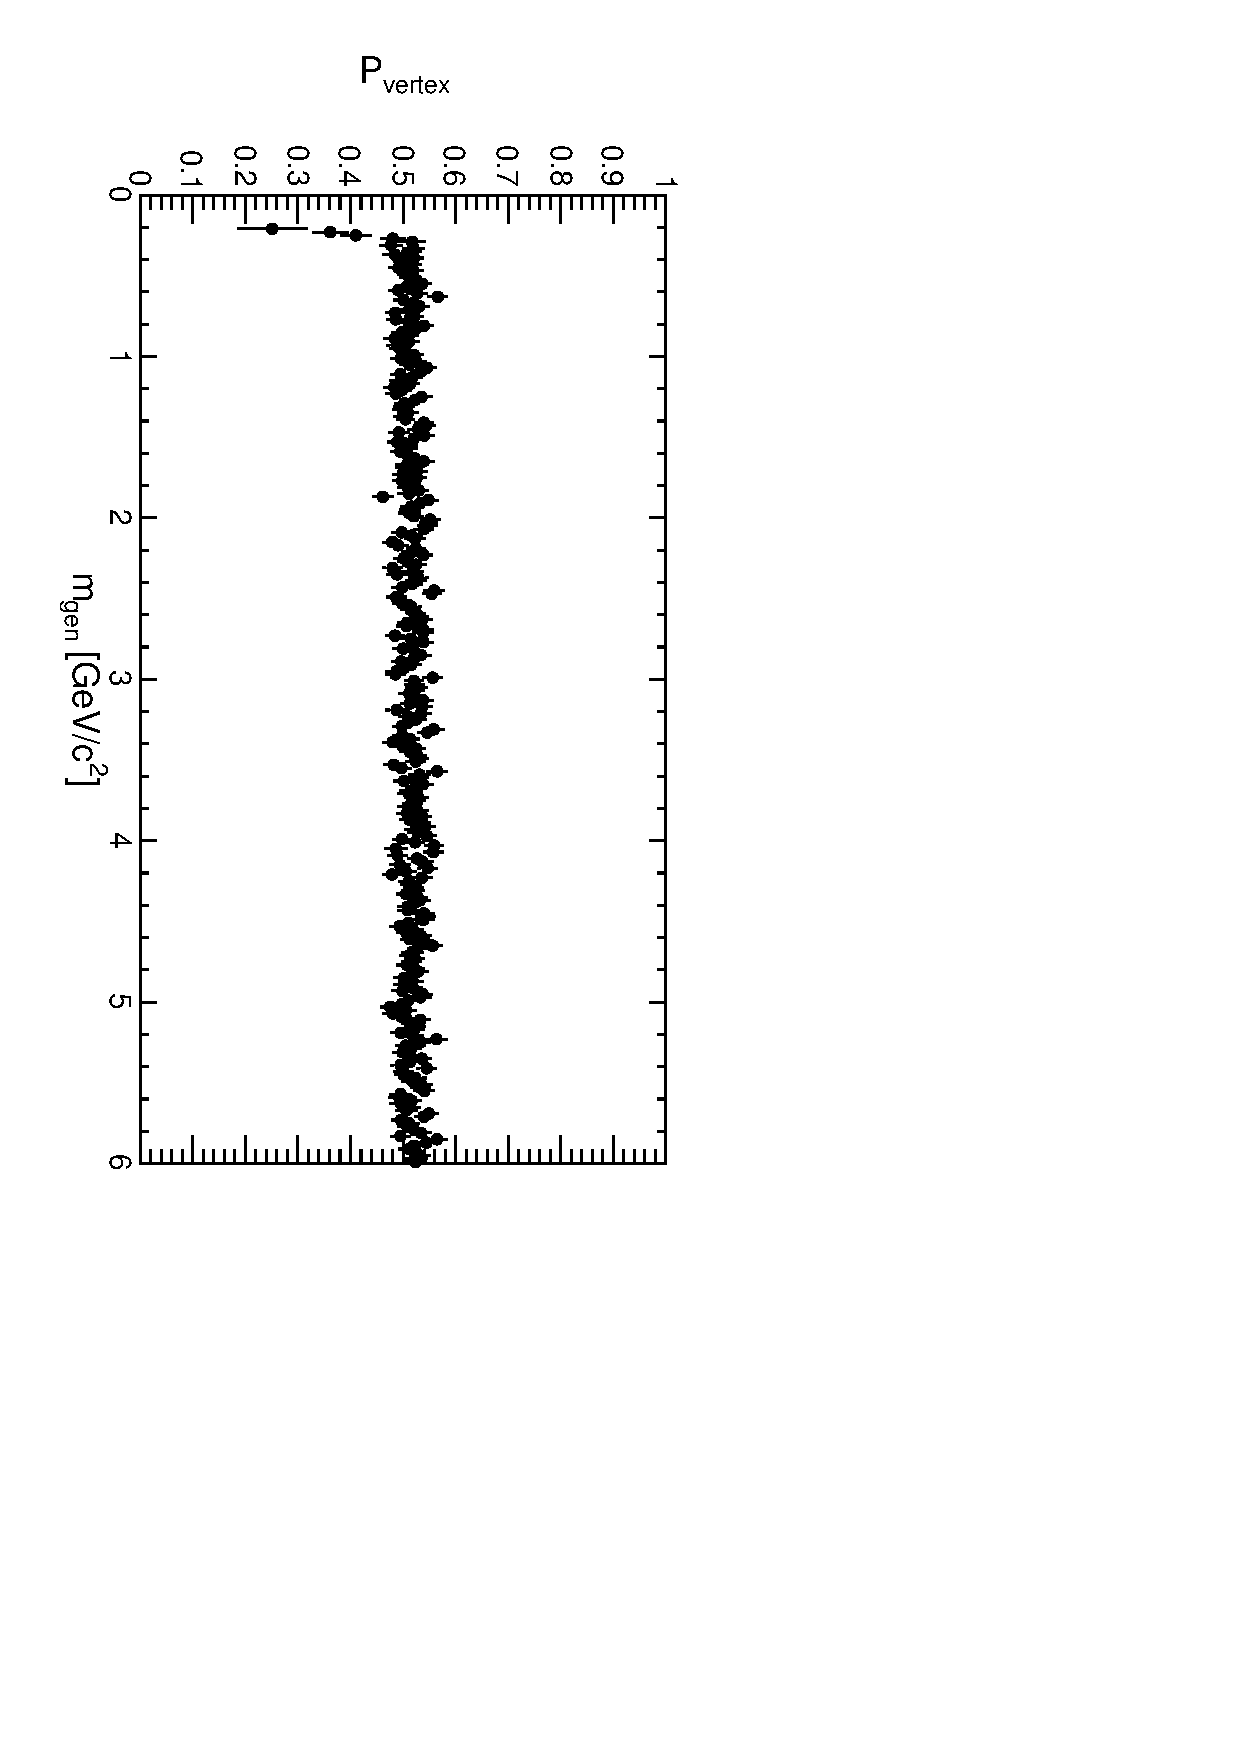
\includegraphics[height=0.5\linewidth, angle=90]{vertexProb_vs_mass.pdf}
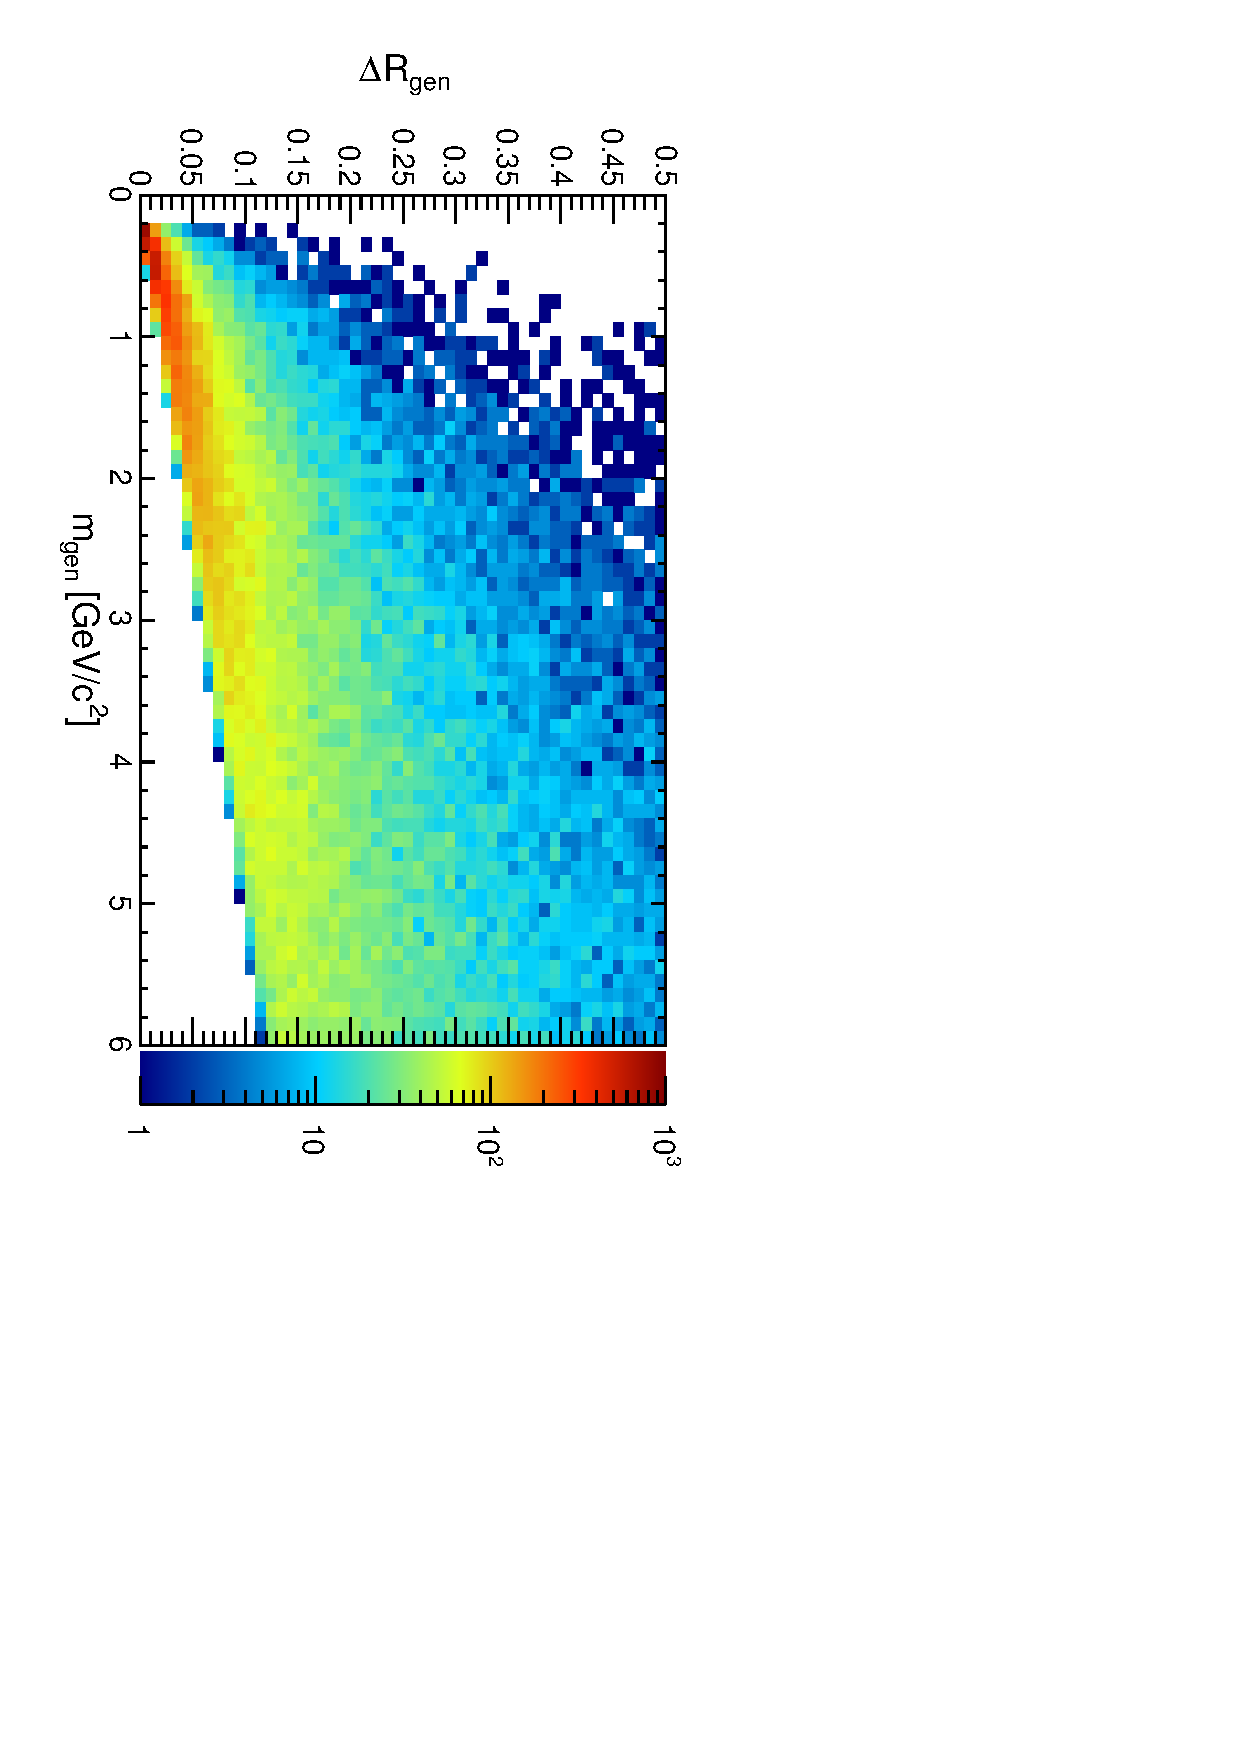
\includegraphics[height=0.5\linewidth, angle=90]{dr_vs_mass.pdf}
\end{frame}

\begin{frame}
\frametitle{Merging efficiency}
Best choice: group by $(m_{\mbox{\scriptsize inv}} < 5\mbox{ GeV/}c \mbox{\bf\mbox{ and }} P_{\mbox{\scriptsize vertex}} > 1\%) \mbox{\bf\mbox{ or }} \Delta R < 0.2$
\begin{itemize}
\item guarantees that we get the low-mass objects, for any boost (cut later on boost)
\item vertex probability guarantees that they came from the same origin
\item $\Delta R$ gets the tiny-mass case (though may want to reduce to $\Delta R < 0.1$ or 0.05 or something)
\end{itemize}

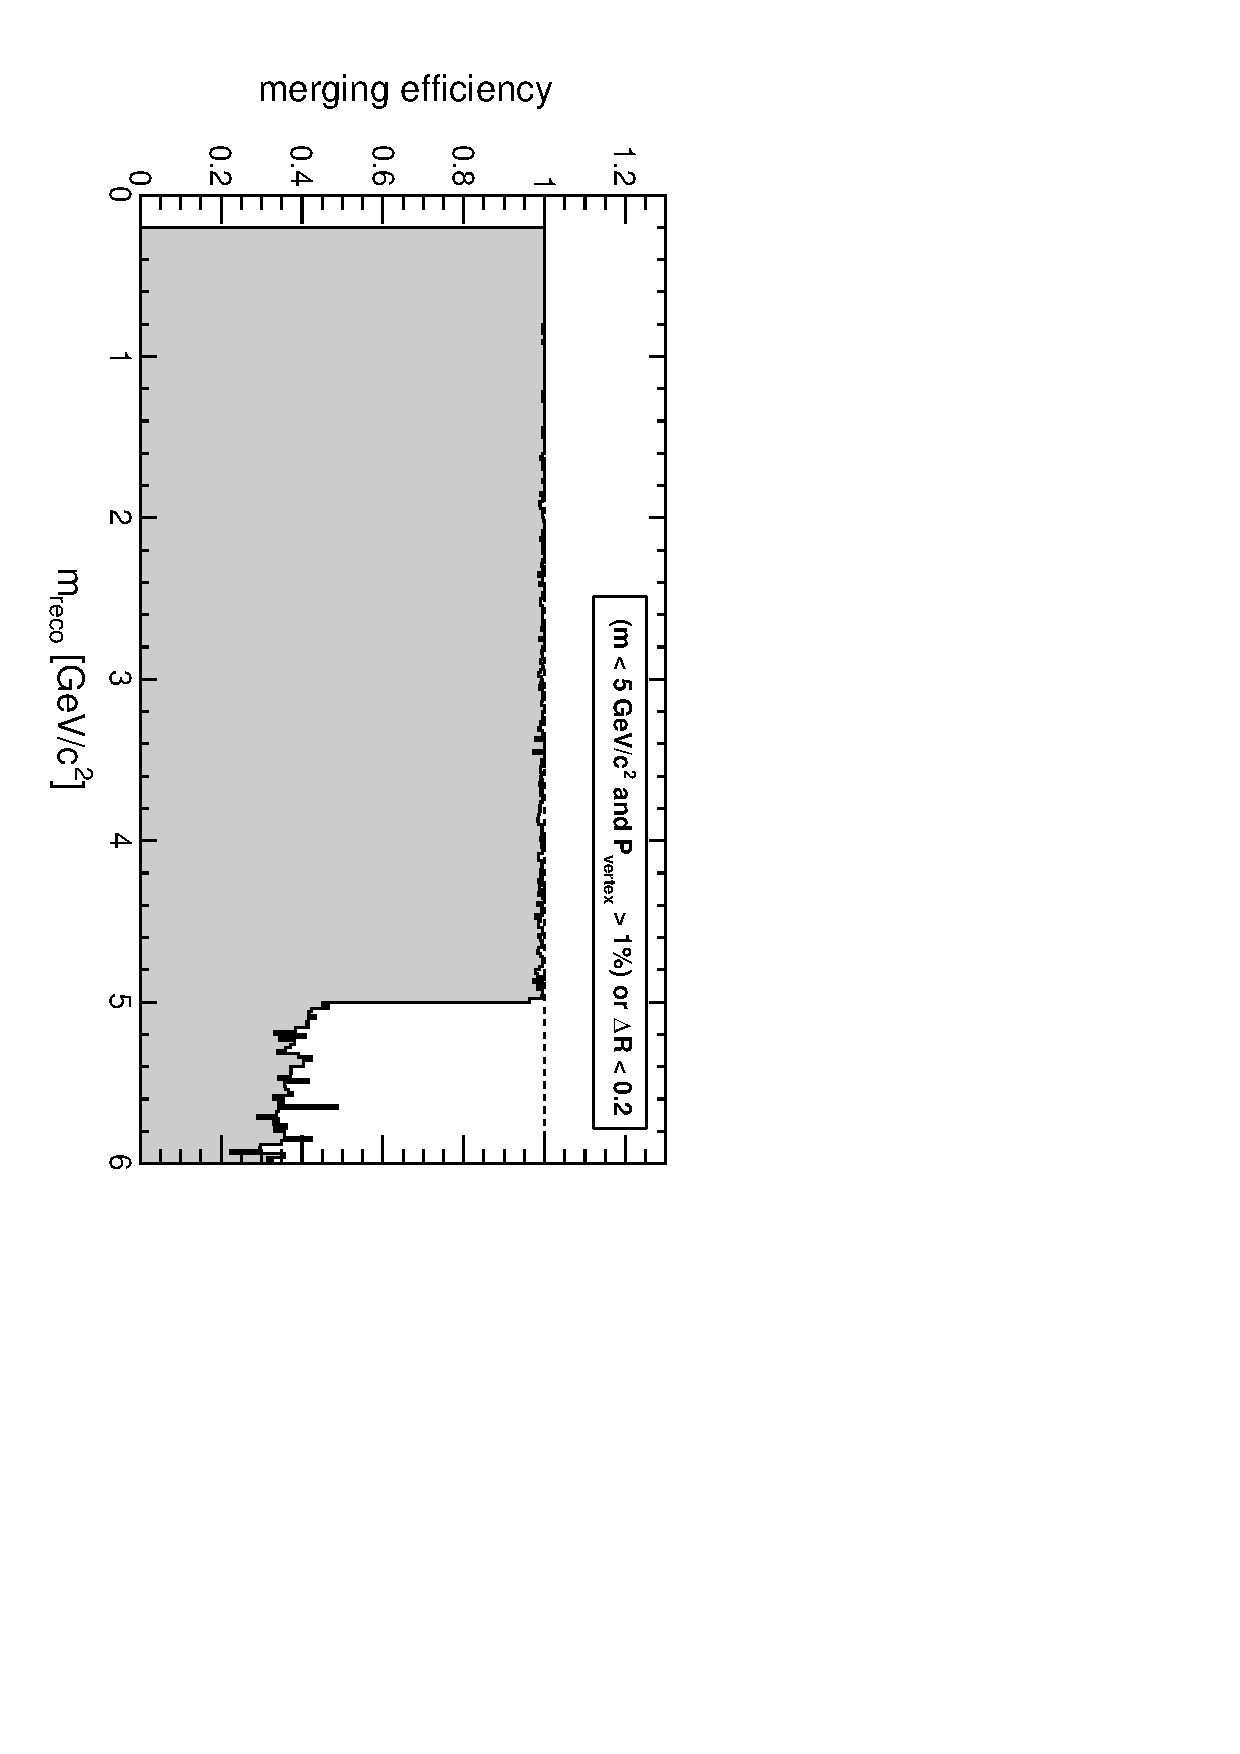
\includegraphics[height=0.5\linewidth, angle=90]{mergingeff_recomass_GroupByMassAndVertexProbOrDeltaR.pdf}
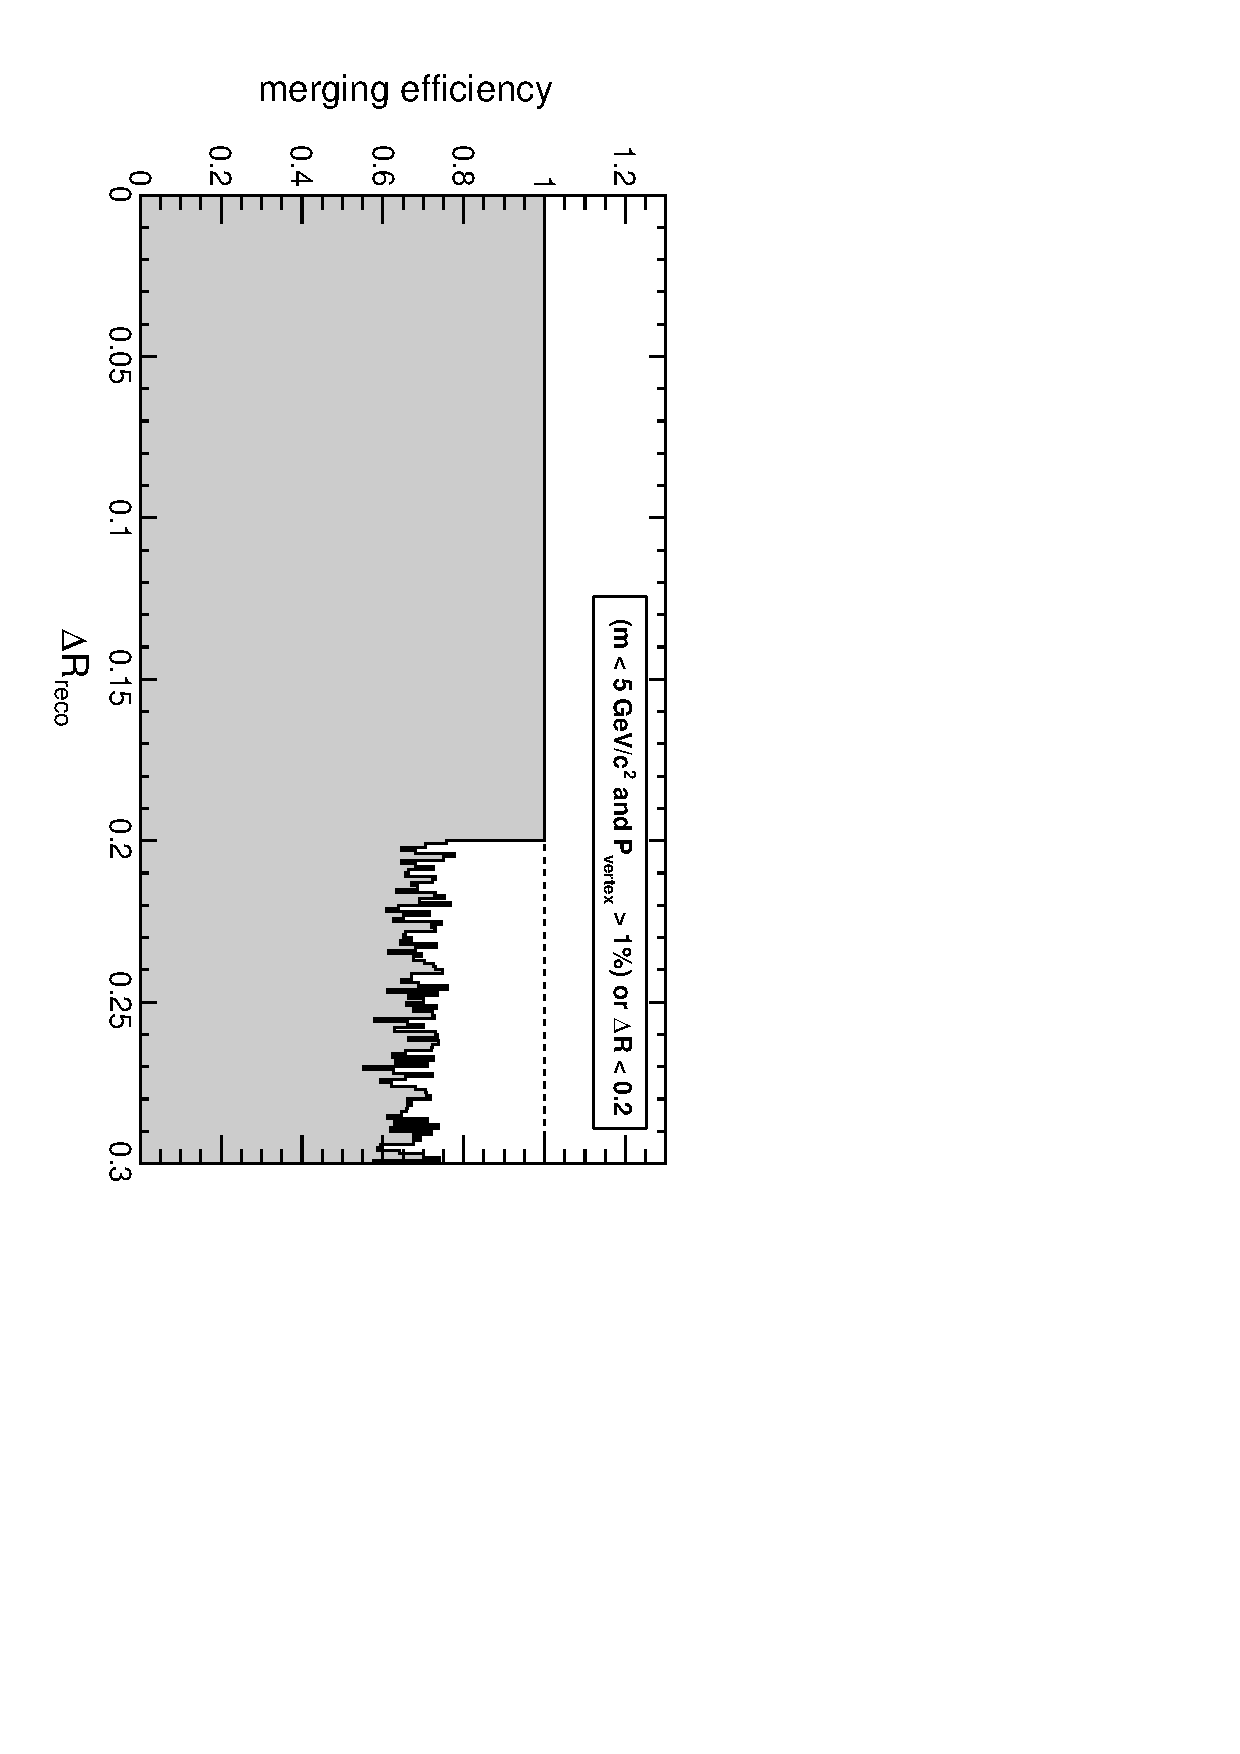
\includegraphics[height=0.5\linewidth, angle=90]{mergingeff_recodr_GroupByMassAndVertexProbOrDeltaR.pdf}
\end{frame}

\begin{frame}
\frametitle{Summary of efficiency}
These are TrackerMuons, plotted against the variable that we care about most

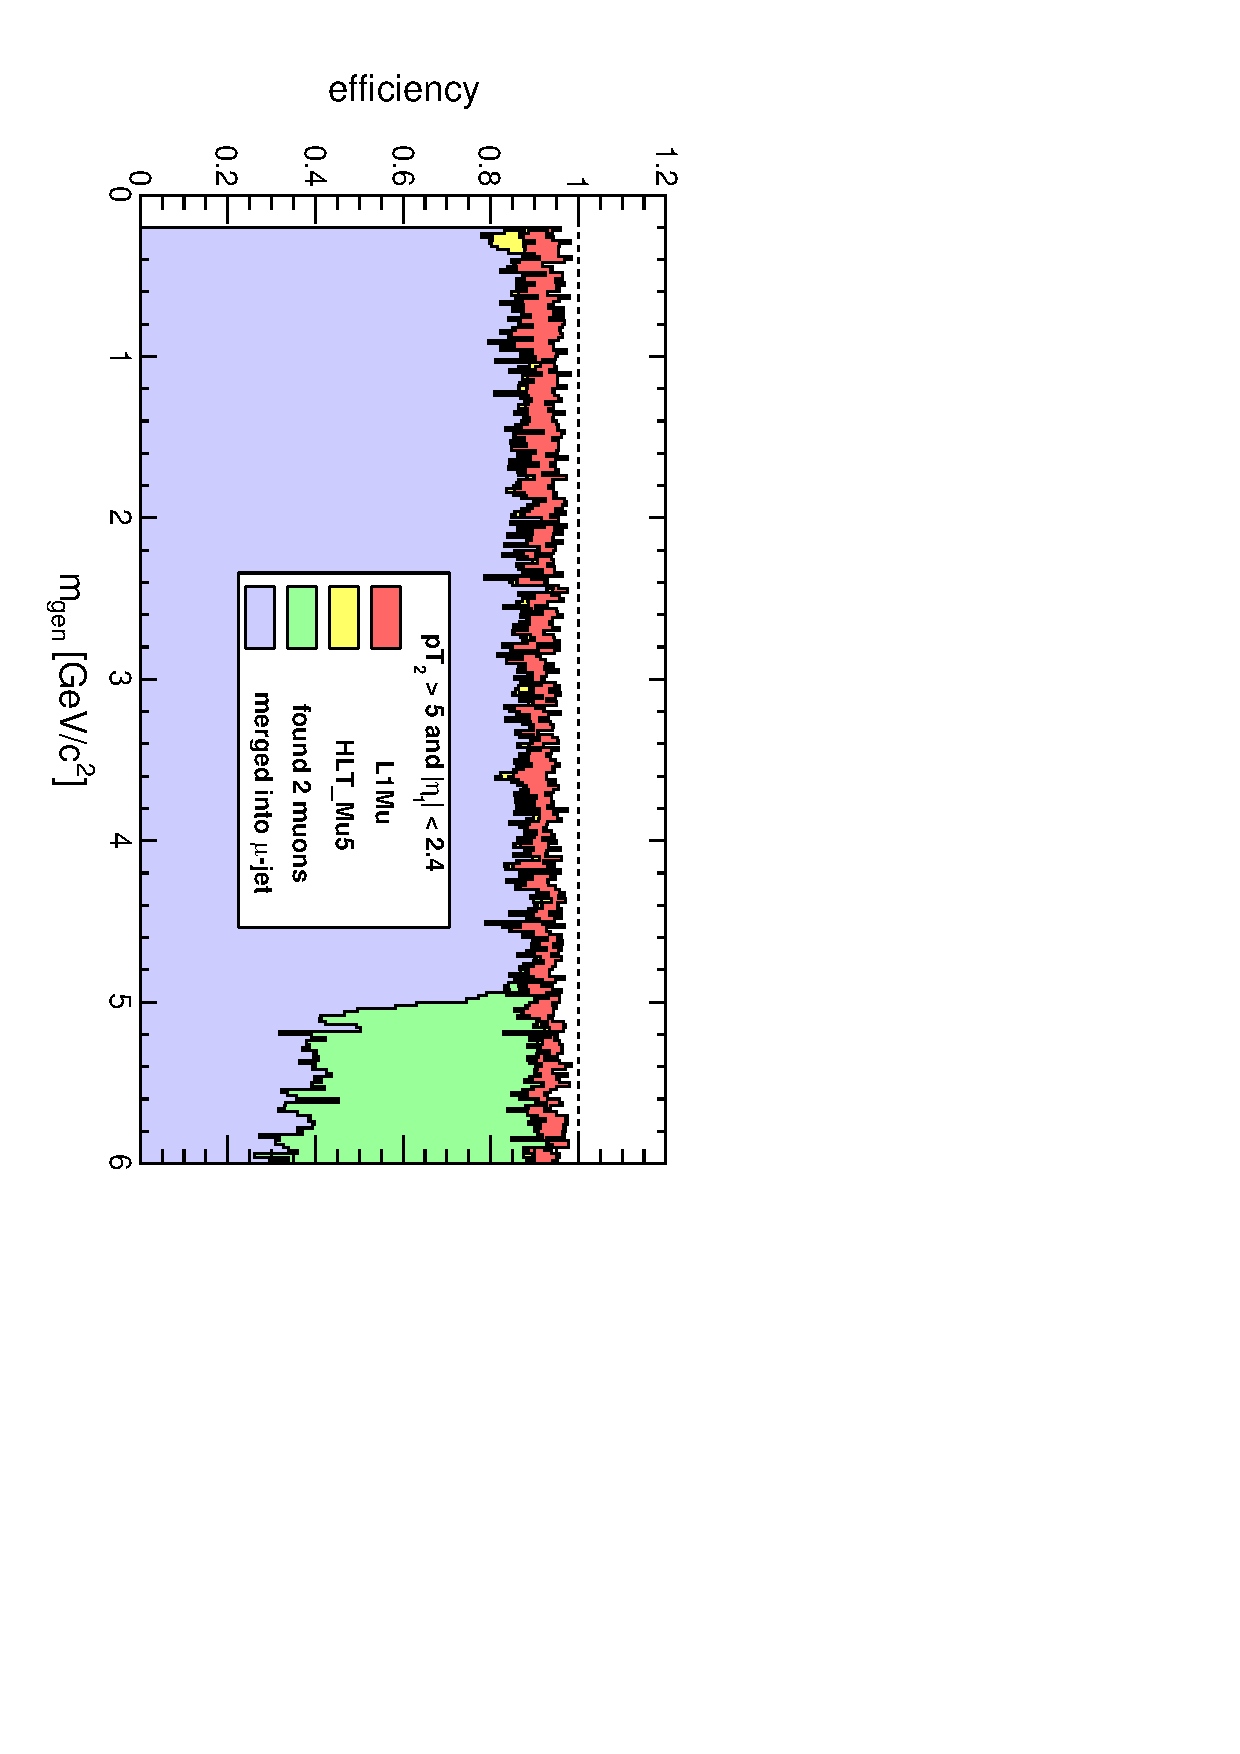
\includegraphics[height=\linewidth, angle=90]{mass.pdf}
\end{frame}

\begin{frame}
\frametitle{$\mu$-jet merging}

\begin{itemize}
\item In a new sample with two dimuons per event, how often do we find
  the two $\mu$-jets separately?
\begin{itemize}
\item ``two dimuons'' and ``one quadmuon'' are both discovery modes
\item $\Delta m_{\mbox{\scriptsize inv}}$ criteria in two searches can
  be tuned to make sure we overlap the whole discovery region
\end{itemize}
\item $\alpha_{\mbox{\scriptsize pair-pair}}$ is the opening angle between the two dimuon axes
\item ``Crossed'' $\mu$-jets are when you get two pairs but with the wrong association (1-3, 2-4 instead of 1-2, 3-4)
\item Varying the merging criteria changes this plot as you'd expect
\end{itemize}

\only<1>{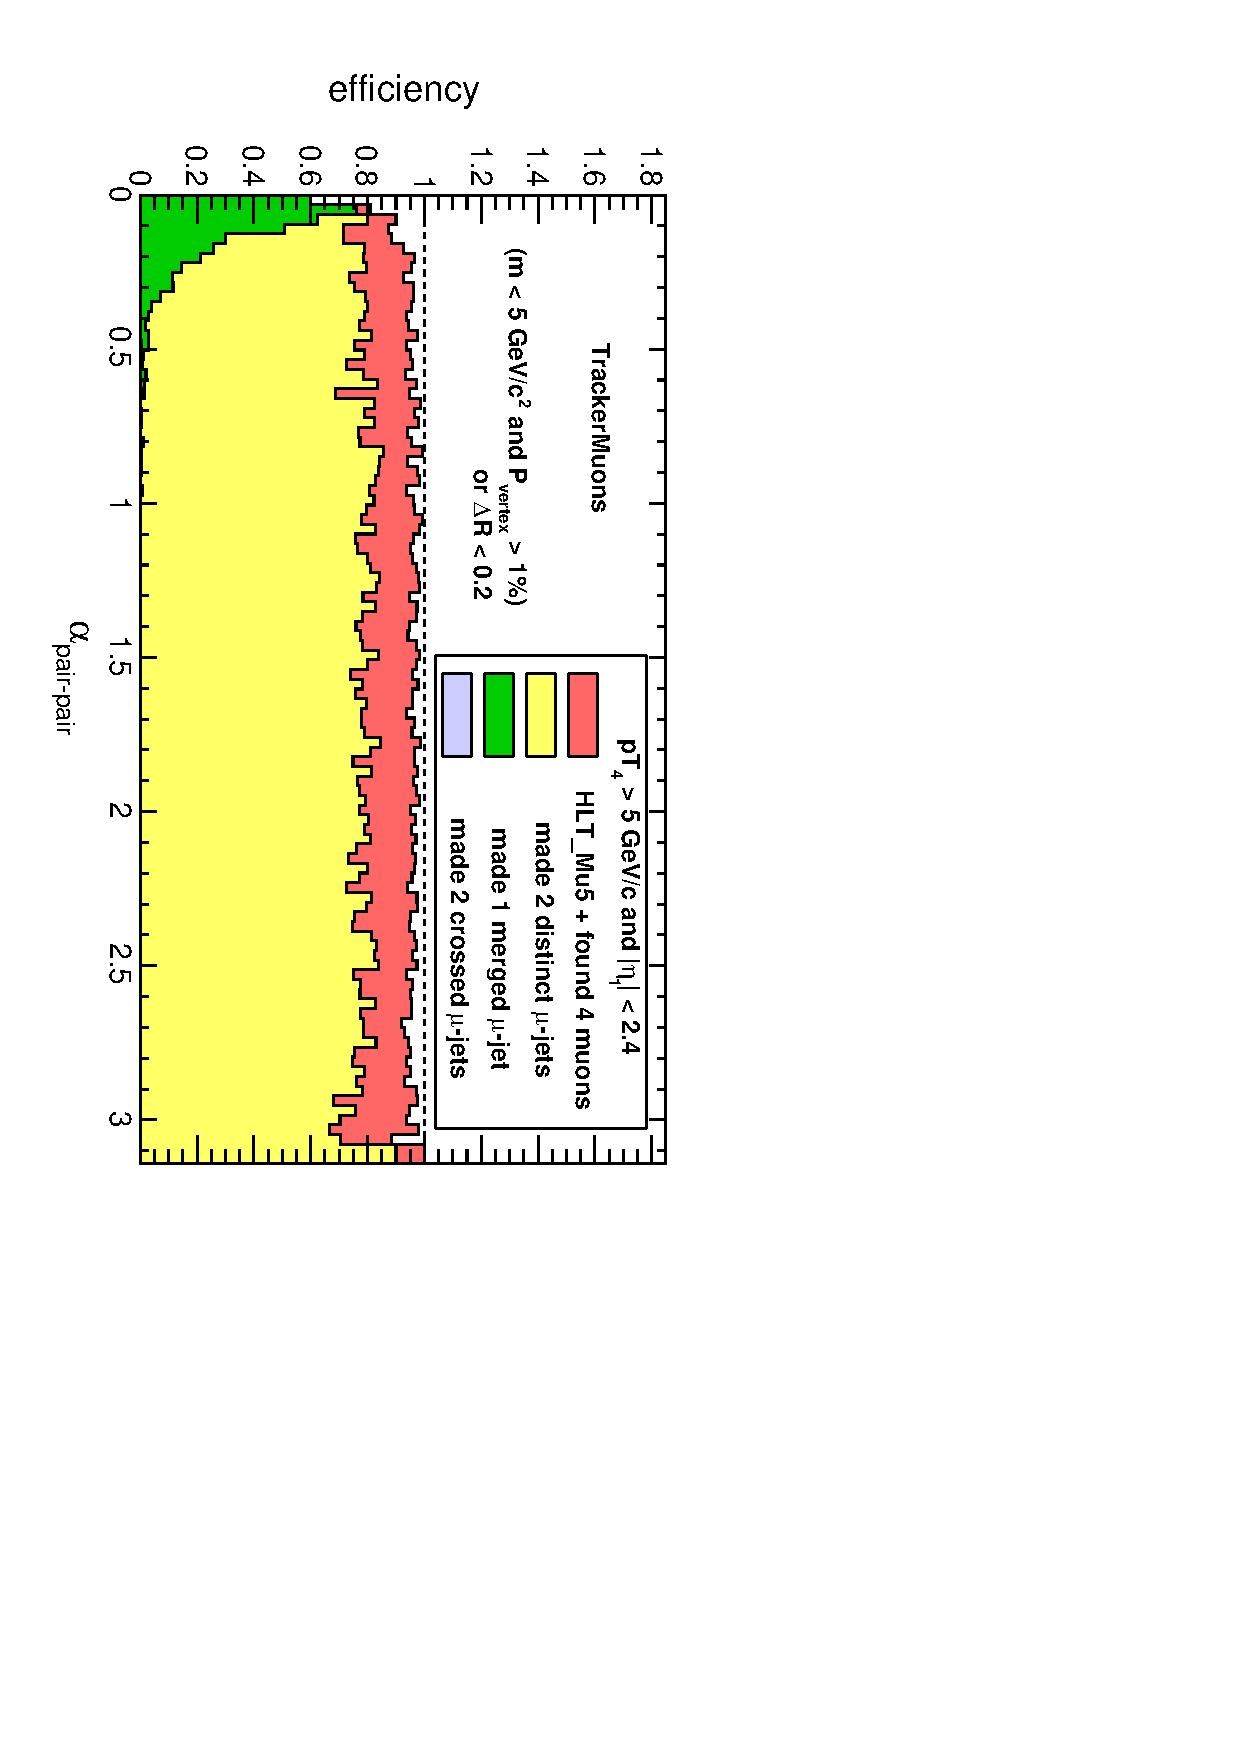
\includegraphics[height=0.5\linewidth, angle=90]{foundopening_TrackerMuonsGroupByMassAndVertexProbOrDeltaR.pdf}
  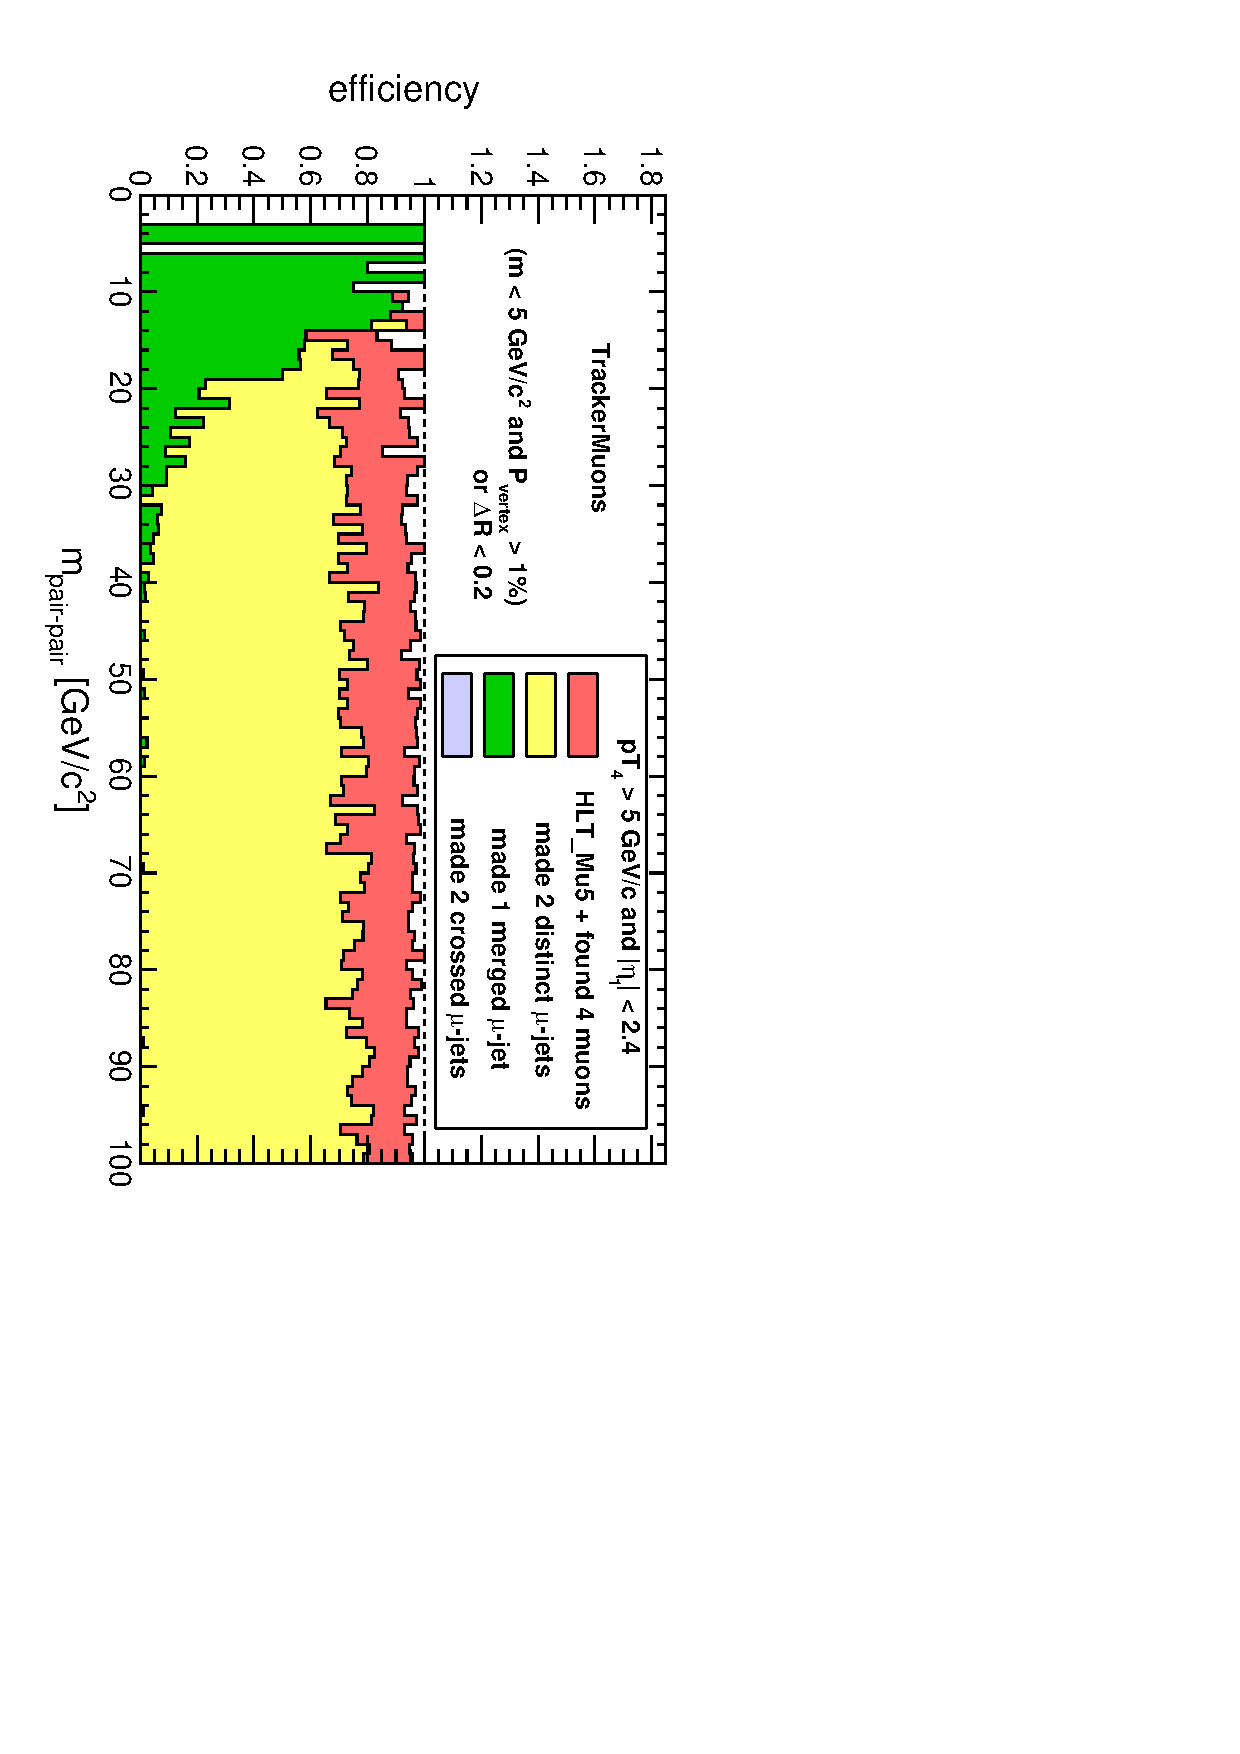
\includegraphics[height=0.5\linewidth, angle=90]{foundmass_TrackerMuonsGroupByMassAndVertexProbOrDeltaR.pdf}}
\only<2>{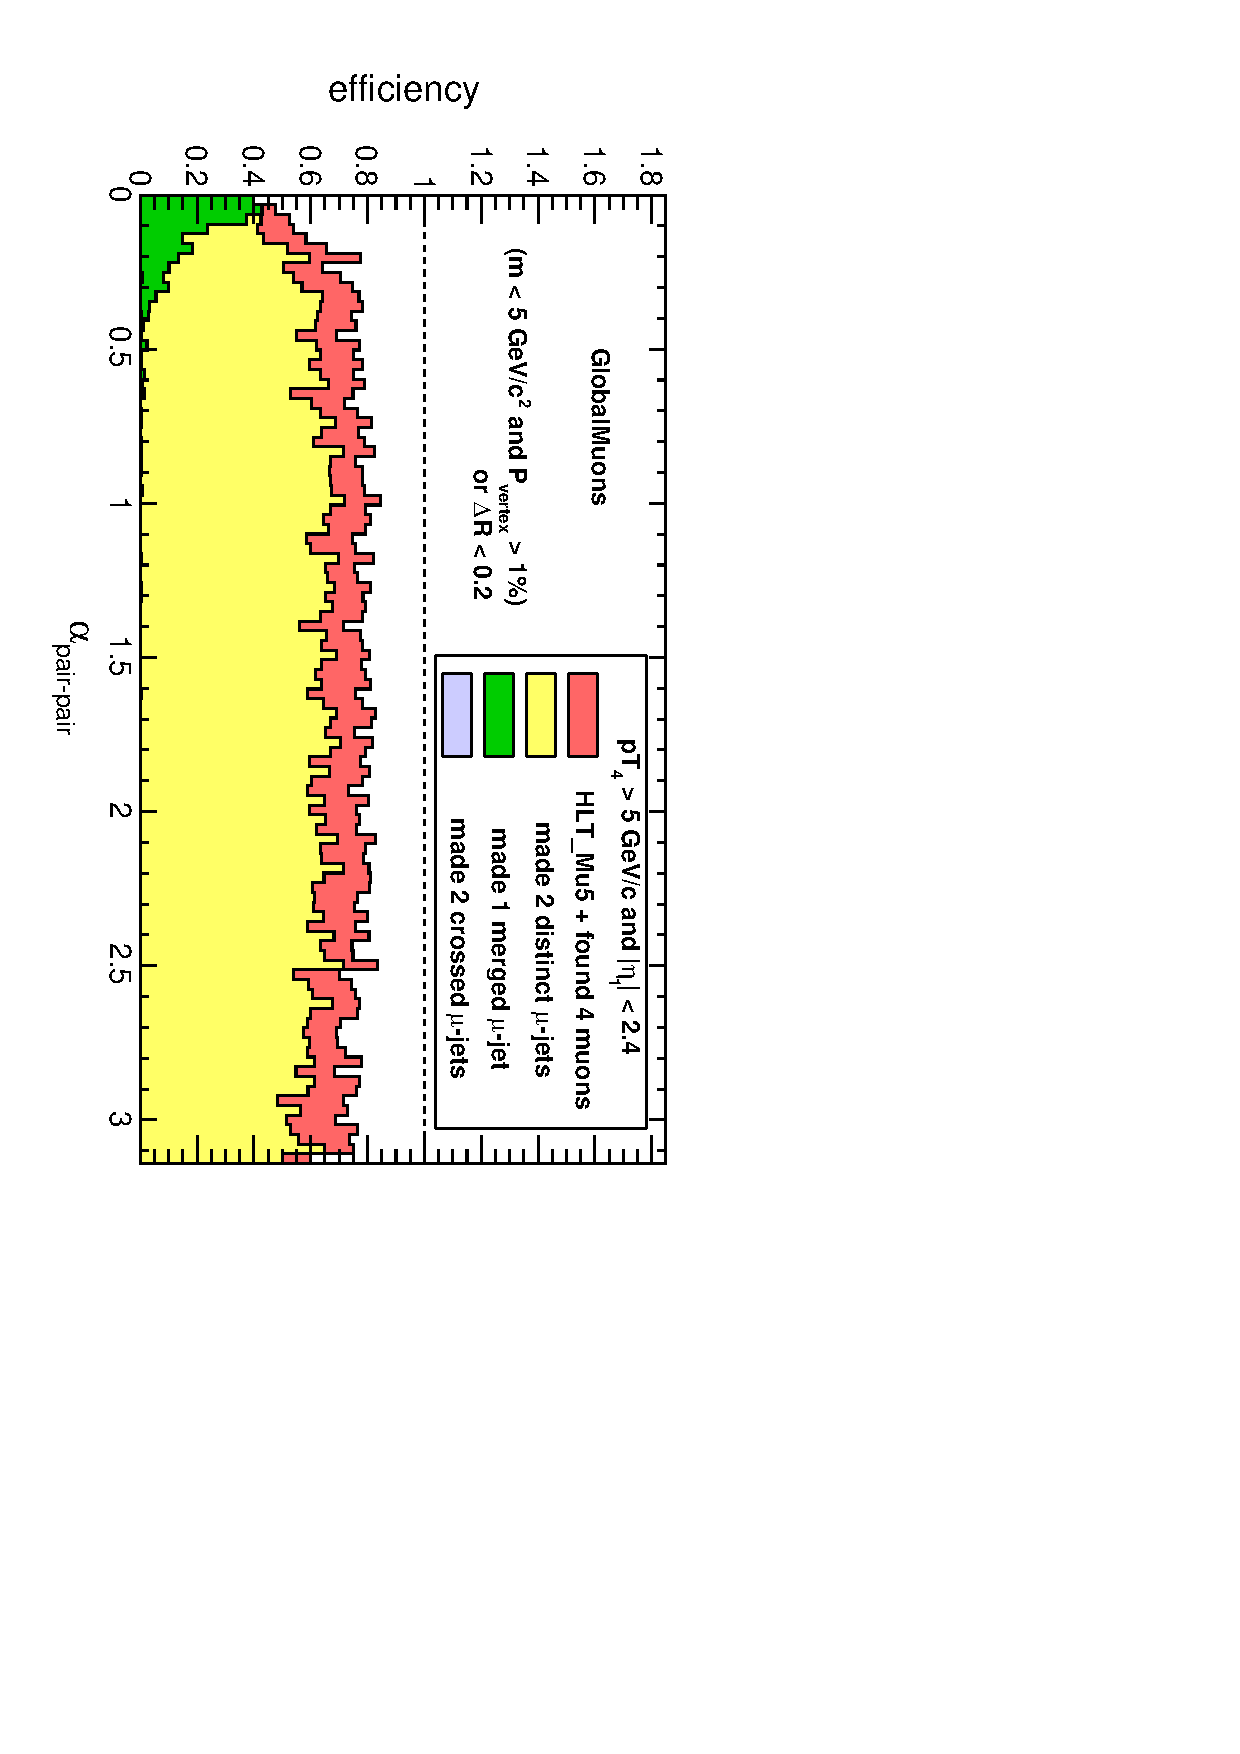
\includegraphics[height=0.5\linewidth, angle=90]{foundopening_GlobalMuonsGroupByMassAndVertexProbOrDeltaR.pdf}
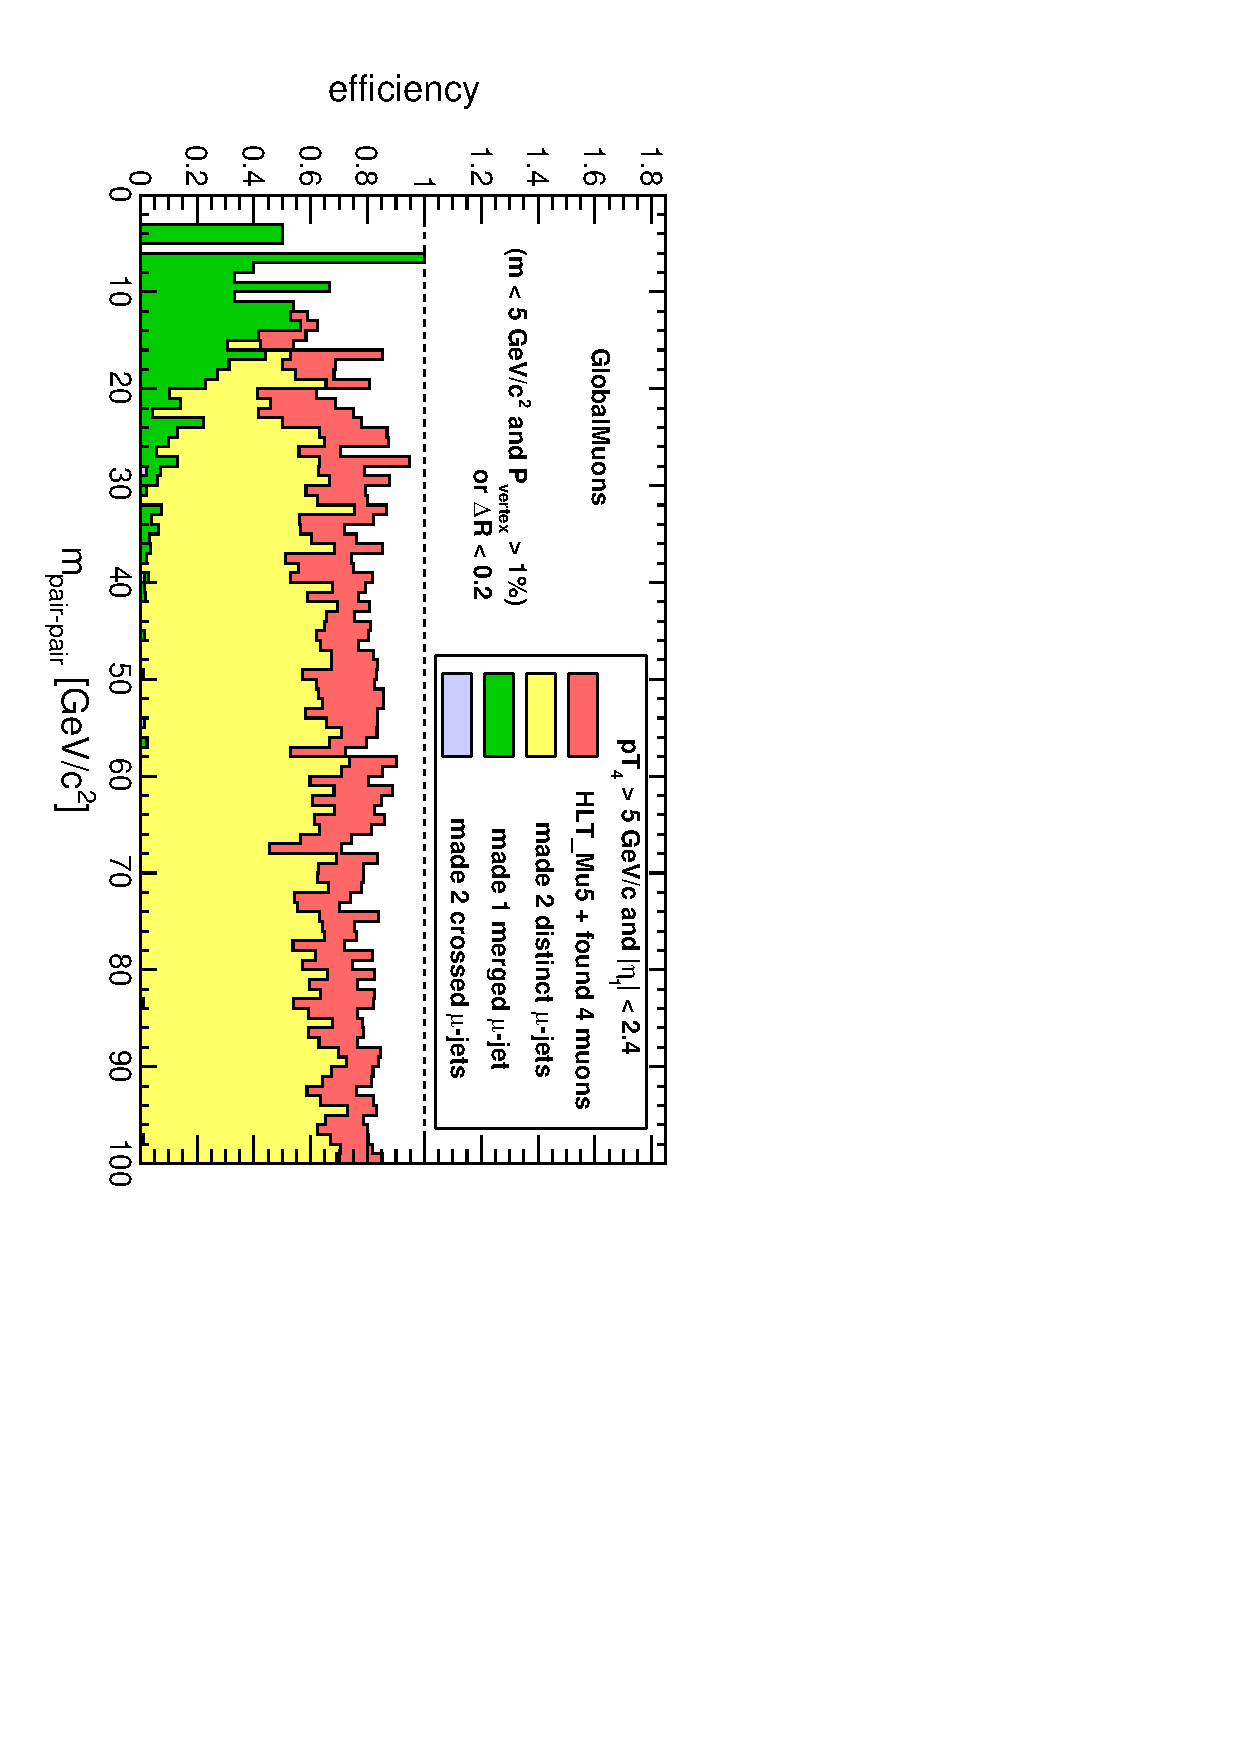
\includegraphics[height=0.5\linewidth, angle=90]{foundmass_GlobalMuonsGroupByMassAndVertexProbOrDeltaR.pdf}}
\end{frame}

\begin{frame}
\frametitle{4-muon reconstruction efficiency}

\begin{itemize}
\item This depends on $pT_4$ vs.\ $\eta_1$ (remember our paper?)
\item Until I see the backgrounds, I would apply $pT_4 > 5$~GeV/$c$ and $\eta_1 < 2.4$

(Our paper additionally had $pT_1 > 20$~GeV/$c$; I'll check to see if it's really needed)

\item Also, I want to check the ``optimized arbitration'' I talked about last time to see if we can do the analysis with TrackerMuons, but that, too is a backgrounds study
\end{itemize}

\vfill
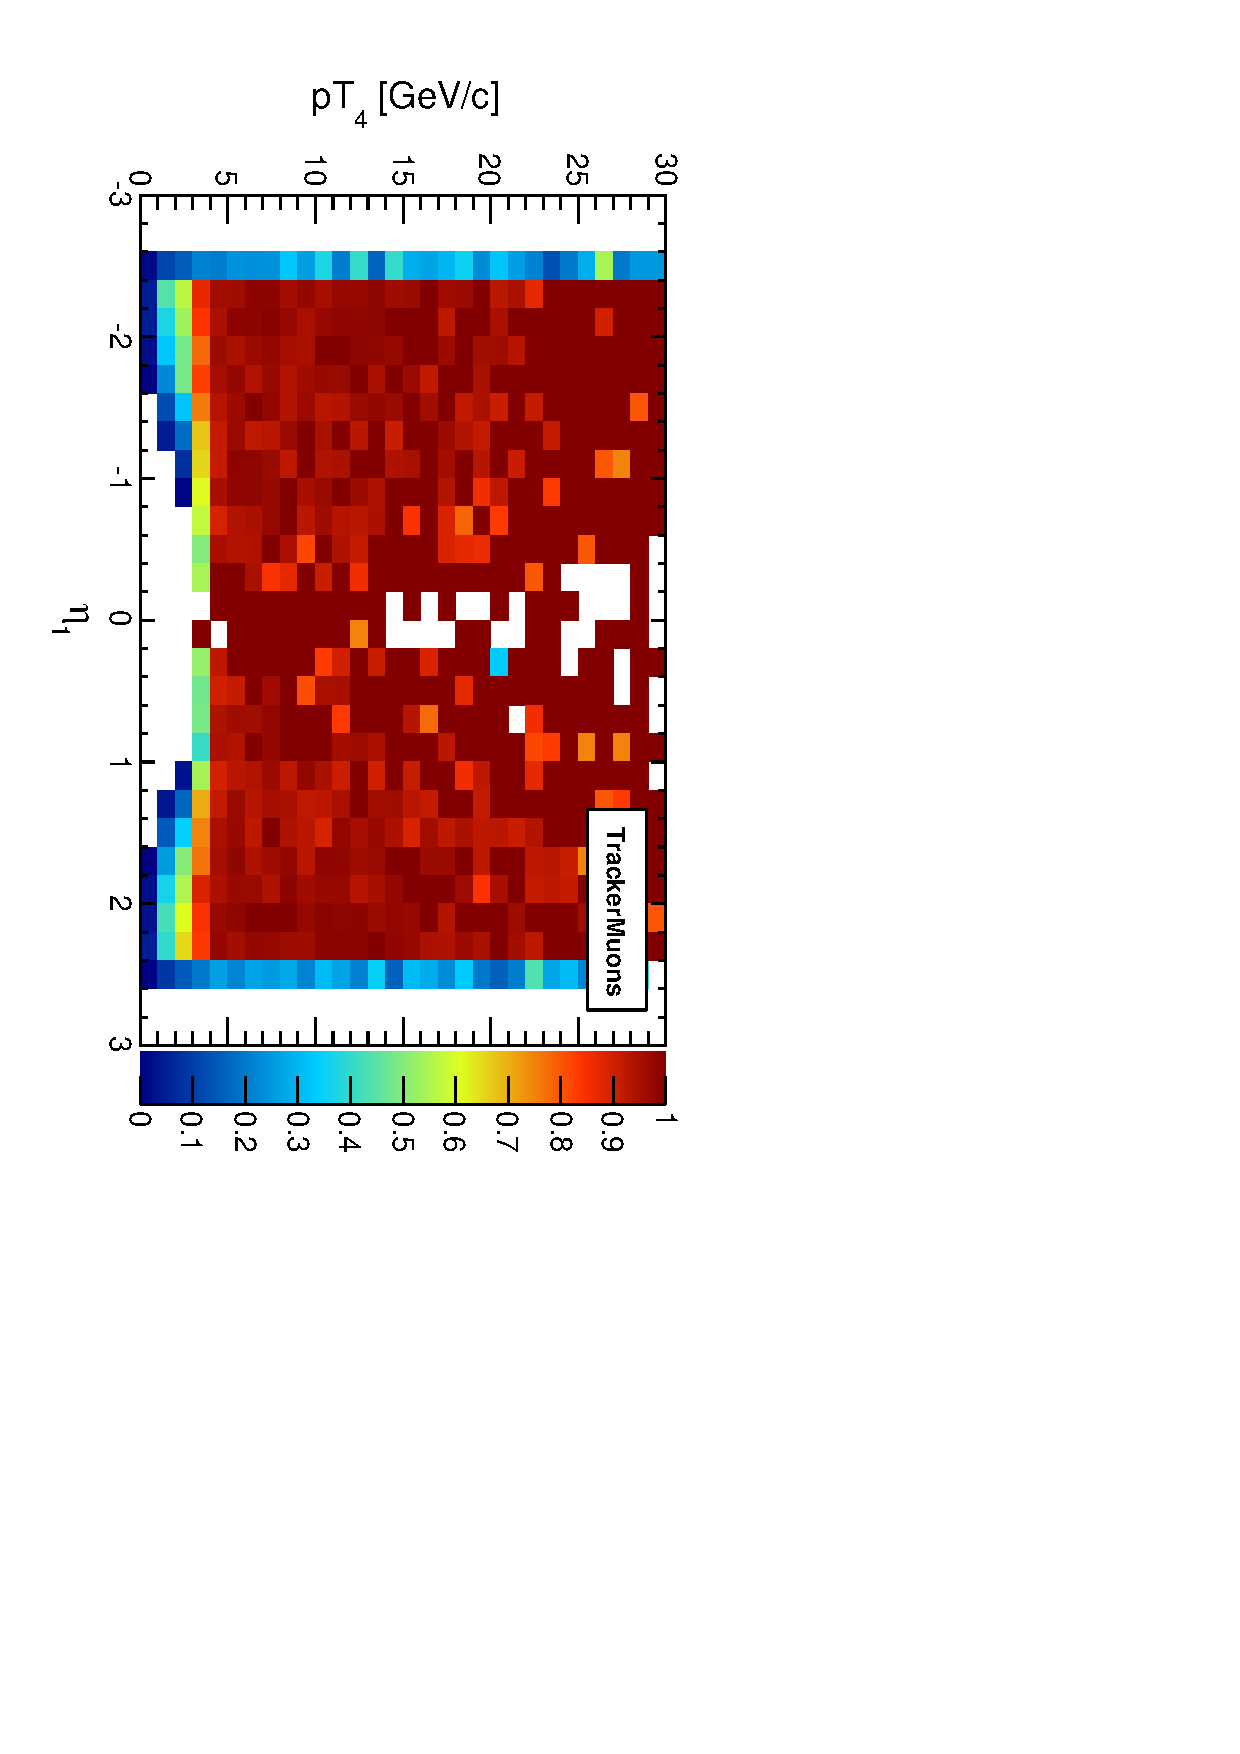
\includegraphics[height=0.5\linewidth, angle=90]{pt4vseta1_TrackerMuons.pdf}
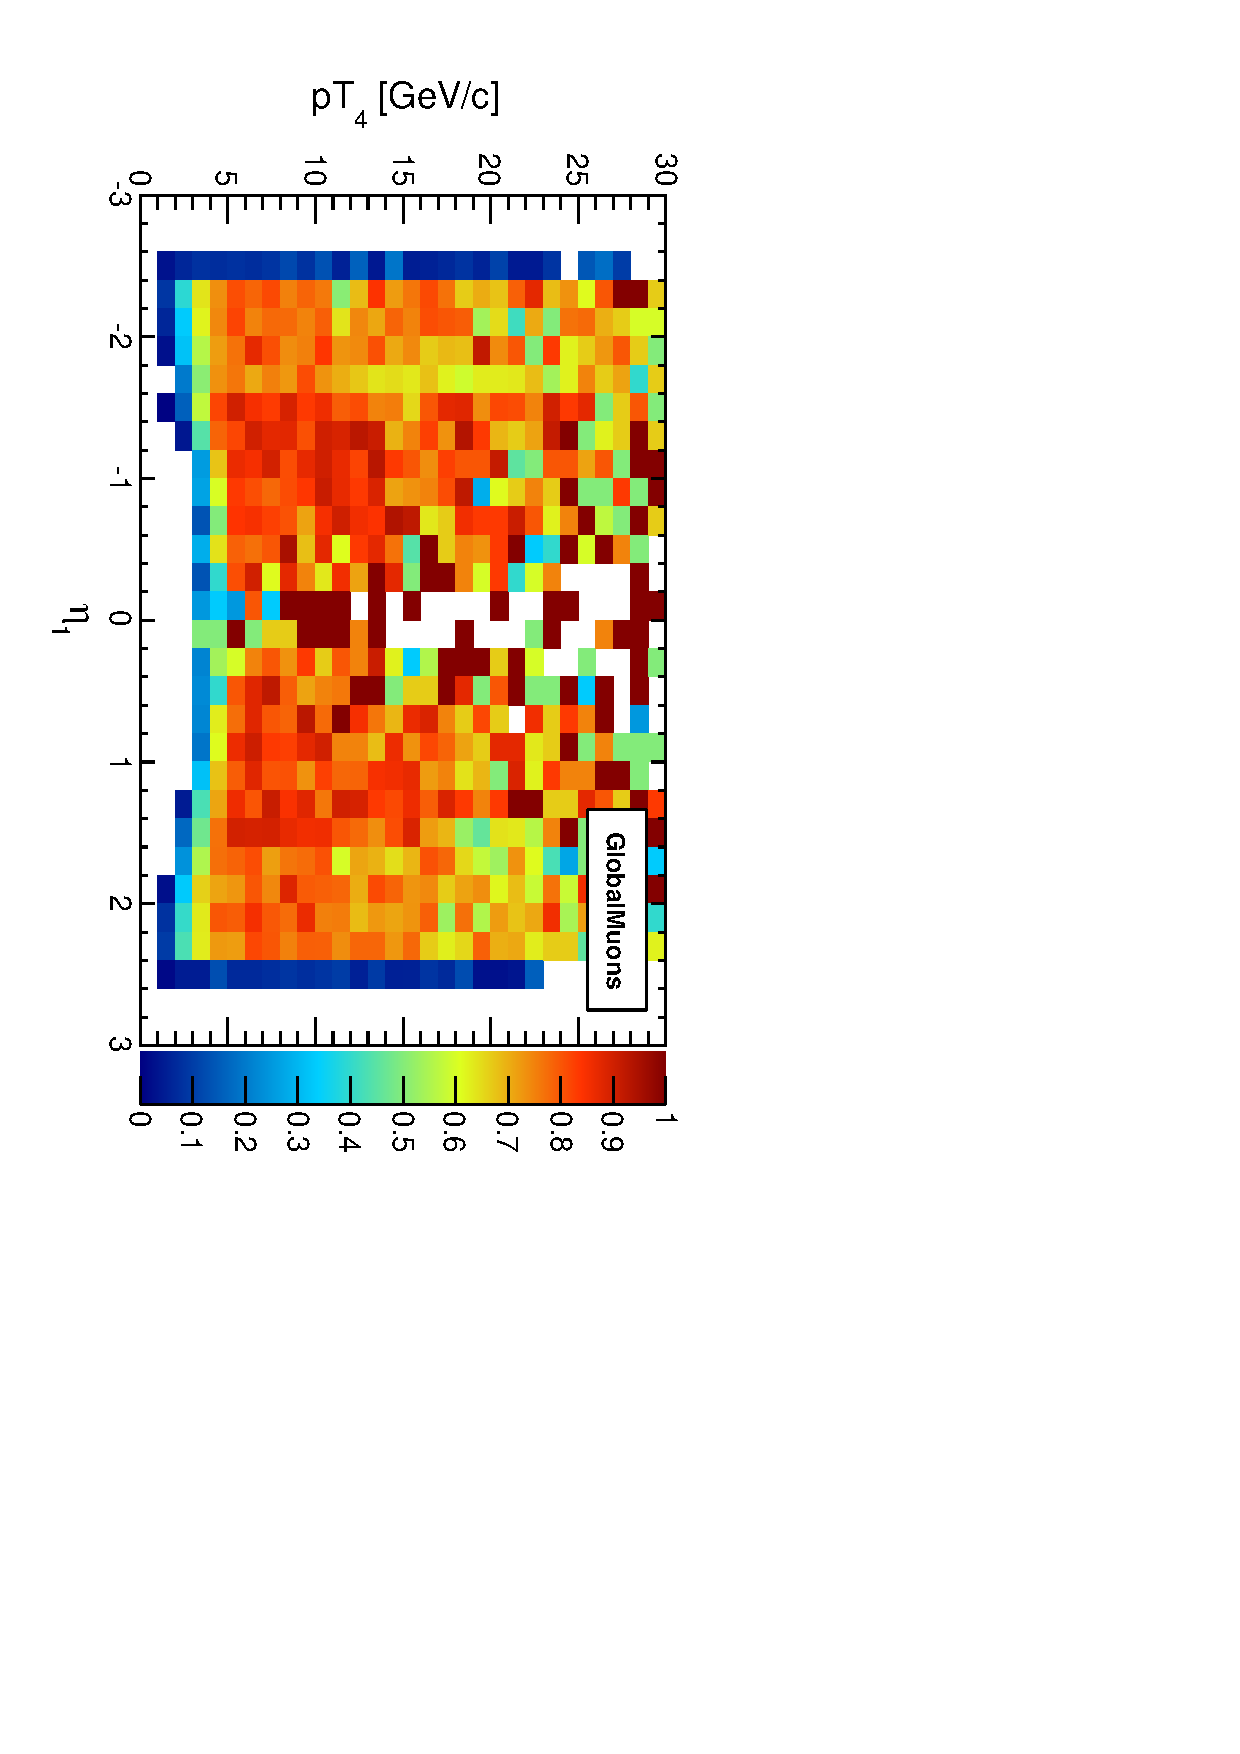
\includegraphics[height=0.5\linewidth, angle=90]{pt4vseta1_GlobalMuons.pdf}
\end{frame}

\begin{frame}
\frametitle{Pair-pair mass constraint}

Mostly interesting for supressing backgrounds, but here are the signal studies

\begin{columns}
\column{0.5\linewidth}
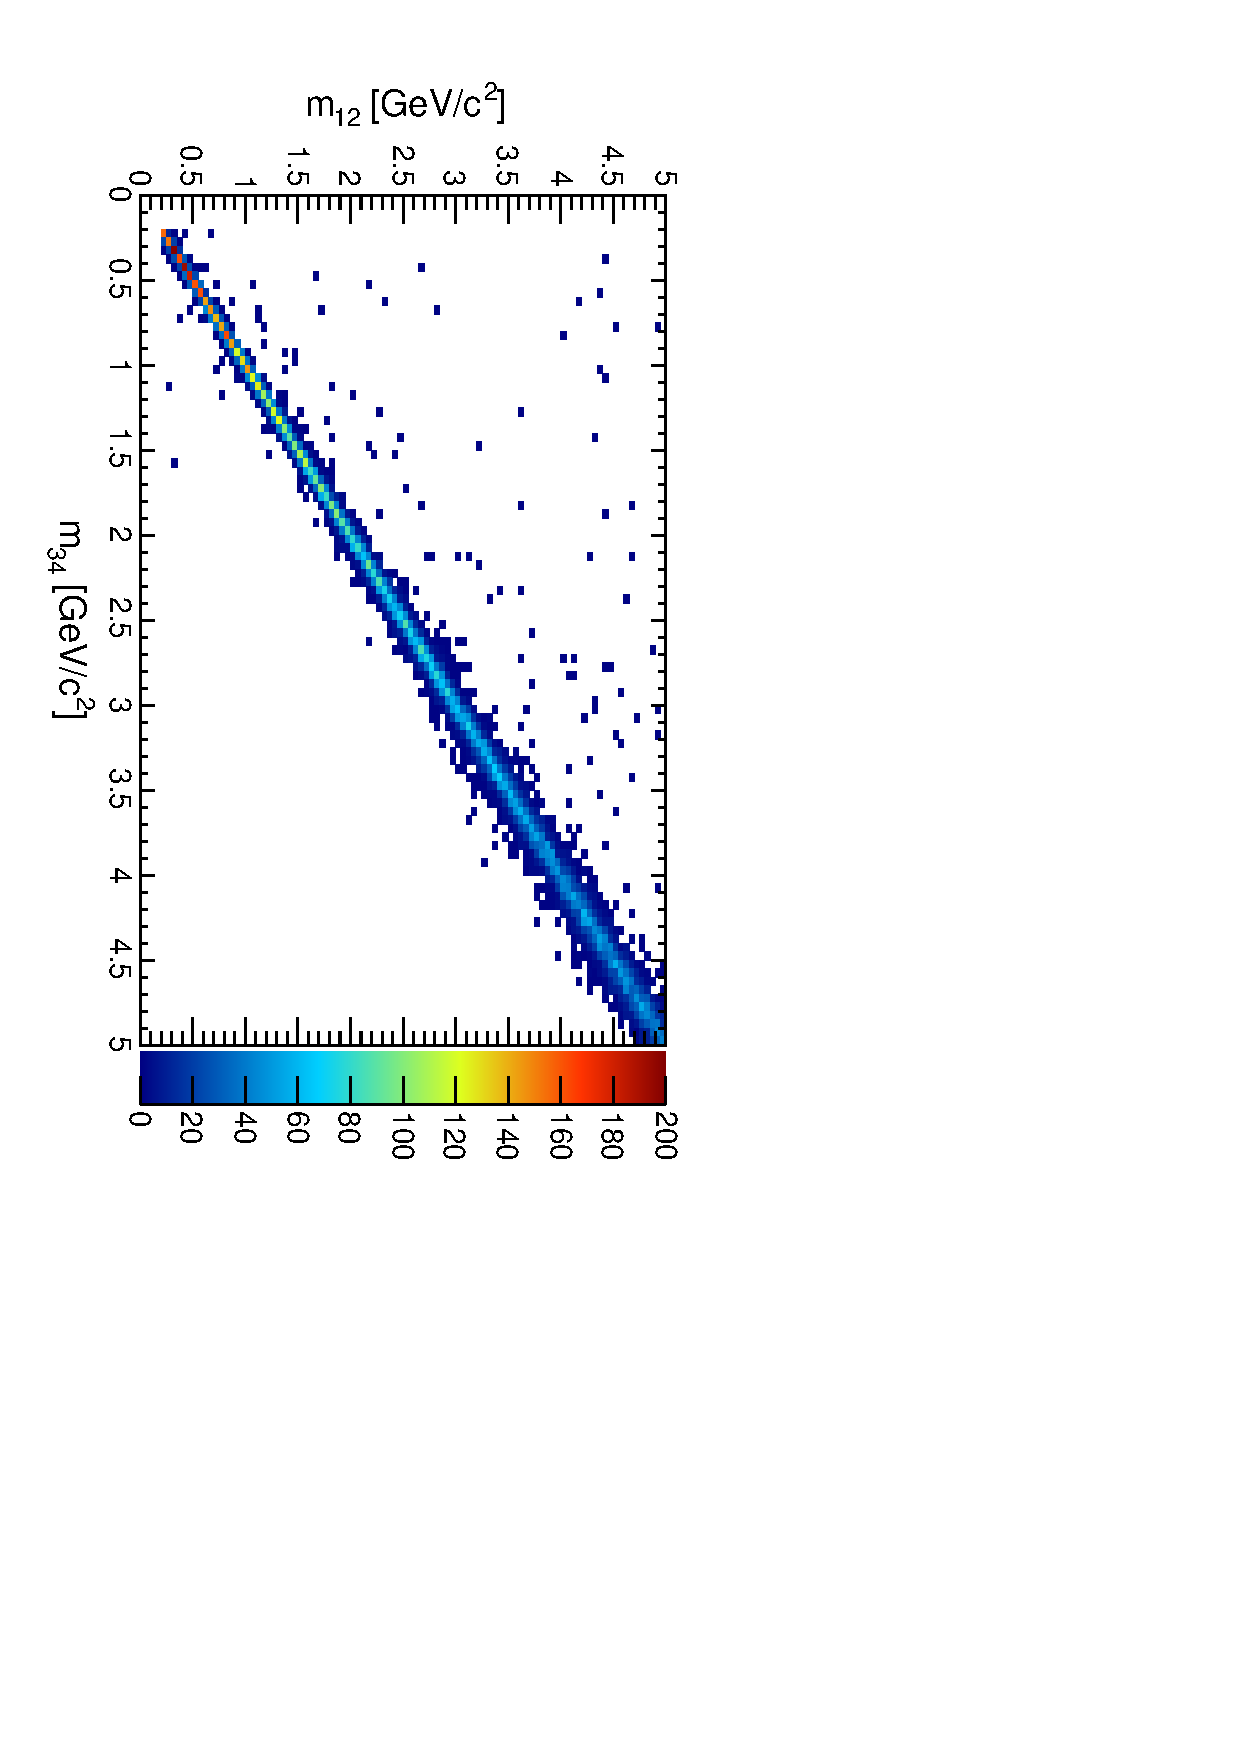
\includegraphics[height=\linewidth, angle=90]{m12m34.pdf}

\column{0.5\linewidth}
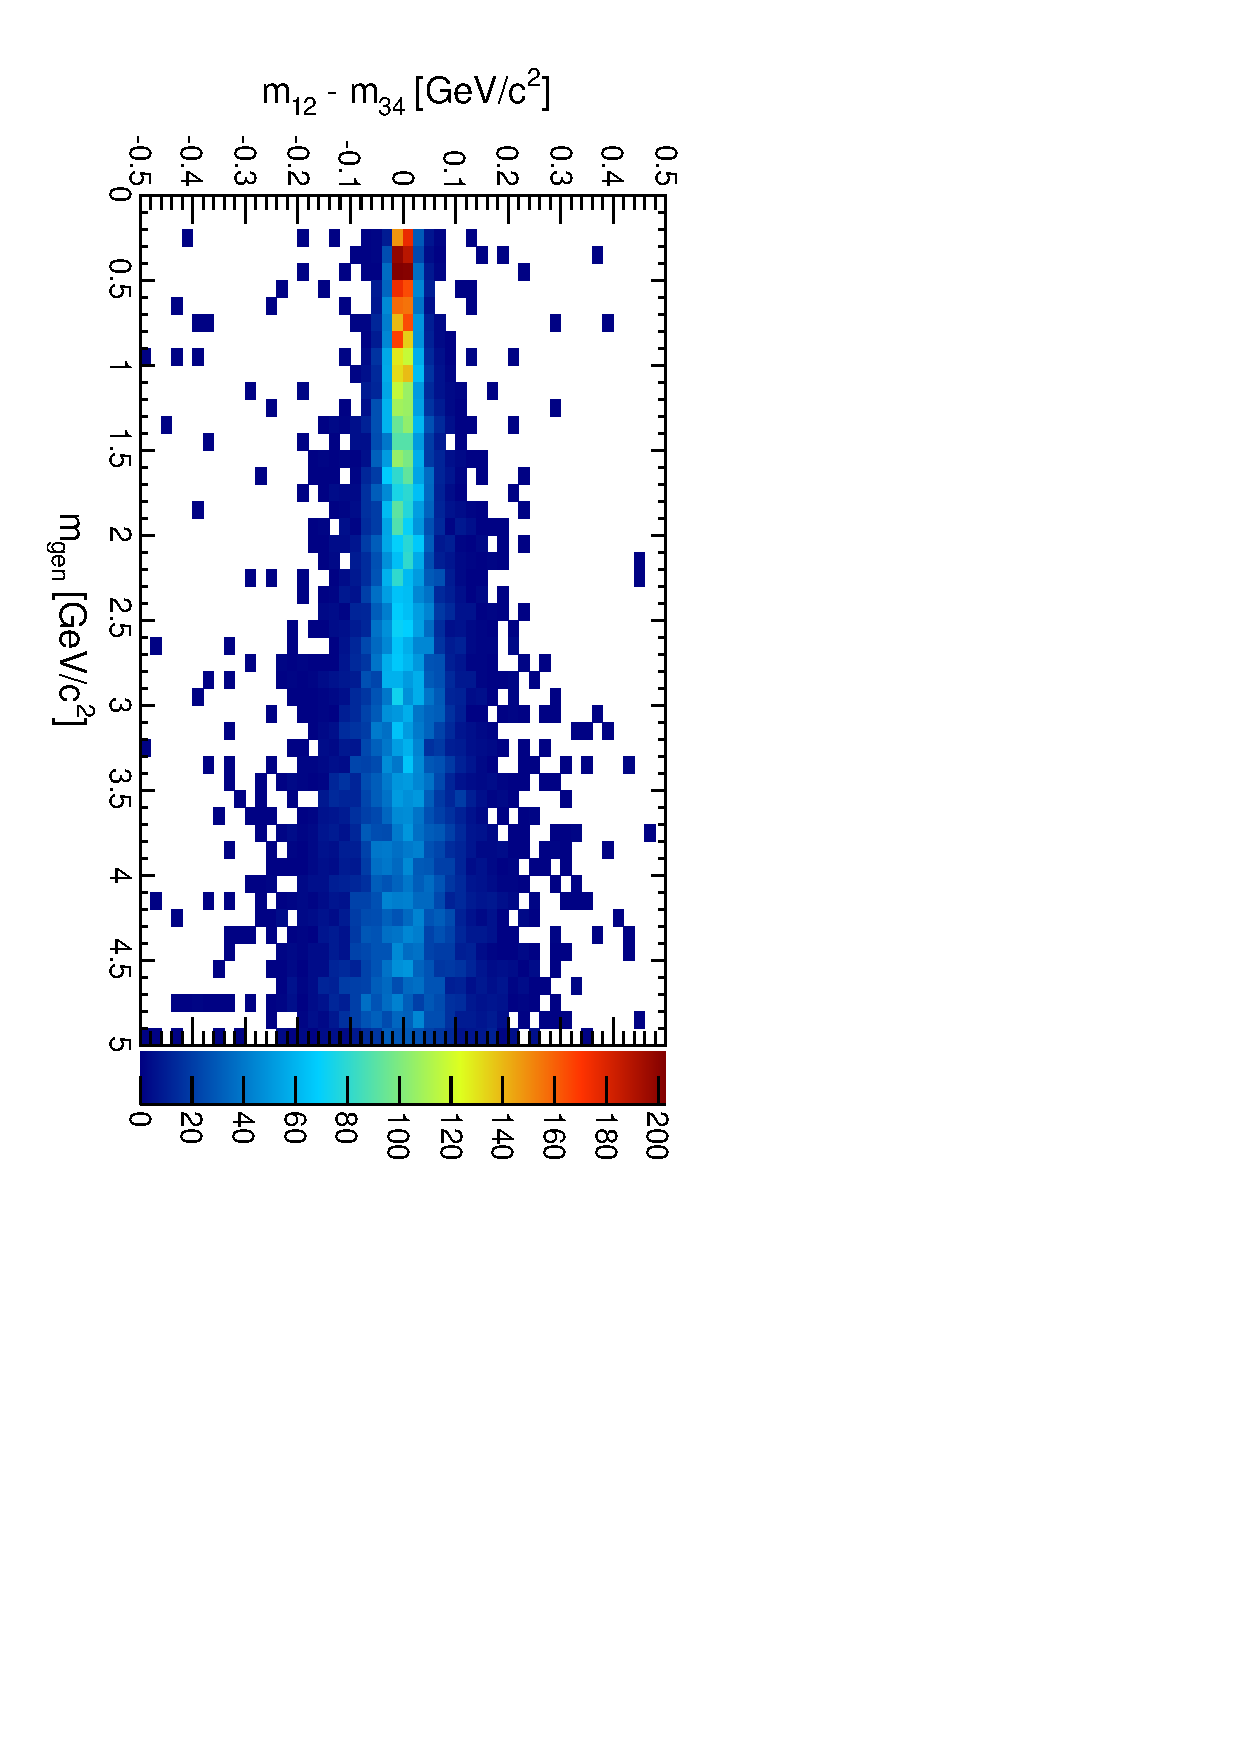
\includegraphics[height=\linewidth, angle=90]{mdiff_vs_mass.pdf}

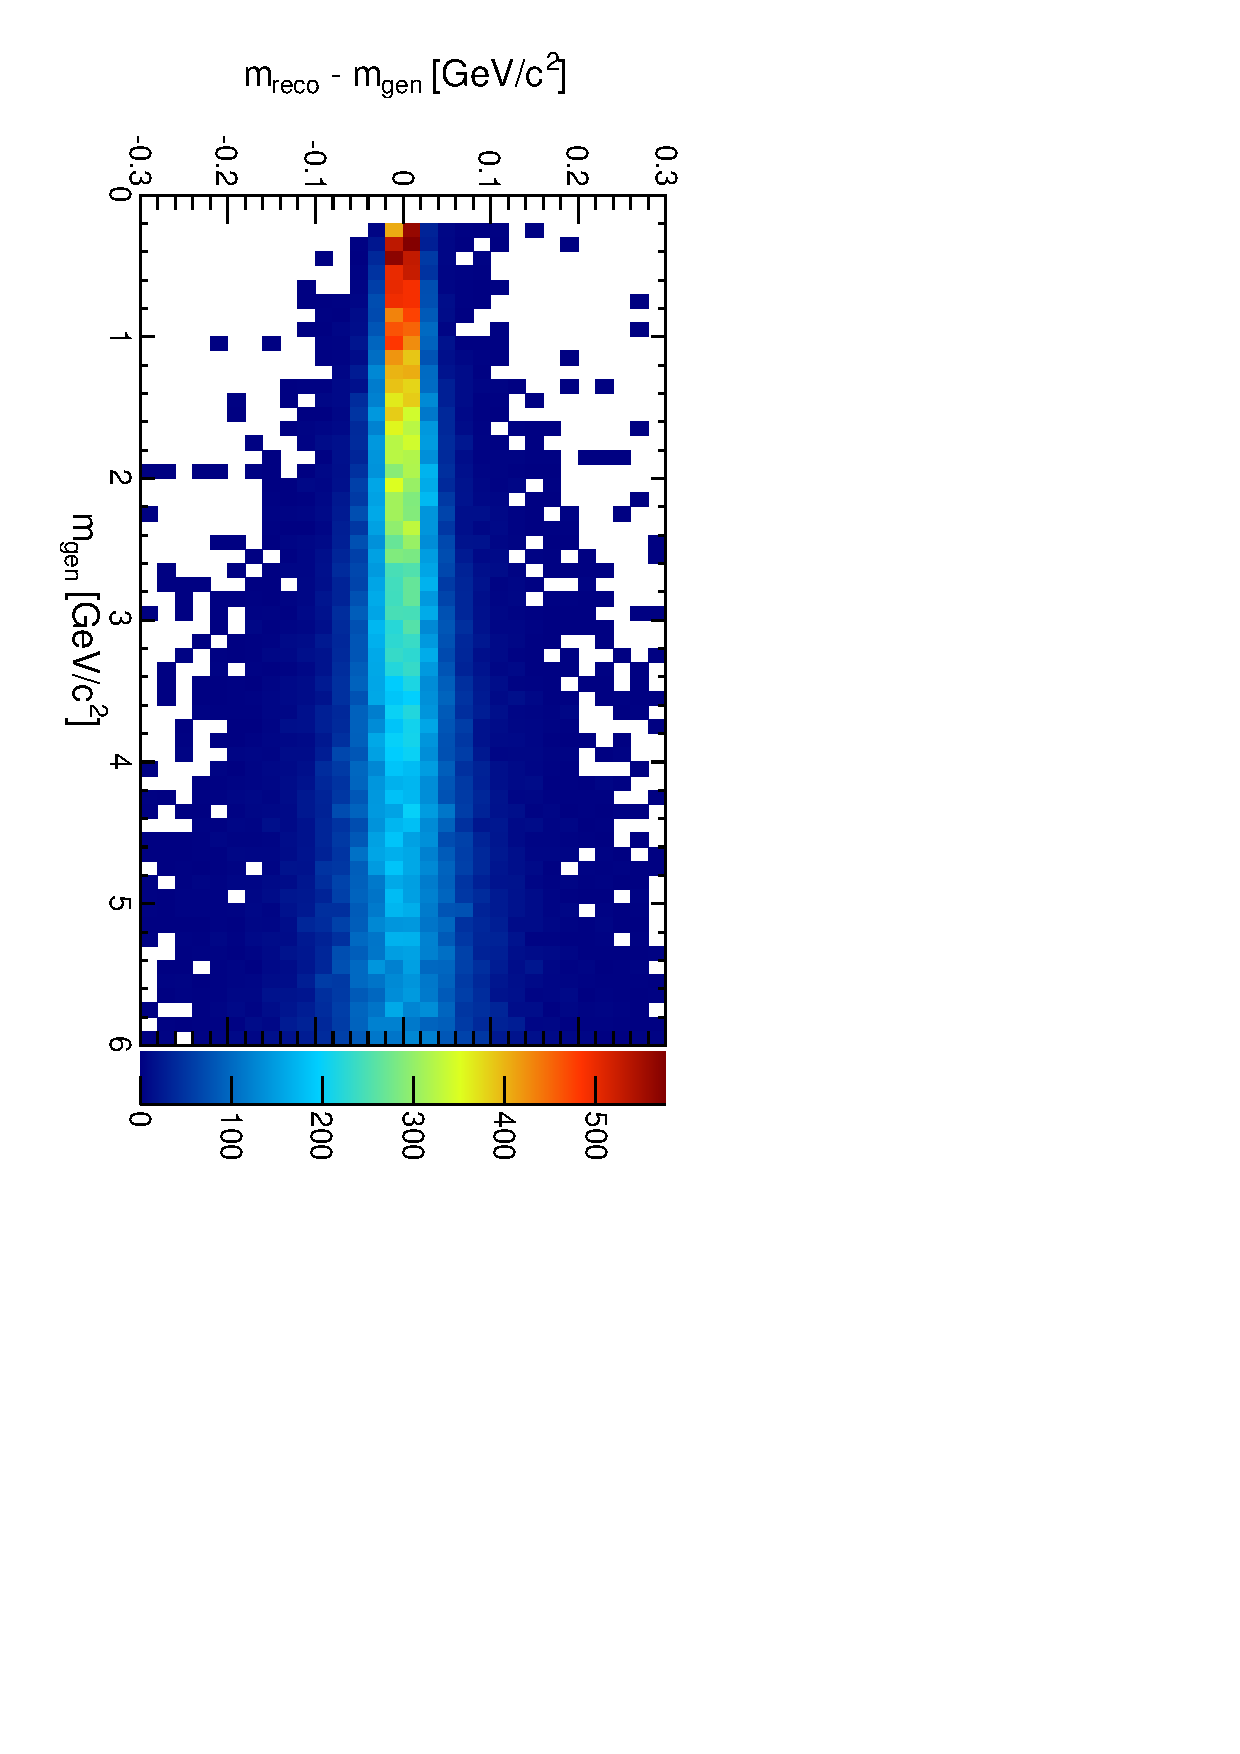
\includegraphics[height=\linewidth, angle=90]{deltamass_vs_mass.pdf}
\end{columns}
\end{frame}

\begin{frame}
\frametitle{Too many muons}

How often, in dimuon signal, do $\mu$-jets pick up an extra muon? \\
(Can worsen mass resolution and cause too many mergers)

\vfill
\begin{columns}
\column{0.8\linewidth}
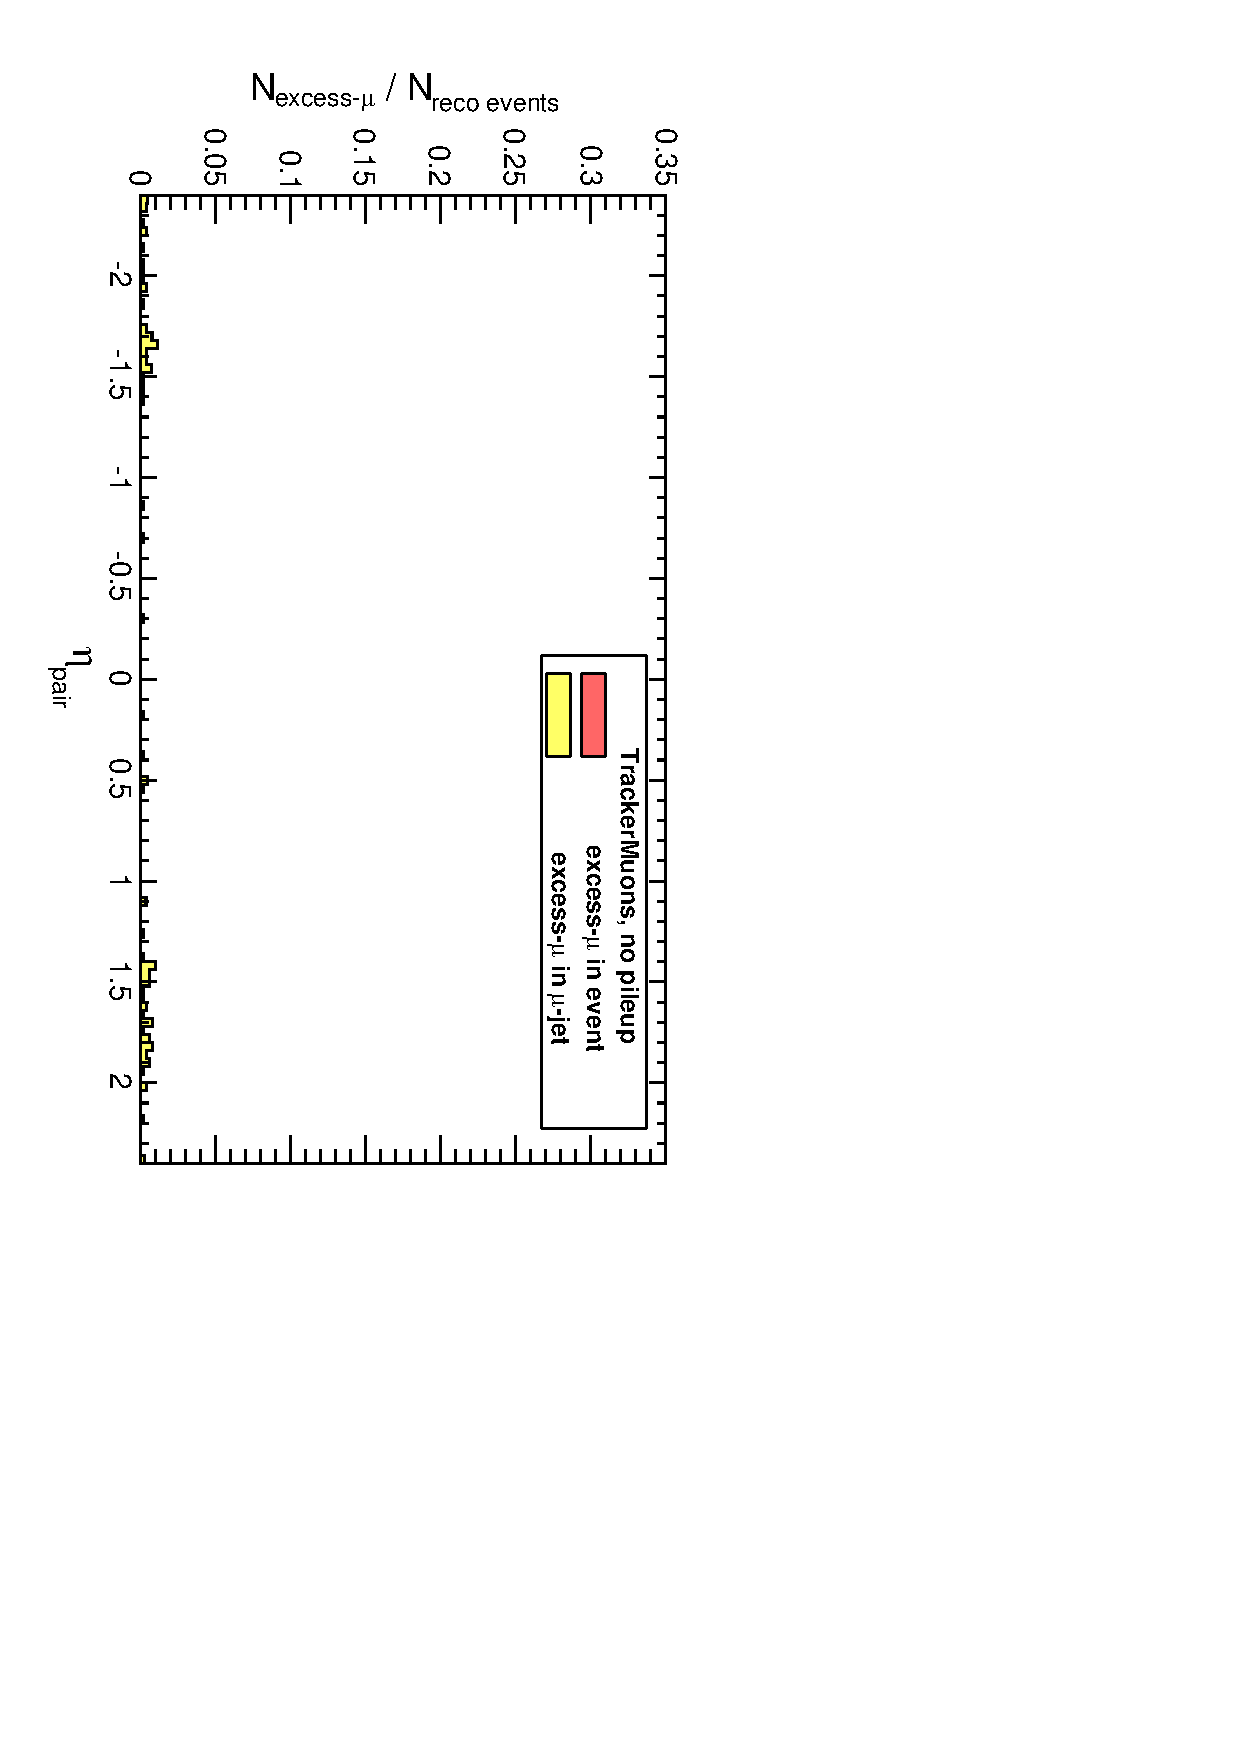
\includegraphics[height=0.5\linewidth, angle=90]{toomanymuons_TrackerMuonsGroupByMassAndVertexProbOrDeltaR.pdf}
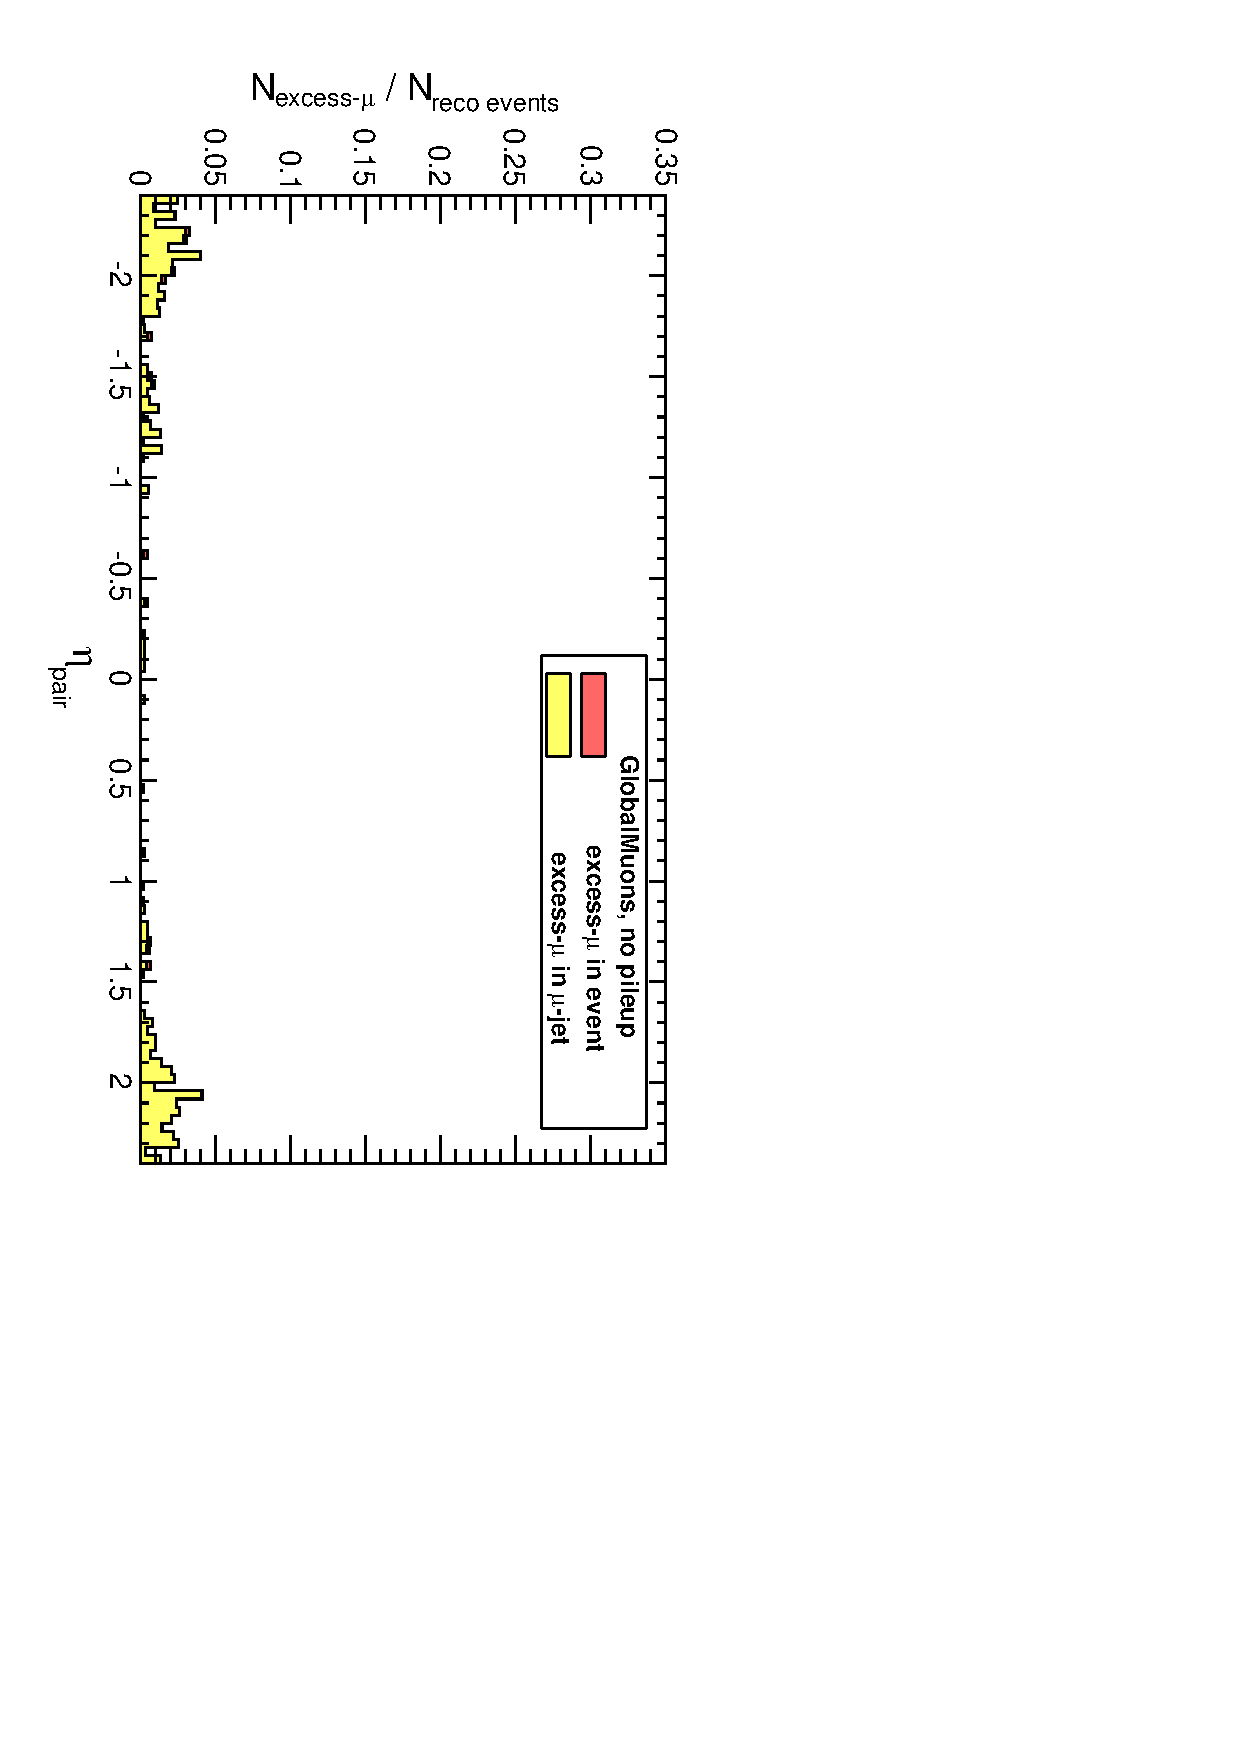
\includegraphics[height=0.5\linewidth, angle=90]{toomanymuons_GlobalMuonsGroupByMassAndVertexProbOrDeltaR.pdf}

\includegraphics[height=0.5\linewidth, angle=90]{toomanymuons_TrackerMuonsGroupByMassAndVertexProbOrDeltaR_pileup.pdf}
\includegraphics[height=0.5\linewidth, angle=90]{toomanymuons_GlobalMuonsGroupByMassAndVertexProbOrDeltaR_pileup.pdf}

\includegraphics[height=0.5\linewidth, angle=90]{toomanymuons_TrackerMuonsGroupByMassAndVertexProbOrDeltaR_pileup5.pdf}
\includegraphics[height=0.5\linewidth, angle=90]{toomanymuons_GlobalMuonsGroupByMassAndVertexProbOrDeltaR_pileup5.pdf}

\column{0.2\linewidth}
Depends on pile-up, naturally

\vspace{0.25 cm}
There are more TrackerMuons in high-pileup events, but not many of them get attached to $\mu$-jets
\end{columns}
\end{frame}

\begin{frame}
\frametitle{Too many muons}
The vertex compatibility criterion is very important!

\vfill
\begin{columns}
\column{0.6\linewidth}
\includegraphics[height=\linewidth, angle=90]{toomanymuons_TrackerMuonsGroupByMassAndVertexProbOrDeltaR_pileup5.pdf}
\column{0.4\linewidth}
Normal $\mu$-jet merging:

$(m_{\mbox{\scriptsize inv}} < 5\mbox{ GeV/}c \mbox{\bf\mbox{ and }} P_{\mbox{\scriptsize vertex}} > 1\%) \mbox{\bf\mbox{ or }} \Delta R < 0.2$
\end{columns}

\begin{columns}
\column{0.6\linewidth}
\includegraphics[height=\linewidth, angle=90]{toomanymuons_TrackerMuonsGroupByDeltaROrMass_pileup5.pdf}
\column{0.4\linewidth}
Normal $\mu$-jet merging:

$(m_{\mbox{\scriptsize inv}} < 5\mbox{ GeV/}c) \mbox{\bf\mbox{ or }} \Delta R < 0.2$
\end{columns}
\end{frame}

\begin{frame}
\frametitle{Displaced vertices}

\begin{itemize}
\item This is one of the discovery channels: a single dimuon with a highly displaced vertex (background is mostly near zero)
\begin{itemize}
\item HLT\_Mu5 puts a limit on efficiency because it requires a StandAloneMuon with beamline constraint
\item To go farther, we'd need to use a cosmics trigger or something (not worth it)
\item $\gamma \to e^+e^-$ 7-iteration tracking helps negligibly in the muon case (possibly because of GSF tracking)
\item GlobalMuons are about as efficient as TrackerMuons
\end{itemize}
\end{itemize}

\includegraphics[height=0.7\linewidth, angle=90]{dispvert.pdf}
\end{frame}

\begin{frame}
\frametitle{Displaced vertices}

\begin{itemize}
\item Particularly inefficient in the barrel-endcap overlap region
\end{itemize}

\vfill
\includegraphics[height=0.5\linewidth, angle=90]{pt2vseta1_0_10.pdf}
\includegraphics[height=0.5\linewidth, angle=90]{pt2vseta1_10_20.pdf}

\includegraphics[height=0.5\linewidth, angle=90]{pt2vseta1_20_30.pdf}
\includegraphics[height=0.5\linewidth, angle=90]{dispvert_vs_dispz.pdf}
\end{frame}

%% \begin{frame}
%% \frametitle{Outline}
%% \begin{itemize}\setlength{\itemsep}{0.75 cm}
%% \item 
%% \end{itemize}
%% %% \hspace{-0.83 cm} \textcolor{darkblue}{\Large Outline2}
%% \end{frame}

%% \section*{First section}
%% \begin{frame}
%% \begin{center}
%% \Huge \textcolor{blue}{First section}
%% \end{center}
%% \end{frame}

\begin{frame}
\frametitle{That's all for now}

Next: backgrounds

\vfill
Later: understanding a few of these unexplained issues\ldots

\label{numpages}
\end{frame}

\end{document}
